
%% this is a general purpose outline for preparing your thesis.  do not rigidly
%% follow this; feel free to discuss alternate structures with me.  your work
%% may have unique features that should be treated accordingly.  this template
%% that sets up the latex formatting and that contains my comments on the main
%% structures/paragraphs that you should develop for a masters or phd thesis.
%% the cover page is setup for a masters thesis; it is easily adjusted for a phd
%% dissertation.

%% as you can probably guess, in latex the ``%'' sign starts a comment, for some
%% reason i got in the habit of using two for main comments like this and have
%% done so ever since.  the comment goes to the end of the line.

%% to build this you will have to install the standard latex packages (if you
%% want to use the machine in my office that works.  the basic build command
%% sequence is (assuming the main latex file is titled ``thesis.tex''):

%% pdflatex thesis
%% bibtex thesis
%% pdflatex thesis
%% pdflatex

%% you do not actually need to do all four every time, but whenever you change
%% the citations/references file, you will have to go through the complete
%% sequence to have all labels resolve (basically latex is a one-pass system
%% that uses files to record references for use in later passes.

%% the way i've set this up, you will create your main prose in this file
%% (thesis.tex), your references will go in the bibtex file (refs.bib, i have
%% set yours up with my version for the parallel simulation literature) and your
%% figures should be stored as pdf in the figs subdirectory.  there are online
%% tutorials and books available to help you (i would stick to the online
%% stuff).  i can also help you resolve some things.  i will give you a quick
%% tutorial on the use of latex below (by example).

%% ------------------------------------------------------------------------

%% SOME COMMENTS ON THESIS WRITING

%% as you write your thesis, remember that this is a formal document; it is a
%% story and it should be interesting, but it should *not* be informal.  the
%% prose should be in 3rd person (no ``I'' or ``we'').  each paragraph should
%% stay in the same tense (prefereably present tense), and USE ACTIVE VOICE.

%% also, you will have to repeat yourself much more than you are confortable
%% with.  your writing has to carry the reader, you literally have to lead them
%% through your chapters.  you *will* end up restating things that you think are
%% obvious.  each chapter will have to begin with an intro to remind the reader
%% where you are going to take them (they will forget).  it is not obvious to
%% them, you have to explain.

%% remember, however, that it is a story, it is a technical story, but
%% none-the-less, you are developing an idea and you want potential readers to
%% pay attention to your prose.  make it a story that flows.  

%% each paragraph should focus on one topic and you may need to have transitions
%% between the paragraphs to help the reader make the transition through your
%% discussion.  generally you don't really have to do much to support
%% transistions.  develop your paragraph structure to present a coherent thought
%% from the topic sentence to the final sentence (of the paragraph).  most of
%% the time this will naturally lead you to the subsequent paragraph.  so in the
%% end, it *is* a story that is easy to read.

%% no contractions, ever!!  write formally, no ``something gets'' instead write
%% ``something obtains'', think about your wording.  use exactly the word you
%% want at each place in the prose; think about the subtle different definitions
%% similar words, ``between'' and ``among'' have drastically different meanings;
%% so do ``complex'' and ``complicated''.  be sure you understand the
%% differences.  you will live with a dictionary (online or on paper) as you
%% write this thesis, you will be surprised at how much you really don't know
%% about a word's real definition (you'd be surprised to know how much i still
%% use a dictionary).  finally, think about your words, expand your writing
%% vocabulary.  it can be really rewarding to write very good prose (and your
%% mechanics of writing are already solid).  what makes good writing superior is
%% the vocabulary and consistency.

%% be consistent!!  this is biggly important.  when you name something use the
%% same naming throughout; don't call something a subsystem in one chapter and a
%% subassembly in another.  select a name for your thing (e.g., signing device,
%% simulation object, etc) and stick with it throughout.  there is nothing more
%% confusing and offputting than to have the writer use multiple phrases to
%% refer to the same thing.  consistency is critical.  i could go on and on, but
%% let's stop here for now.

%% some more general comments:

%% 1. citations should have a preceeding space space use ``citation \cite{foo}''
%%    instead of ``citation\cite{foo}''.

%% 2. if you have a figure/table in the document, it must be discussed in the
%%    prose and you cannot simply say ``see \ref{pseudocode}'';  you must use
%%    the object name, such as ``see Figure \ref{pseudocode}'' (also capitalize
%%    the object name.

\documentclass[11pt]{book}

\usepackage{fullpage}
\usepackage{graphicx}
\usepackage{cite}
\usepackage{times}
\usepackage{url}
\usepackage{setspace}
\usepackage{fancyhdr}
\usepackage{ifthen}
\usepackage{listings}
\usepackage[section]{placeins}
\usepackage{xtab}
\usepackage{url}
\usepackage{amsfonts}
\usepackage{amssymb}
%%\usepackage{float}
%%\usepackage{wrapfig}
\usepackage{graphicx}
\usepackage[small]{caption}
\usepackage{subcaption}
\usepackage[ruled,vlined]{algorithm2e}
\usepackage{microtype}
\usepackage{color, colortbl}
\usepackage{pspicture}
\usepackage[pdf]{pstricks} 
\usepackage{rotating}
\usepackage{tikz}
\usepackage[nottoc,numbib]{tocbibind} 
%\usepackage[table]{xcolor}

\usepackage{url}
\usepackage{multirow}

%\usepackage{algorithm}
%\usepackage{algorithmic}
\DeclareGraphicsExtensions{.pdf,.eps,.svg,.pgm,.png}
\setcounter{topnumber}{2}
\setcounter{bottomnumber}{3}
\setcounter{totalnumber}{4}  
\renewcommand{\topfraction}{0.5}
\renewcommand{\bottomfraction}{0.95}
\renewcommand{\textfraction}{0.1}
\renewcommand{\floatpagefraction}{0.7}

\setlength{\abovecaptionskip}{3pt}
\setlength{\belowcaptionskip}{3pt}

\pagestyle{fancy}
\setboolean{@twoside}{false} 
\setlength{\headsep}{25pt}
\setlength{\headheight}{14pt}

    % EXTREMELY COMMON LaTeX PACKAGES TO INCLUDE:
    \usepackage{amsmath,amsthm, amsfonts,amssymb} % For AMS Beautification
    \usepackage{setspace} % For Single & Double Spacing Commands
    \usepackage[linktocpage,bookmarksopen,bookmarksnumbered,% For PDF navigation
                pdftitle={University of Cincinnati PhD. Thesis},%   and URL hyperlinks
                pdfauthor={Department of Electrical Engineering and Computer Science},%
                pdfsubject={UC },%
                pdfkeywords={UC}]{hyperref}
    \usepackage{lipsum}
    \numberwithin{equation}{section}
    \numberwithin{figure}{section}
\newtheorem{Theorem}{Theorem}[section]
\newtheorem{Definition}[Theorem]{Definition}
\newtheorem{Rule}[Theorem]{Rule}

\begin{document}



\thispagestyle{empty}

\doublespacing

\vspace*{0.5in}

\begin{center}
\LARGE{\textbf{Approximate Clustering Algorithms for High
Dimensional Streaming and Distributed Data}}


\vspace*{0.4in}

  {\large A dissertation submitted to the\\[0.20in]
    Division of Research and Advanced Studies\\
    of the University of Cincinnati\\[0.20in]
    in partial fulfillment of the\\
    requirements for the degree of\\[0.20in]
    {\bf DOCTOR OF SCIENCE}\\[0.20in]
    in the School of Electric and Computing Systems\\
    of the College of Engineering and Applied Sciences\\[0.20in]
    \date{\today} 
    by\\[0.20in]
    {\bf Lee A Carraher}\\
    BSCE, University of Cincinnati, 2008\\
    MSCS, University of Cincinnati, 2012\\}
  \vspace{0.5in}
  {\large Thesis Advisor and Committee Chair:  Dr. Philip Wilsey}
\end{center}

%\clearpage

%\newpage
%\thispagestyle{empty}
%\mbox{}

%\setcounter{page}{1}
%\pagenumbering{roman}
%\clearpage


\newpage
\thispagestyle{empty}
\mbox{}

\chapter*{Abstract} 
Clustering data has gained popularity in recent years due to an expanding opportunity to discover knowledge and collect
insights from multiple widely available and diverse data sources.  Data clustering offers an intuitive solution to a
wide variety of unsupervised classification problems.  Clustering solutions to problems arise often in areas in which no
ground truth is known, or when the arrival frequency of a data source exceeds the labeling capabilities of a human
expert.  Due to the continuous, fast moving nature of many common data streams, such as those from IoT (Internet of
Things) devices, social network interactions, e-commerce click-streams, scientific monitoring devices, and network
traffic, noise robust and distributed clustering algorithms are necessary.

Often, current clustering methods suffer from one or more drawbacks when applied to these demanding problems.  For
this reason, we propose a new method for data clustering that is noise resilient, and distributed with a predictable
overall complexity.  The principal claim of this research is that while many clustering algorithms rigorously optimize
a loss function, their convergence often results in finding a local minima that is indistinguishable from a less 
computationally rigorous optimization on an approximation of the data.  We propose that by removing the rigorous optimization 
requirement, we can achieve better scalability, and parallelism with comparable performance.  In this work we design a 
clustering algorithm along these lines that uses dimensional reduction and hashing to reduce the problem size while still 
attaining comparable clustering performance to other clustering algorithms. Our proposed method is more robust to 
noise with a lower runtime requirement, and greater opportunity for shared and distributed memory parallelism.

This work presents a set of methods for clustering high dimensional data for a variety of data source and processing
environments. The proposed \textsf{RPHash} algorithms share a commonality in that they all utilize locality sensitive hash (LSH)
functions and random projection (RP) to identify density modes in data sources.  They differ however in the operation space
and cluster region identification method. The algorithms presented are the \textsf{RPHash} algorithm, the 
\textsf{streamingRPHash} algorithm, and the Tree Walk RPHash (\textsf{TWRP}) algorithm.

We analyze the results of our developed algorithms on both streaming and at-rest data input environments.
Experiments on real and synthetic data demonstrate the advantages of our proposed clustering methods for 
streaming and at-rest data against common clustering algorithms.  Furthermore our theoretical analysis shows
that our runtime and memory complexities are effectively linear and sub-linear respectively, in terms of input.
Our principal claim that approximate clustering results are not substantially different than exact 
clustering methods with guarantee convergence to a local minima, is confirmed by these results. In addition
we demonstrate the potential gains in processing speed and parallelism.


\chapter*{Acknowledgments} 

%% put your acknowledgements here.
\begin{center}
 For My Friends, Family and Mentors
\end{center}

I would like to acknowledge the following people for their hard work and research effort on this work. People and organization
who without which none of this would have been possible.  First and foremost, my extreme gratitude goes out to my advisor: 
Prof.\@ Philip Wilsey.  Prof.\@ Wilsey's guidance not only in academic pursuits, but in so many aspects of my life, 
are truly appreciated.  His adherence to relentless delivery in terms of research development, publication and testing, are a
testament to his own commitment to scholarship.  Throughout our time working together, I feel that we have truly forged a bond of
friendship and colleague that far exceeds my expectation.  With my deepest gratitude I would like to say thank you Professor Wilsey.
I would also like to thank my fellow student researchers and co-authors: Sayantan Dey, Anindya Moitra. My co-developers
and fellow student researchers: Nick Malott, Tyler Parcell, and the Go-Lang \textsf{RPHash} group.  Finally I would
like to thank my friends and family, my parents, brothers and sisters, and my wife Alex. Alex your support and
encouragement has been an inspiration to me. Your courage and commitment in your own academic pursuits are things that I constantly
try to emulate and apply to my own research. I'd also like to thank the University of Cincinnati, Department of Engineering
and Applied Sciences, and the National Science Foundation for financial, equipment and facilities support.

%% these three lines will cause latex to automatically generate these entries
%% for you....nice.  you can comment them out if, for example, your thesis does
%% not contain any tables.
\tableofcontents \markright{ }
\listoffigures \markright{ }
\listoftables \markright{ }

\clearpage
\pagenumbering{arabic} \setcounter{page}{1}

 
\chapter{Introduction}

Humans and animals are often taxed with the task of categorizing things to augment their understandings beyond past
experience alone.  In essence humans and animals are generating models.  Model generation is a primary cognitive skill
that underlies our ability for prediction and understanding.  A primitive examples of this would be to decide whether an
animals is dangerous or not, based on past observations of the same species or similar looking animals.  A solution to
this decision problem would require a clustering of observations along with the outcome of dangerous or not.  A
clustering establishes a model for a given set of observations based on a metric of closeness in some parameter space.
In our example deciding whether an unseen animals is dangerous or not would likely include an evaluation of teeth shape,
relative size, eye location relative to head, etc.  In effect, forming two clusters of attributes relating to the
predator/prey nature of a given animal.

Human capabilities for implicit observation, and subsequent model generation far exceed anything possible with today's
computing systems.  The problem however arises from the limitations of human observations in both size and dimension.
While humans are good at building models for the tangible things around them, they are often unable to build similar
models for complex systems that reside in less intuitive spaces.  Mathematics and computing give us a probe into this
unattainable world through the use of numeric and graph based parameter embedding.  However high dimensional, numerical
spaces are still not very natural concepts for humans; while computing machinery on the other hand is quite at home in
with these concepts, in fact it's often a prerequisite for their use.

The development of mathematics and computing allow humans to augment abilities of prediction to develop models for
massive, unintuitive and fast changing systems.  These models allow humans to predict droughts, genetic predisposition
to disease, financial fraud, expose the underlying principles of particle physics, and many other useful areas that
improve our understanding, the quality of our lives, and protect the state of our planet.

Following the problem with correspondence between machines and concepts, the implicit parameter space is often encoded
into a more explicit objective space, such as a high dimensional euclidean space.  In this setting data can be
rigorously scrutinized for correlation and correspondence between observations.  Such correlation can then be distilled
into a model from which decisions can be made.

\section{Clustering}

Clustering has long been the standard method used for the analysis of labeled and unlabeled data and is a principle
occupation of statistical classification.  The effect of clustering data allows for identifying dissimilar and similar
observation in a dataset --- often unattainable by standard single pass statistical methods.  Single pass, data
intensive, statistical methods are often the primary workhorses for database processing of business logic and scientific
domains, while clustering is often overlooked due to issues of scalability \cite{clusters} and perceived complexity.  A
multitude of surveys \cite{clusters} have been made available comparing different aspects of clustering algorithms in
regard to accuracy, complexity, and application domain.  Due to this importance in machine learning, data clustering has
generated extensive interest in the computing and mathematics fields
\cite{anderberg1973,Samet,clusters,latent1,Hofmann,clusterstats,Zass2005}.  

Despite rigorous exploration, advancements in computing and countless variations, the Lloyd-type iteration $k$-means 
algorithm \cite{Hartigan, macqueen-67} remains the base for some of the most successful parametric clustering 
algorithms\cite{arthur-07}.  Of those the most successful clustering algorithm is the $k$-means algorithm. The $k$-means
algorithm seeks an optimal partitioning of a dataset into $k$ subsets that minimizes the within or inter-cluster distance.
The Lloyd-type/Lloyd-step $k$-means algorithm is an iterative algorithm for solving the $k$-means problem, that alternates 
between a cluster assignment step and centroid update step. These types of algorithms are important to consider because 
they not only embody many clustering procedures, but they also exemplify an intrinsic barrier to parallelism, namely the 
cluster update step, that is difficult to remove.

The success of $k$-means and similar clustering methods have facilitated enormous advances in nearly all scientific fields
as well as many social, business, and financial occupations.  Advances in clustering, in either scalability or speed
have a direct impact on the quality and timeliness of clustering results.  However, the unavoidable architectural
migration from single core processors with ever increasing clock rates, to static clock rates and increasing numbers of
cores, has introduced unique challenges for algorithm developers and data scientists.  Unfortunately, Lloyd-type
$k$-means is a data centric algorithm, with numerous sequential bottlenecks that do not lend themselves to parallel
implementation.

\section{Big Data Analysis}
Data analysis has a long been able to discovery latent data structures that were otherwise inaccessible by human
observation alone\cite{calderbank}.  
Recent advances in data aggregation along with the continuous roll-out of progressively more
advanced communication infrastructures has provided an unbounded sources of information.  This torrent of data, spurred
by industries insatiable appetite for deeper insights and user personalization, has pushed data analysis tasks well into
the realm of high performance computing.  While the processing of large-scale datasets is not new (VLDB is 42 years old this
year), the emergence of platforms for managing and frameworks for processing in the distributed setting has created a
new commercial market for large scale computing.  The trend is often referred to as \emph{Big Data}.  The development of
distributed frameworks is a natural progression of the parallel processing required in facilitating the transition from
single to multi core CPUs.  Furthermore the cost of large scale computing has decreased considerably thanks to cloud
services making it available to a larger community of researchers.

Where the general framework of distributed computing consists of a single data archive and attached processing nodes,
more recent frameworks attempt to take advantage of in place computing at the site of the data itself, taking advantage
of data locality and avoiding costly communication overhead. The common models for big data analysis consist of the 
MapReduce \cite{dean-08} and MPI \cite{mpi-spec-93} frameworks.  Both models take decidedly different approaches to parallelism.  
While MPI, or message passing interface, assists developers in the communication aspects of parallelism, the particular 
programming structure is mainly up to the developer.  Although not strictly enforced, the common MPI interface consists of
a master process that distributes data to worker processors, who then compute a partial solution that is then returned to the
master process for aggregation or further processing. MapReduce in contrast forces a more strict processing paradigm based on 
the functional programming structure.  MapReduce tries to avoid costly data communication overhead, by enforcing data locality
through functional programming structure.  This structure inverts the standard data distribution mechanism, by distributing 
the function to the data, instead of distributing the data to functions. These frameworks also often take care of other common 
but difficult to optimize, system level tasks, such as fault tolerance, low level communication and shared data storage 
architectures.  Both of these processing structure are amenable to our proposed algorithms.
 
\section{Security}
Another emerging requirement for data clustering especially in the distributed setting is security.  Patient privacy is
a high priority \cite{presidential}, and de-anonymization attacks have made it more difficult to provide anonymization
assurances beyond what is provided by data scrubbing alone.  Further, the decentralized geographic distribution of
medical care facilities prevents many tangential security measures often found in more centralized network topologies
(user$\rightarrow$organization).

\section{RPHash}
For these reasons we developed an algorithm to solve a parametric $k$-means clustering problem on distributed and
streaming datasets. In addition to the goal of distributed clustering, due to the ever increase possibility of data
breach, or method also provides reasonable security for data in transit and at rest.  We show that our solution offers 
comparable clustering performance to off-line solutions on a variety of synthetic and real world datasets.  Our 
solution uses bounded memory and achieves asymptotic linear scalability for a chosen set of configuration parameters.

Our algorithm, called \emph{Random Projection Hash} (\textsf{RPHash}), was expressly created to provide algorithmic
scalability on distributed datasets.  Many clustering algorithms have been converted to function efficiently on
distributed data, however they often have potential issues regarding asymptotic scalability \cite{Proclus},
dimensionality in which they are effective \cite{Clarans}, and robustness to noise.  Although many algorithms have been
proposed for parallel clustering, many issues are still present when applied to very large, high dimensional,
distributed datasets \cite{Clarans,Proclus,mpicluster,distributeddata,parclus}.  \textsf{RPHash} combines approximate and
randomized methods in a new way to solve these issues of scalability and data security under the assumption that
approximate clustering is qualitatively similar to exact clustering methods, due to noise, redundancy, data loss, and
the curse of dimensionality \cite{Beyer1999}.

In addition, we propose a variant of \textsf{RPHash} called \textsf{StreamingRPHash} that is similarly effective for the
streaming data setting.  Data streams in todays high tech environment can arrive continuously at a very fast rate.  They
are considered to be potentially unbounded and the user is primarily interested in recent data that keep track of the
emerging trends \cite{silva-13,braverman, shindler,aggarwal}.  Data streams are an increasingly common data model
owing to the pervasiveness of always on-line computing, and continuously updated measurements.  The stream clustering
data model puts two additional restrictions on the standard big data clustering model. First the complexity of the 
on-line step, in which vectors are added, must be sub-linear in $n$, the input size. The other requirement is that the
data can only be seen once, with some exception for temporary storage in a sub-linear in $n$ data sketch.

\section{Thesis Structure}
The structure of this the consists of presentation of required background information and related work, followed by 
our problem motivation, followed by a description of our proposed solution. We then test our proposed solution, and
discuss its strengths and weaknesses compared to other algorithms. More specifically, the remainder of this dissertation 
is detailed in the following paragraphs. 

In order to establish a common understanding of the clustering problem, various tools, notation and approaches, we give
a brief survey of related work, and background information.  Chapter \ref{bkgrnd} provides some background information
on material necessary for covering various preliminaries important to the description of our \textsf{RPHash} algorithm. 
The background section is organized into subsections corresponding to the problem decomposition of the \textsf{RPHash} algorithm,
in which each procedure corresponds to a section.
Chapter \ref{related} reviews some of the recent work with similar methods providing more scalable data clustering. 
We begin by discussing scalable solutions to low dimensional clustering, followed by scalable solutions to high dimensional
clustering.

To construct our reasoning and motivation for \textsf{RPHash} we present the next two chapters on motivations and algorithm description.
We follow the chapter with an added description of a related clustering method that attempts to use the data to define
the algorithm structures.
Chapter \ref{motive} introduces the initial goal of \textsf{RPHash}, and our early attempts at creating a scalable clustering
algorithm.  This section describes a drawback of the LSH based $k$NN problem that was realized to be useful for the
$k$-means clustering problem.
Chapter \ref{secrphash} provides a detailed description of the \textsf{RPHash} algorithm.  We describe the various components,
and the configurations of those components. Next we describe an extension of \textsf{RPHash}, \textsf{streamingRPHash} designed for 
the streaming environment. The following chapter
Chapter \ref{secadaptivelsh} first introduces a problem with LSH for data that is tightly clustered, but not uniformly 
distributed throughout the data space.  We use this understanding to design a new LSH algorithm that uses the input data 
to adaptively modify the specificity of the hash function.  We then propose a tree based clustering method that uses this type
of function to define the clusters as well. We then extend this solution to describe a general compressed space data structure
with applications beyond clustering.  

We conclude the dissertation with our experimental chapter, followed by a short chapter on the theoretical results, 
concluded by a set of conclusions, based on the findings from the previous two sections.
Chapter \ref{experiments} provides both clustering performance and timing results for \textsf{RPHash} and its
variants. The chapter begins with a description of the method that we compare \textsf{RPHash} against, the datasets
used for the comparison, and the metrics on which comparisons are made. Then an optimal baseline is established
through an exhaustive test of all possible configurations, to determine which is the best overall configuration.
The section continues by describing tests for each of the three proposed clustering methods, with plots and results
comparing them to other common clustering methods.  We also include a brief test of vector anonymity,
that demonstrates the security of our \textsf{RPHash} algorithms, as well as a test of the parallel speedup potential for
our \textsf{RPHash} algorithms. Chapter \ref{theory} provides theoretical asymptotic analysis for the proposed \text{RPHash} 
algorithms. We also include analysis for error propagation and techniques for decreasing the memory footprint of 
our tree based clustering method.  Finally, Chapter \ref{conclusions} contains a detailed analysis of the results
found in Chapter \ref{experiments}, followed by concluding remarks about the nature of clustering and the \textsf{RPHash}
approach to clustering. We conclude by presenting some ideas for future directions to for our line of research. 

%$k$-means clustering has long been used in academic, industrial, commercial, government
%and military applications.  Clustering has also found success among new technologies
%involving embedded systems in the recent movement to the so called Internet of
%Things(\emph{IoT}).  \emph{IoT} devices offer increased flexibility for data acquisition
%platforms while also suffering from a multitude of power, communication bandwidth,
%security, and storage problems.  In order to overcome some of these hurdles, clustering
%offers a way of minimizing communication and storage requirements by maintaining only a
%pertinent digest of collected data.  Furthermore, this minimization can result in positive
%effects to power consumption, and in the case of our solution, offers mitigation to data
%breach related security problems \cite{carraher-15}.

%Our algorithm, called \emph{Streaming Random Projection Hash} (\textsf{streamingRPHash}),
%is expressly created to provide algorithmic scalability while operating on large, high
%dimensional data streams.  While many stream clustering algorithms and
%conventional clustering methods converted to function on streaming data have been investigated, 
%they often
%have issues regarding asymptotic scalability \cite{Proclus}, dimensionality limits
%\cite{Clarans}, and robustness to noise.  A recent set of stream clustering algorithms
%have been proposed to address (with varying degrees of success) many of these problems
%.  \textsf{streamingRPHash} combines random projection
%and locality sensitive hashing in a new way to solve issues of scalability and data
%security for real-world high dimension streaming data analysis.

%The remainder of this paper is organized as follows:  Section \ref{bkgrnd} provides
%some background information necessary for covering various preliminaries
%important to the description of the \textsf{streamingRPHash} algorithm.  Section
%\ref{related} reviews some of the recent work with similar methods for data stream
%clustering.  Section \ref{rphash} provides an overview of the \textsf{streamingRPHash}
%algorithm.  Section \ref{experiments} contains experimental results and a brief
%summary of findings.  Finally, Section \ref{conclude} concludes the paper.

%% in this chapter you are providing any background information that would be
%% needed by the reader to facilitate their comprehension of your thesis topic.
%% basically you need to provide knowledge that your intended audience may not
%% have.  in this case, your indended audience should be young researchers and
%% experienced researchers (yea it can be tough).  you should plan your writing
%% to target that the lowest academic level of your readership.  in particular
%% you writing should target graduate students approaching their second year of
%% graduate study.  also, you are not necessarily writing to all possible
%% graduate students; you can target the particular class of researchers that
%% would normally read something in this topic space.  remember you are
%% providing background to facilitate understanding; you do not need to explain
%% everything about each topic, just enough that they can develop a reasonably
%% clear understanding that will allow them to read and comprehend the research
%% project that your thesis encapsulates.

%% start with an introductory paragraph explaining what this chapter
%% contains.  answer the question: what background are you going to cover?

\chapter{Background}\label{bkgrnd}

The beginnings of computing machinery, up until the introduction of the von-Neumann architecture, were narrowly focused
on the ambition of mechanizing rote data processing and analysis work.  Although today we find ourselves in a
multifaceted computing landscape arguably not likely envisioned by computing's forefathers, data analysis still occupies
much of the computing research space.  Perhaps rightly so, as advances in data analysis have had a profound impact on
virtually every field of scientific, economic, and social interest.  While the computing performance has grown
exponentially over the years many principal problems remain unsolved.  One such problem is the statistical
classification problem, with the implied definition of identifying an observations classification as induced by other
observations.  Classes in the computing parlance are more commonly referred to as clusters, and likewise the
classification problem is often referred to as cluster analysis.  Principal among clustering problems is the $k$-means
clustering problem defined in MacQueen's 1967 paper ``Some methods for classification and analysis of multivariate
observations'' \cite{macqueen-67} boasting over 18,000 direct citations.

\section{$k$-Means Problem}

By restricting observations to a vector space, the clustering problem can be described as a partitioning problem in
which the goal is to optimize the demarcations bounds to group similar observations.  The $k$-means clustering problem
extends this definition to allow a user defined number of partitions, $k$ that are specified, to separate the
observations into $k$ distinct groups.  Extending this concept we get a simple heuristic for the performance of a
particular clustering.  Given a set of vectors $x\in X$ partition the data space into $k$ clusters $\{C_1, C_2, ...,
C_k\}$ of vectors such that the \emph{Within-Cluster Sum of Squares Error} (WCSSE) metric is minimized over all possible
partitioning.  More formally,
$$
{\underset{C}{\text{argmin}}} {\overset{k}{\underset{i=1}{\sum}}} {\underset{x\in C}{\sum}}
||x-\mu_i||^2, 
$$
where $\mu_i$ is the mean of the points in a partition or centroid of the cluster $C_i$. 

Figure \ref{kmex} displays an example of a standard $k$-means algorithm run on Gaussian data clusters with nine random
starting instances.  The above optimization is WCSSE statistic is given with each clustering attempt.  The example shows
the success of the WCSSE criterion in identifying the ground truths of a dataset while variability in correspondence
between estimated centroid partitions and ground data points demonstrates a key drawback of hard margin data clustering.
In \textsf{RPHash}, a focus on high clusters in high dimensional space, minimizes the risk of overlap, discussed more formally in
the section on occultation (Section \ref{occultationSection}).

\begin{figure}
    \centerline{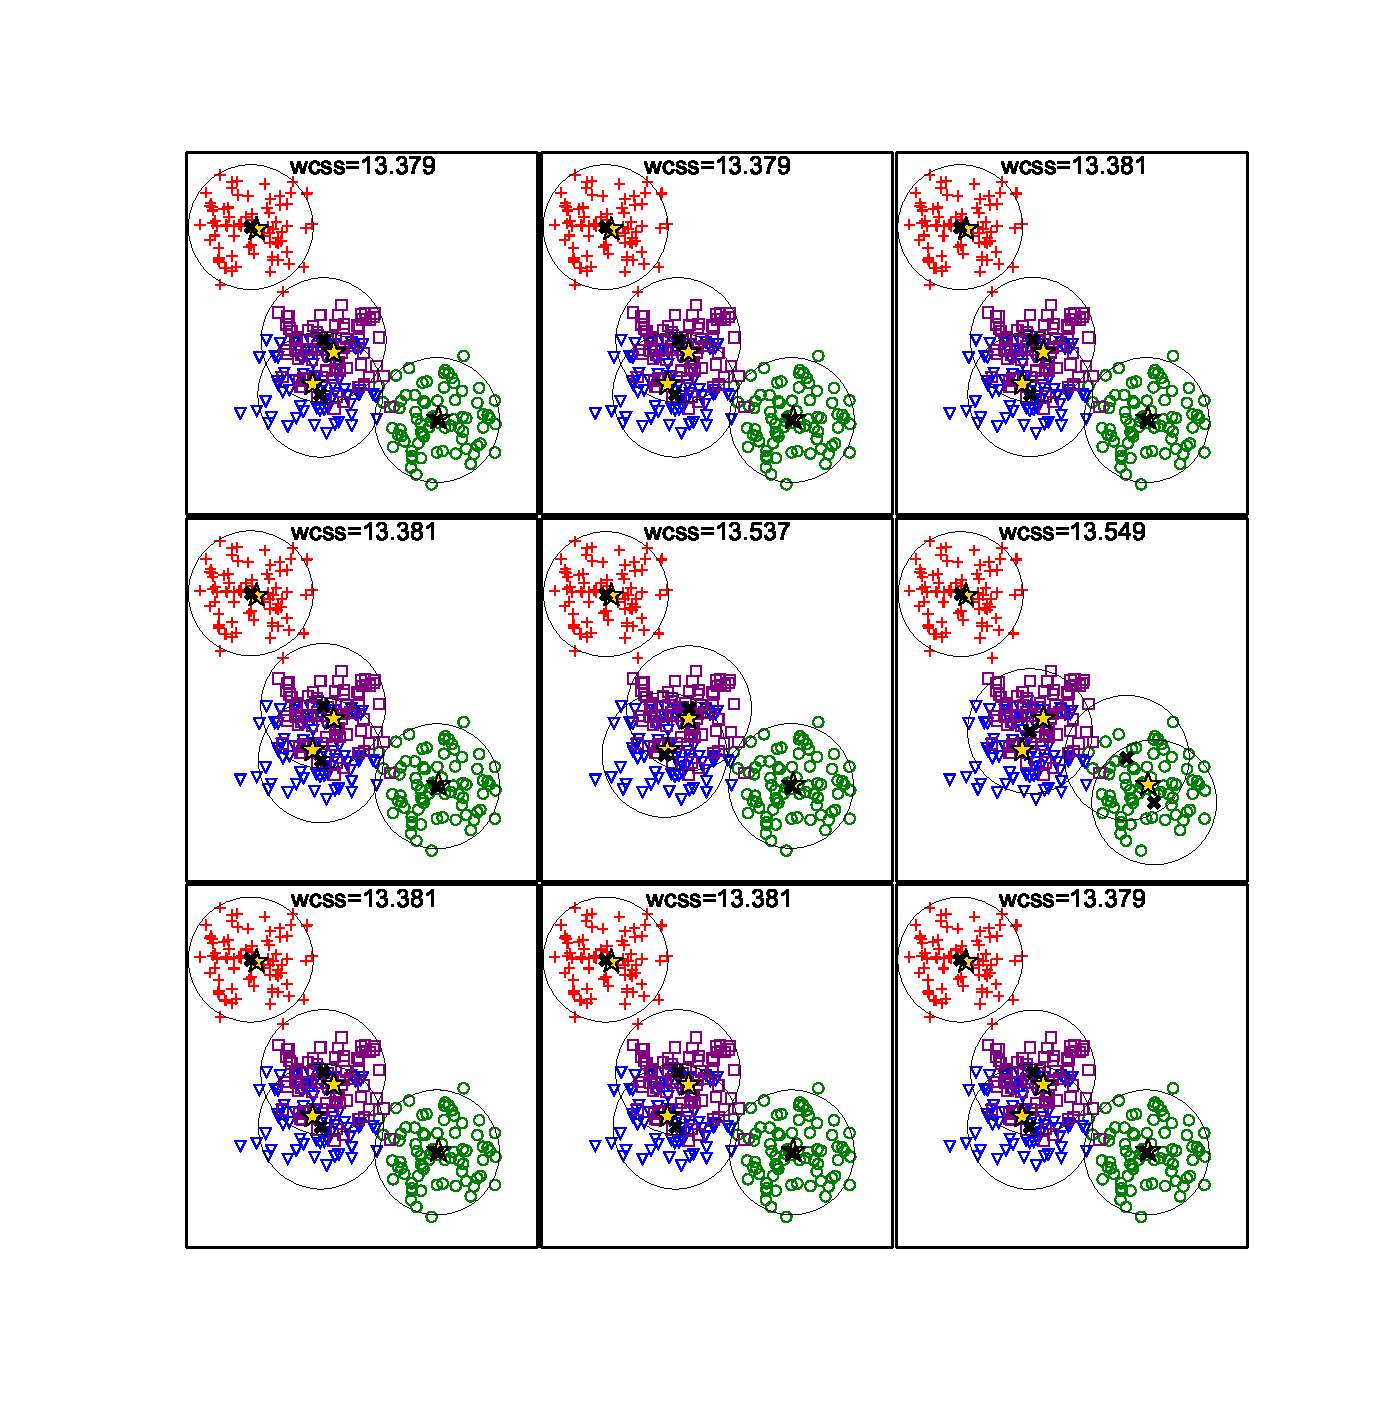
\includegraphics[width=1\textwidth]{figs/kmeanex}}
    \caption{Example $k$-means}{Example $k$-means on a dataset of 4 generated Gaussian clusters.  Gold stars mark the ground truth, and
      cluster symbol and coloring correspond to the vector's true membership.  Black X's mark the $k$-mean centroid
      estimates. The within-cluster sum of squares (WCSSE) is provided at the top of each plot.}\label{kmex}
\end{figure}

For points on a line, the $k$-means problem can be solved exactly in polynomial time using dynamic programming
techniques.  Unfortunately, this is a special case, and there is no known polynomial time algorithm for optimizing the
$k$-means criterion for generalized $\mathbb{R}^d$.  Following, if P$\neq$NP, optimizing the $k$-means heuristic is
Max-SNP/APX hard \cite{dasgupta08,Mahajan09}.  The two classes Max-SNP and APX are subsets of the NP class that deal
specifically with graph theoretic problems, and approximate optimization problems respectively.  These problems 
often have solutions that are can solve real world problems in polynomial(P) time, but are none-the-less in NP
for adversarially crafted problems.
Despite this somewhat dire outlook, APX problems such as $k$-means have
polynomial time bounded approximate solutions.  $k$-means not withstanding, $1+\epsilon$-approximate $k$-means can be
solved in linear time \cite{kumar}.  Furthermore, even simpler Lloyd-type algorithms tend to converge quickly on many
real-world datasets \cite{Jain}.

\section{Distributed Data}
Given the success of $k$-means algorithms and their relatively well behaved run time complexities, what need do we have
for another clustering algorithm?  While incremental algorithmic improvements result in shorter run-times they do not
often attack the fundamental issue of $k$-means's distributed scalability.  For this reason we propose an algorithm
that is specifically designed to overcome this issue that forestalls the communication requirement until the final
processing step.

\subsection{Distributed $k$-means}
A principal occupation of parallel computing research is speedup and the desire for a linear, or sub-quadratic
scaling.  Parallel speedup is the ratio of single compute node processing time versus parallel processing time or
$Speedup = T_s/T_p(n)$ , where $T_s$ is the time to process on a single node and $T_p(n)$ is the time to process in
parallel on $n$ compute nodes.  Of particular interest, is the shape of the ratio curve as $n\rightarrow \infty$, which
often is embedded in the underlying algorithmic structure.  The structure of the most common Lloyd-step $k$-means
clustering algorithm iteratively alternates between two steps, consisting of an assignment step followed by an update
step.  The assignment step, where centroids are assigned to their nearest representative cluster, can be made parallel by
processing data vector assignments in parallel.  However the update step, in which the cluster centroid is computed and
distributed to processors for the following assignment round, seems to be inherently sequential.  In distributed processing 
this issue is referred to as a sequential bottleneck or barrier synchronization.  Amdahl's Law gives the optimal speedup 
potential for parallel processing based on this ratio of required sequential $(s)$ code to parallel $(p)$ code.  More formally:
\begin{Theorem}[Amdahl's Law]
$$Speedup = {{1}\over{ (1-p)+{{p}\over{s}}}}.$$
\end{Theorem}

\begin{figure}
    \centerline{\includegraphics[width=.8\textwidth]{figs/speedup}}
    \caption{Amdahl's Law Speedup}{Amdahl's Law optimal Theoretical Speedup In a contention-less shared memory system for various
    parallel to total code implementations as a function of compute nodes}\label{aspeedups}
\end{figure}

In the case of Lloyd-step, $k$-means we can view the vector assignment step as parallel and the new centroid computation
as a sequential step.  Although this is perhaps an oversimplification, as centroid computation could also be
parallelized, Amdahl's Law speedup assumes contention-less accesses to shared memory, which does not exist in practice
as the number of processing nodes grows.  Instead additional communication overhead would be required, making the
centroid processing step sequential at best.  In Figure \ref{aspeedups} optimal speedups are shown for various ratios of
parallel to total code.

As discussed, even optimizing sequential to parallel code, will not overcome requirements due to network latency, 
memory contention and cache conflicts.  For these reasons,  recent work has focused on creating clustering
algorithms with lower communication overhead and fewer sequential bottlenecks. 

\subsection{Streaming Data}
In addition to being poorly suited for distributed analysis on static data, the standard $k$-means is not 
directly applicable to processing a continuous data stream. This is because, standard $k$-means requires a
pass through all of the data, to compute the final cluster centroids.  A requirement that is not available
in the streaming models. Next we define the streaming data model, its specific attributes and requirements.
In particular, the unbounded nature of the stream, implies that passing over all of the data, is not an option
for a streaming algorithm.
\begin{Definition}[Data Stream]
A data stream $S$ is a sequence of data vectors $v_1,v_2,...v_n \in V $ that arrive sequentially in time $t$ where
$t(v_1) < t(v_2) < ... < t(v_n) \forall v_i$, and the number of vectors $n$, is potentially 
unbounded ($n\rightarrow \infty$).  Each vector $v$ is of constant length, or is a variable length decomposable to 
constant length vector (e.g. words in sentences embedded in a sparse dictionary space).
\end{Definition}

Figure \ref{strmodel} provides an overview of the data stream model along with common attributes of many streaming
algorithms.  Data streams present a variety of challenges in both computational and storage complexity to clustering
algorithms.  The iterative nature of $k$-means requires that an entire dataset be accessible at any point in time.  Data
streams, however are potentially unbounded sequence of observations, with irregular arrival times.  Due to the unbounded
nature of streaming data, the entire set of vectors cannot realistically be stored in main memory.

\begin{figure}
    \centerline{\includegraphics[width=.8\textwidth]{figs/Streaming}}
    \caption{Streaming Model}\label{strmodel}
\end{figure}

In general there are three requirements that we regard as essential for streaming algorithms with $n$ observations, 
namely:
\begin{itemize}
 \item \textbf{Bounded Memory:} Due to the constraints of memory bandwidth in real machines, memory access patterns for
   data streams must be sequential allowing for one or a very small constant number of passes over the data.  The bound
   on the stored data, is sub-linear, and is usually regarded as either a predefined constant based on memory
   availability or $\theta(log(n))$.
 \item \textbf{Sub-Quadratic Processing Time:} Because the data stream is unbounded, it is infeasible to have an algorithm
   whose complexity is greater than $\theta(nlog(n))$ in regard to processing the entire data stream.  Or for each
   vector, no more than some constant$*log(n)$ steps may be performed.
 \item \textbf{Off-line-Step Complexity:} Due to the unbounded nature of the data stream, there is no reasonable start
   and end to the data stream.  As such, a streaming algorithm must be able to produce a result at any time throughout
   the evolution of the data stream, and in a reasonable amount of time.  While this amount of time is not strict, it
   invariably may only operate on the stored $\theta(log(n))$ data.
\end{itemize}

\noindent
In addition to the machine constraints presented by the streaming data model, streaming data often provides meaningful
temporal aspects.  One such attribute is changing trends over time.  Such trends as concept drift, occur often in the
semantic data space, and are a specific form of re-baselining in many other fields.  For this reason the concept of the
data stream, and subsequent clustering problems have been proposed \cite{silva-13} to capture these latent features.

\section{Sketching}

Following the requirements of streaming algorithms to have a bounded memory footprint, as with many big data problems in
computing accuracy is traded for memory.  One such method of lossy compression is the sketch data structure. The goal of
a sketch is to maintain an approximate record of the salient features of a dataset while not requiring that the entire
dataset be stored in main memory.  Sketch data structures have seen recent resurgence following the success of the
frequent directions algorithm \cite{libertyfreq}, hyperloglog \cite{hyperloglog}, counting \cite{cormode}, precision
sampling, and solutions to the $k$-Heavy-Hitters problem \cite{berinde}.

Sketching tends to offer one of two trade offs for memory, either lossy and sampling methods which older elements
ignored or forgotten or space saving, in which elements sketches lose accuracy over time.  \textsf{RPHash} resorts to the latter
exchange, and accept loss of accuracy over time.

\subsection{Count-Min Sketch}

One such data structure for space saving sketching is the Count-Min Sketch \cite{cormode}. The general idea is to
partition the element range into a finite set of discrete hash buckets, then update the bucket's value instead of
storing each element.  Due to the likelihood of hash collision in the element range, multiple copies with different hash
functions from the same family are updated in parallel.  To query an item's sketched value, all bucket sets are
searched, and the minimum of the searched buckets is returned.  The result of the minimum over multiple inaccurate
searches results in an amplification of accuracy for the searched element following, similar to minimum over chained
bloom filters.  Buckets update false positively often, but are never false negative for a given element, therefore the
minimum is the closest to the real count value.  Figure \ref{countmin} gives a diagram of this behavior for a toy
example.  Rigorous mathematical proof of the accuracy for this data structure has been studied in \cite{cormode3}.

For a positive only counter, the error in counting corresponds to the best of the $d$ approximate counts with error due
to noise from other counts, of $1/w$.  For $d$ hash functions if we chose $d = \log 1/\delta$ and $w=2/\varepsilon$ we
have an estimate for the count that is at most $\varepsilon N$ with probability greater than $1-\delta$.  Following a
proof in \cite{cormode2} using the Chernoff bound, the probability of returning a `bad' estimate is exponential in $d$.

\begin{figure}
    \centerline{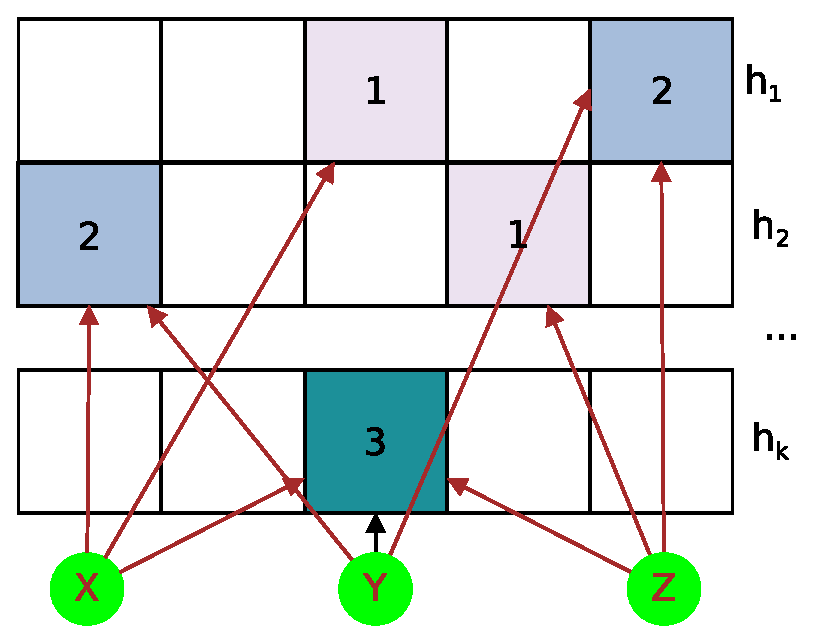
\includegraphics[width=.6\textwidth]{figs/countmin}}
    \caption{Count-Min Sketch}\label{countmin}
\end{figure}

\section{Dimensional Reduction}\label{rpprelim}

Dimensional Reduction is a key occupation for high dimensional data analysis.  Yet another face of the Curse of
Dimensionality, high dimensional data suffers from a loss of contrast between near and far points, making euclidean
metrics and even non-euclidean metrics useless as dimensionality grows.  This can be seen in the limit of the volume
occupied by a distance metric and an orthogonal space embedding approaching 0 as the embedding dimension grows.  Here we
give an informal proof of this approach.  The euclidean metric essentially carves out hyper-spheres in high dimensional
space as we can see from the distance function $d(x,y) = \sqrt{\Sigma(x_i-y_i)^2}$.  However, orthogonal embeddings with
many dimensions often distribute volume in coordinate space along rectangles.  We can see the ratio of the volumes of
these two geometric objects as dimensionality grows by taking the dimensional parameterization of the volume equation
for spheres and cubes with radius $r$ and side length $2r$.  Formally this derivation is

\begin{enumerate}\label{sphere2rect}
\item $ \text{Sphere\_Volume}(d) =  {{r^d\pi^{d/2}} \over {\Gamma(d/2+1)}}$
\item $\text{Cube\_Volume}(d) = 2r^d $
\item dropping constants, we get the asymptotic ratio:
$$
\mathlarger{\mathlarger{\theta}} \bigg({{\text{Cube\_Volume}} \over {\text{Sphere\_Volume}}}\bigg) =
{{(2r)^d \Gamma(d/2)} \over {\pi^{d/2}r^d}}
$$
\item replacing $\Gamma$  with Stirling's Approximation:
$$
= {   {  (2r)^d\sqrt{\pi d} ({{d}\over{2e}})^{d/2}   }\over {\pi^{d/2}r^d}  }
$$
\item dropping constants and simplifying:
$$
 = {{d^{d/2}(2/e)^{d/2}} \over {\pi^{d/2}}}
$$
\item taking the limit:
$$
\underset{d\rightarrow \infty} {\lim} { d^{d/2} \bigg({ {2}\over{e\pi}}\bigg)^{d/2}} = \infty.
$$
\end{enumerate}
\noindent
Even non-euclidean metrics exhibit this behavior.  This can be attributed to a more complicated analysis of the ratio of
the difference between the maximum distance and minimum distance divided by the maximum distance, often referred to as
contrast, approaching $0$ as $d\rightarrow \infty$.  A thorough investigation of this is given in \cite{zimek12,
  Aggarwal01, Beyer1999}

\subsection{Conventional Dimensional Reduction}
Conventional dimensional reduction techniques consist of the classic Principal Component Analysis (PCA) reduction which consists of
computing the directions of maximum variance in the data, and projecting the data along the a subset of vectors
corresponding to the greatest variance vectors.  PCA based reductions are useful and provide an embedding that optimizes
the error in the $L_2$-norm.  PCA reductions however require considerable computation, and are not suited for streaming
environments.  Frequent Directions \cite{libertyfreq} tend to mitigate these limitations but is are still fairly new in terms
of adoption.

Another technique for dimensional reduction is the t-SNE \cite{tsne} technique.  t-SNE is similar to PCA in its minimization
of an objective, however instead of minimizing the $L_2$-norm difference, it optimizes the Kullback-Leibler divergence.
Similarly it is not well suited for the streaming environment, as the minimization requires all data, and follows
a gradient descent approach to minimize the objective function.

\subsection{Random Projection}
Random projection is a method in which high-dimensional data vectors are projected down to a lower dimensional space by
applying a projection following some specifically crafted matrix.  One such example of an optimal distance preserving
projection would be the result of the truncated principal component projection.  Unfortunately PCA is computationally
complex and requires multiple scans over the entire input dataset.  However as the original embedding dimensionality
grows, the distortion between PCA projection and random projection tends to converge.  A random projection matrix is
composed of orthogonal vectors sampled from some random or quasi-random distribution.  Random projection can achieve a
bounded error distortion factor very close to the optimal $L_2$ norm subspace embedding that would otherwise result from
the principal component decomposition based projection \cite{bourgain1985lipschitz}.  The resurgence of the random
projection method of Johnson and Lindenstrauss was reinvigorated with the work of Achlioptas on Database Friendly
Projection that provided good subspace embeddings requiring minimal computation costs \cite{Achlioptas01}.

\subsection{JL Lemma}
The Johnson-Lindenstrauss Lemma defines the error bounds of random projection.  This formal bound for our projections
$f(\cdot)$ that preserves the distance between any two vectors $u$ and $u'$ with error $\epsilon$ is given as: 

\begin{Theorem}[Johnson-Lindenstrauss Lemma \cite{vempala}]
$$
 (1-\epsilon) \|u-u'\|^2 \leq \|f(u)-f(u')\|^2 \leq (1+\epsilon) \| u-u' \|^2
$$
\end{Theorem}

In Figure \ref{projex} results are given for a randomly generated dataset from $\mathbb{R}^{10000}$ of vectors that are
unit distance apart.  The vectors are randomly projected down to $\mathbb{R}^{10000}$, $\mathbb{R}^{1000}$,
$\mathbb{R}^{100}$, and $\mathbb{R}^{24}$ and the \textbf{L2} distance is calculated.  As the bound suggests, average
distance is consistently unit.  However, higher degrees of projection result in a greater occurrence of outliers and
overall increase in overall variance.

Under the optimal $\epsilon$-preserving mapping $f(\cdot)$, the Johnson-Lindenstrauss lemma results in a tight bound for
$u,u' \subseteq U$ and $n=|U|$, of $d \sim \Theta( {\frac{log(n)} {\varepsilon^2 log(1/\varepsilon) }})$.  The bound was
later applied to random orthogonal projections in Frankl and Maehara, and found to have a similar order on the bound for
the projected subspace dimensionality \cite{Frankl}.  Vempala gives a relaxation of the JL-bound for random orthogonal
projections, arriving at $d \sim \Omega(log(n))$ \cite{vempala}, with a scaling factor of ${\frac{1}{\sqrt{d}}}$ to
preserve approximate distances between projected vectors.
An additional benefit of using Random Projection for mean clustering is that randomly projected asymmetric clusters tend
to become more spherical in lower dimensional subspace representations \cite{bingham}.  Mean and medoid clustering
algorithms, such as \textsf{RPHash}, are predisposed to spherical clusters.

\begin{figure}
    \centerline{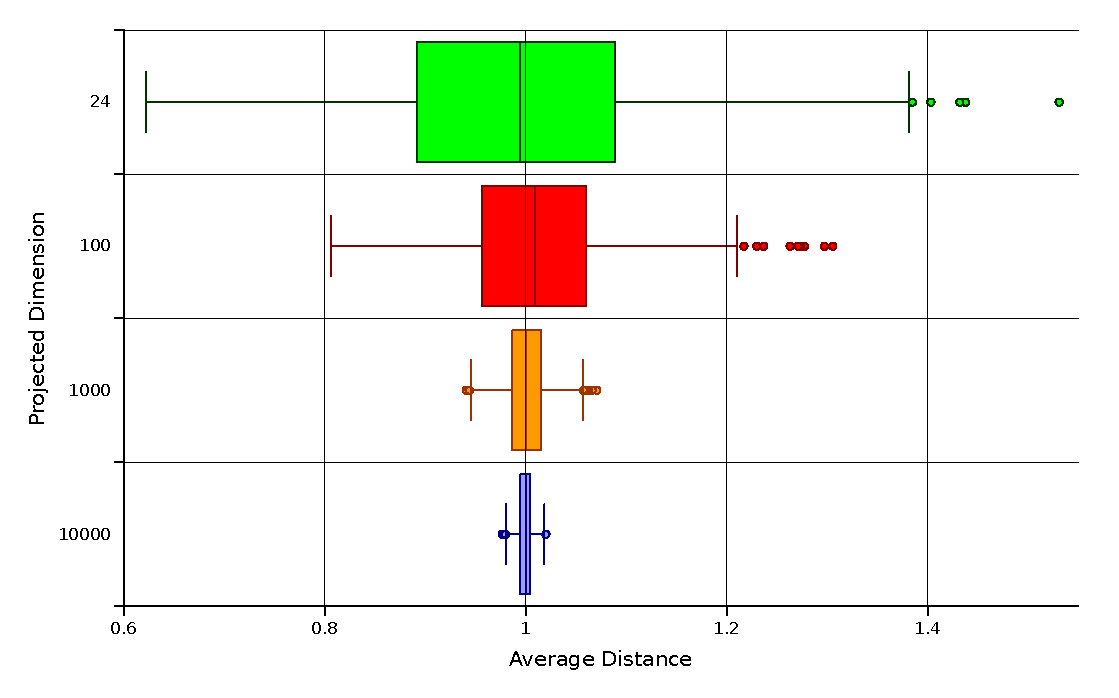
\includegraphics[width=.9\textwidth]{figs/projectiondimensionVSaveragedistance}}
    \caption[Experiment with Random Projection and Distance]{Example random projection dimension and expectation of distances for vectors that are unit distance
      apart.}\label{projex} 
\end{figure}

\subsection{DB-Friendly Projection}
Using the intuition that the dot product with a vector composed of zero mean Gaussian random variates, amounts to a
great deal of multiplication by values near zero, D. Achlioptas describe a far more efficient projection matrix with
surprisingly more favorable attributes than multiplication by a dense Gaussian matrix \cite{Achlioptas01}.  
These so-called DB-Friendly projections provide dimensional reduction that adheres to the JL-Bound, and in many cases
provide lower error embeddings than the more computationally intensive Gaussian matrix projection \cite{Achlioptas01}. 
Computed efficiently, the DB-Friendly Projection method requires $\theta(dm/3 )$ steps.
The DB friendly matrix is constructed as: $r_{ij}\in\textbf{R}$ is $m\times d$ as follows:
\[
    r_{ij}= \sqrt{1/d}
\begin{cases}
    +1, & \text{with probability } {\frac{1}{6}}\\
     0, & \text{with probability } {\frac{2}{3}}\\
    -1, & \text{with probability } {\frac{1}{6}}\\
\end{cases}\text{\cite{Achlioptas01}}
\]

\subsection{Fast Johnson Lindenstrauss Transforms (FJLT)}

Advances in compressed sensing and Restricted Isometry Property (RIP) have pushed the bounds of random projection to
nearly optimal and work efficient samplings of the input data following a realization that the underlying goal of random
projection is to evenly represent a mixture of the input space vectors.  To optimize this mixture, FJLT looks to the
Heisenberg principle in harmonic analysis, stating that the spectrum and signal cannot both be
concentrated \cite{ailon2006}.  The FJLT consists of a projection matrix product $\Phi = PHD$ that consists of two random
matrices, $P$ a sparse $m\times d$ Gaussian, $D$ a $m\times m$ diagonal ``coin-flip'' matrix, and $H$, the rank $m$
Hadamard matrix.  The resulting matrix projection requires only $\theta(m \log m)$ time where $m$ is the original
dimension.

\section{Space Quantization} 
Switching from the continuous spaces of random projections, we now consider the discrete space partitions induced by
lattices.  Optimal implementations of grid based clustering algorithms such as DBSCAN \cite{dbscan} and DStream \cite{cao-06}, require
that the data space be partitioned as evenly as possible.  Furthermore to avoid costly interprocess communication
overhead, a universally generative naming scheme must be established.  For known datasets, a perfect partition of the
data space can be produced by the Voronoi diagram \cite{Klein1988}.  In 2-dimensional space, Voronoi Diagrams can be
generated in $\Theta(n log(n))$-time \cite{Fortune}.  However, higher dimensional algorithms for Voronoi partitioning
have far less favorable runtime complexities \cite{Gavrilova2003}, making them inefficient for partitioning arbitrarily
high dimensions.
A solution to this partitioning problem is to sacrifice the optimal partitioning and accept a probabilistically  
close partitioning.  Such is the case with Locality Sensitive Hash (LSH) functions. 
LSH functions use collision probability dependent on distance to chain regular partitionings together to
approximate optimal partitions. Now we present a formal definition for LSH. 
\begin{Definition}[Locality Sensitive Hash Function \cite{datar-04}]
let $\mathbb{H}=\{h:S \rightarrow U\}$ is $(r_1,r_2,p_1,p_2)-$sensitive if for 
any $u,v\in S$
 \begin{enumerate}
   \item if $d(u,v) \leq r_1$ then $Pr_{\mathbb{H}}[h(u)=h(v)]\geq p_1$
   \item if $d(u,v) > r_2$ then $Pr_{\mathbb{H}}[h(u)=h(v)]\leq p_2$
 \end{enumerate}
\end{Definition}

Lattices, are an alternative, mathematical structure, that can partition infinite, fixed dimensional data spaces in a
generative way. We give an example of the $A_2$ Lattice in Figure \ref{lshex}.  Furthermore, lattices formed from binary codes (such as $E_8$ and Leech Lattice) have extremely
efficient nearest neighbor decoding algorithms.  A formal definition of a lattice constructed from a linear code is:
\begin{Definition}[Lattice in $\mathbb{R}^n$ \cite{Pless}]\label{latticedef}
let $v_1, ...  , v_n$ be $n$ linear independent vectors where $v_i=v_{i,1}, v_{i,2}, ...
,v_{i,n}$.  The lattice $\Lambda$ with basis $\{v_1, ...  , v_n\}$ is the set of all
integer combinations of $v_1, ...  , v_n$ the integer combinations of the basis vectors
are the points of the lattice.
$$\Lambda = \{z_1v_1+z_2v_2+ ...  +z_nv_n | z_i\in \mathbb{Z}, 1 \leq i \leq n\}$$ 
\end{Definition}

\begin{figure}
    \centerline{\includegraphics[width=.4\textwidth]{figs/2dLat}}
    \caption{$A_2$ Lattice Constellation}\label{lshex}
\end{figure}

\subsection{$E_8$ Lattice Decoder}

The $E_8$ Lattice or Gosset's Lattice provides an optimal sphere packing in 8 dimensions.  Furthermore, the nearest
neighbor decoding complexity of $E_8$ is relatively low, owing to its decomposition into $E_8 = D_8 \cup
<{1\over2}>+D_8$.  $D_8$ decoding entails a simple rounding technique among the vectors in $\mathbb{R}^8$ and an overall
parity check.  Further advancements \cite{SPLAG} in the decoding complexity of $E_8$ result in a decoder requiring only
72 steps.  However, due to $E_8$'s relatively low dimensionality, we must also apply a rudimentary outer decoding step
which simply splits a projected vector of dimension higher than 8 into multiple $E_8$ decodings.

\subsection{Leech Lattice Decoder}

The Leech Lattice is a unique 24 dimensional lattice with many exceptional properties \cite{Curtis,SPLAG}.  Of
particular interest to this work is the Leech Lattice's packing efficiency.  The Leech Lattice defines an optimal
regular sphere packing of 24 dimensional space \cite{leech} and serves nicely as a space quantizer for
\textsf{RPHash}.  Furthermore, the Leech Lattice, being the cornerstone of many intriguing mathematical
concepts, has various relationships with other sub-lattices that offer useful algorithmic decompositions.

Among some of the most efficient decoders for the Leech Lattice, Amrani and Be'ery's \cite{Amrani} decoder has a
worse-case decoding of only 331 floating point operations.  Although higher dimensional lattices with comparable packing
efficiency exist, the decoding complexity, in general, scales exponentially with dimension \cite{Tarokh1,Agrell}.

\subsection{Spherical Locality-Sensitive Hashing}

Another method of space partitioning applicable to data where the vector norm is 1, or rather lies on the surface of a
hypersphere, is the Spherical LSH technique of Terasawa \cite{SLSH}.  Spherical LSH uses an inscribed regular polytope
to partition the surface of the sphere where vertexes of the polytope correspond to partition regions.  Although other
regular d-polytopes such as the d-simplex and d-hypercube exist, we focus on the d-orthoplex, following the favorable
collision probability per distance, which results in Table 1 of \cite{SLSH}.  The $d$-orthoplex is a regular d-polytope
with $2d$ vertexes corresponding to the positive and negative axis per dimension of a $0$ centered unit hypersphere
embedding.  The nearest vertexes can be searched among the $2d$ vertexes following the max dot product method given in
\cite{SLSH}, resulting in a search time complexity of $\theta (d^2)$.  The $d$-orthoplex has the benefit over $E_8$ and
Leech Lattice decoders of allowing for arbitrary projection dimensions, with the disadvantage that it is only strictly
applicable to vectors lying on the surface of a hypersphere.

\subsection{Collision of LSH Functions}
As stated above, a desired trait of an LSH function is a discriminative collision probability curve with respect to
inter-point distance.  In Figure \ref{prcollision} we give the collision probability curve for set of LSH
functions: The Leech Lattice($\Lambda_{24}$), Multi-$E_8$, Spherical LSH (SLSH), and the Gaussian $p$-Stable distribution.  
Notable, multi-$E_8$ gives the tightest overall curve, with $\lambda_{24}$ following closely in terms of discrepancy ratio
for distance $p = {{r_1} \over {r_2}}$.

\begin{figure}
    \centerline{\includegraphics[width=.8\textwidth]{figs/prcollisions}}
    \caption{Probability of collision as a function of distance for various decoders for vectors in
      $\mathbb{R}^{24}$}\label{prcollision} 
\end{figure}

\section{Differential Privacy}

Security is another issue that arises in the distributed clustering problem.  Medical, financial, and proprietary
commercial data are often targets for clustering that have security requirements not addressed in the local clustering
setting.  Data privacy is often important in machine learning due to the sometimes sensitive nature of records in a
dataset.  Distributed and streaming data analysis applications have additional security requirements due to the
sometimes insecure transport mechanisms between processing nodes.  The cryptographic concept, differential privacy,
provides some solutions to these problems.  The result is often a trade-off between privacy and data loss or additional
processing requirements.  This general concept is referred to as Differential Privacy \cite{diffpriv}.

\subsection{$k$-anonymity}

$k$-anonymity is privacy technique that defines a number $k$ of records that are equivalent based on the record's
attributes.  Generalization and suppression are employed, such that data utility is not lost, and the $k$-anonymity
constraint is met for some $k$ \cite{Aggarwal2008}.  An intuitive example would consist of a set of patient records with
various attributes.  One such attribute could be age, employing the rounding technique, one could coerce two records to
being equivalent, by changing the exact age to a range of ages such as 18-25, instead of 19, and 23.  Such a obfuscated
dataset would have $k=2$ -anonymity.

\subsection{$l$-diversity}

An extension of $k$-anonymity, $l$-diversity attempts to protect the attributes as well as the records.  $l$-diversity
overcomes some of the flaws in $k$-anonymity, by requiring that a dataset has at least $l$ different values for each
attribute.  Common ways to achieve $l$-diversity are random sampling and additive noise.

\section{MapReduce}
MapReduce \cite{dean-08} and similar programming structures have become popular in recent years with the so called big data revolution.
These architectures abstracted out the often tedious and difficult management tasks of maintaining a fault tolerant,
distributed, processing system.  Furthermore, they made heterogeneous computing on commodity hardware the norm for big
data processing that it is today.  This change allowed more people and businesses to take advantage of large scale
processing while not requiring specialized hardware or in the case of Platform as a Service (PaaS) architectures removed
the need for hardware altogether.

MapReduce is a distributed processing framework in which the focus is data locality facilitated by a functional
programming approach.  Common to functional programing, the Map and Reduce functions perform specific operations on data
instead of the data-flow approach in which data is distributed to processors.  The map function is an operation that
maps data to a discrete set of keys, while the reduction function aggregate the keys.  From the distributed computing
context this process scales well so long as the key-set and reduced data are not exceedingly large compared to the
original data.  By strictly adhering to Map and Reduce functions, data can be distributed horizontally across a set of
systems during the data collection phase, and small data bandwidth operations can be broadcast (scatter) to be performed
on the processing node's local data.  The key reduction step is also optimized in this framework, as key aggregation can
be performed on a peer-to-peer basis (gather).  While these processing method are not new, perhaps the more long lasting
result is the proliferation of freely available distributed processing frameworks.

\begin{figure}
    \centerline{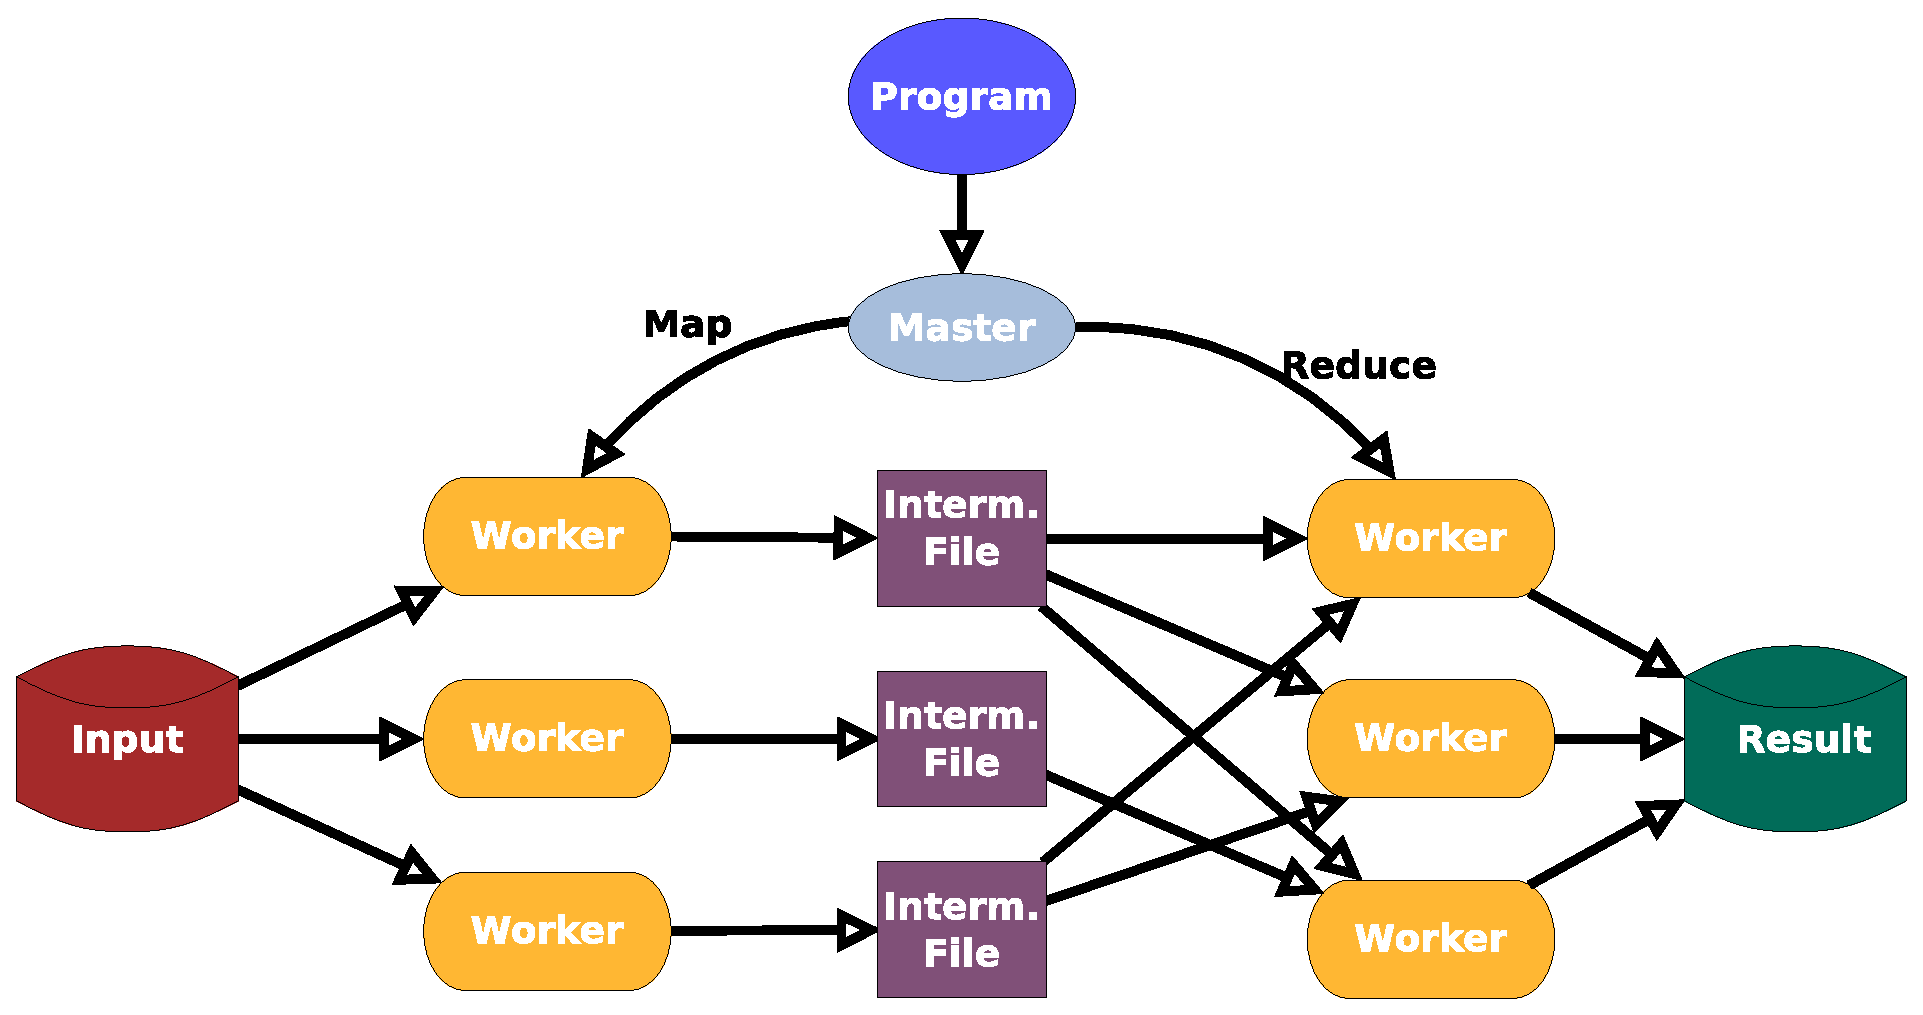
\includegraphics[width=.8\textwidth]{figs/mapreduce}}
    \caption{Map Reduce Step}\label{mr}
\end{figure}

Hadoop from the Apache Foundation is a popular version of the map-reduce framework written in Java.  Hadoop also includes a 
distributed file system (HDFS \cite{shvachko-10}) as well as monitoring tools, and extensions various computing tasks such as machine learning,
namely the Mahout package.

Spark \cite{chowdhury-10,zaharia-10} is an extension of map reduce that performs in memory data manipulation while also allowing for more flexibility
in the processing sequence.  In standard map-reduce, only a single shot, map (read from disk) and reduce (write to disk)
operations are preformed.  Various meta-frameworks have mapped the map-reduce task, however they strongly incurred the
disk IO processing bottleneck.  Spark continues the functional approach to distributed processing, namely map and
reduce, but extends it to utilize in memory storage and multiple applications of map and reduce.  In addition to
supporting a more generic map-reduce distribution, Spark also support streaming data processing.  Streaming data
processing consists of a continuous stream of data distributed to processing nodes, with periodic `off-line'
synchronization processes.  Figure \ref{strmodel} depicts a point in time in the streaming model with earlier and past
time represented by a darkening of the data stream squares.  In this work it is adequate to interpret each block as not
necessarily uniform sized, batch of data vectors evolving over time.  For each batch of vectors, a sub-linear sketch of
the data is updated.  Periodically or at the request of a user, the sketch can be analyzed by an `off-line' step that
yields a result given the current state of the data stream.  In the case of a clustering algorithm this would be a set
of centroids.  We refer the reader to Silva \cite{silva-13} and Aggarwal \cite{Aggarwal2007} for an extensive analysis
and definition of various goals and methods in data stream clustering.  In this work we will focus on finding fixed $k$
non-moving centroids.


\chapter{Related Work}\label{related}

Clustering is a historically well developed and long lived field in mathematics and computation.  The modern
computational incarnation of clustering likely started with Stuart Lloyd's work in 1957 at Bell Lab's \cite{lloyd-57}.  In the 60 years
since this development, volumes of work have been devoted to developing new methods for identifying clusters and testing
their performance.

Despite an exponential worse-case complexity of $k$-means (where $P\neq NP$) \cite{Vattani}, many real-world problems tend
to fair much better under Lloyd's type of solutions to $k$-means optimization than theoretically optimal solutions.  For
this reason, clustering massive datasets with $k$-means, although suffering from unbounded complexity guarantees, often
yields qualitatively good results close to the optimal $k$-means solution.  Due to the approximate solution's real-world
proclivity towards revealing useful results, randomized methods such as sampling and random dimensional reduction are
often utilized in overcoming complexity growth.  The use of these methods in clustering began with density and grid
based scanning algorithms.

Clustering algorithms have a variety of applicable taxonomies often differentiated by data type, cluster shape,
inference model, and so on.  In this work we will focus mainly on a particular type of clustering distributed algorithms
for clustering high dimensional Gaussian clusters. Below we list some similar clustering methods to RPHash, split by type
and process setting.\\
\noindent
\textbf{Distributed clustering algorithms:}
\begin{itemize}
 \item canopy clustering \cite{mccallum}
\end{itemize}

\noindent
\textbf{Classic algorithms:}
\begin{itemize}
 \item $k$-Means \cite{Hartigan}
 \item $k$-Means++ \cite{arthur-07}
\end{itemize}

\section{Density Based Clustering}

The first set of clustering algorithms began with density based scanning methods.  These methods tend to work well on
spatially separated datasets with relatively low dimension.  A common clustering problem for these types of algorithms
would be on geo-spatial data, in geographic data systems (GIS) and image segmentation.  The algorithms DBScan
\cite{dbscan}, Clique \cite{clique}, and CLARANS \cite{Clarans}, respectively, represent a successful progression of the
density scanning techniques.

%% LEE: streamingRPHash or just RPHash??

DBSCAN proceeds in a conceptually similar manner to \textsf{RPHash} in regard to partitioning the data space
and counting the number of data vectors within a partitioned region.  The first set of parallel clustering algorithms
began with density based scanning methods as the process of building out clusters can take advantage of memory locality
(\emph{e.g.,} spatially near vectors are also near in memory).  Although density scan algorithms are an example of
parallel designed algorithms such as \textsf{RPHash}, they often show weaknesses in accuracy when scaling the number of
dimensions.  A proposed solution mentioned below to this problem is Proclus \cite{Proclus}.

\section{Clustering in Projected Space}

Another important set of algorithms related to \textsf{RPHash} are projection based clustering algorithms.  The natural
commonality among these algorithms is that instead of clustering over the entire data space, they deal with a projected
subset of the data.  The immediate benefit is a reduced computational complexity.  Various other benefits of random
projection are discussed in Section \ref{rpprelim}.  Clustering by random projection, similar to \textsf{RPHash}, are
explored in \cite{fernrandom,alweighted06,avogadri09}, but they often strongly violate the limits of the
\emph{JL}-lemma, resulting in occultation.  The concept of random projection clustering is not new, having been explored
in a variety papers involving high dimensional data clustering.

Proclus \cite{Proclus} was an even early example of projection clustering that used random 1-dimensional projections to
reduce the dimensionality of a clustering problem.  The 1-dimensional projections were then ensembled to create a
consensus of clusters.  A proof of the convergence of projected $k$-means clustering is given in Boutsidis
\cite{Boutsidis}.  The merits of random projection are further discussed in \cite{Dasgupta2000} who suggest that random
projection not only compresses sparse datasets making them computationally more tractable but also may help overall
accuracy by alleviated round-off issues caused by non-homoscedastic variance by generating more spherical clusters in a
more dense subspace.

In addition to Proclus, various other methods and analysis have been proposed for clustering with random projections
that provide bounds on the convergence and limits of random projection clustering.  Florescu gives bounds on the scaling
and convergence of projected clustering \cite{florescu09}. Their results closely follow the logic of Urruty
\cite{Urruty2007}, and find that the number of orthogonal projections required, is logarithmic in $n$, the number of
vectors to be clustered.  Related to the arctangent of the angle between any two distinct clusters the probability of a
random projection plane offering a good partitioning increases exponentially as the number of dimensions in the
projected subspace increases.  Bingham \emph{et al} provide examples of projected clustering well below the JL bound
\cite{bingham} and Bartal \emph{et al} make these assertions mathematically rigorous showing that the projected subspace
is independent of the data's original dimensionality \cite{bartal}.
%FEATURE Selection
Proclus used an assumption similar to \textsf{RPHash} regarding high dimensional data's sparseness.  Feature subset
selection offers a way of compacting the problem as well as removing artifacts.  Many subset selection algorithms have
been explored \cite{subset1,subset2,Yang,Kaski98}.  They generally require difficult to parallelize iterative gradient
descent \cite{Amdahl} or tree traversal \cite{Freeman}.  Random projection is performed on the data to compress it to
spherical clusters \cite{Dasgupta2000} in a dense subspace.  An iterative method for k-medoid search, similar to CLARANS
\cite{Clarans} is then used to identify clusters.  Although the proposed method is successful in accelerating larger
dimensionality problems ($~d=20$) it does not have the overall proposed scalability of \textsf{RPHash}.  This is due to
Proclus being based on an ultimately iterative algorithm, containing inevitably sequential code, and therefore lacking
indefinite scalability \cite{Amdahl}.

Other clustering by random projection algorithms have been explored that are similar to \textsf{RPHash}, but for
projections on the line.  These so called cluster ensemble approaches \cite{fernrandom,alweighted06,avogadri09} use
histograms to identify cluster regions of high density much like \textsf{RPHash}.  Although, as suggested in Florescu and
Urruty, the single dimension approach may be plagued by issues of occultation, and exponential convergence as $d$
increases.  Figure \ref{3dto2d} shows a brief example of projection occultation for Gaussian clusters in $\mathbb{R}^3$
space, projected to $\mathbb{R}^2$ space.  In Figure \ref{3dto2d} it is clear that even modest reductions of $3$
dimensions to $2$ dimensions can yield unwanted results.

\begin{figure}
    \centerline{\includegraphics[width=.70\textwidth]{figs/3dto2dproj}}
    \caption{Random Projection of Gaussian Clusters in $\mathbb{R}^3\rightarrow \mathbb{R}^2$}
    \label{3dto2d}
\end{figure}
%%Recently, a streaming version of $k$-means, Streaming $k$-means \cite{stream$k$-means} was 
%%proposed that uses divide and conquer techniques along with sampling to solve the
%%Approximate $k$-means clustering problem.

\section{Streaming Algorithms}

Streaming Clustering is subset of clustering that consists of clustering data that arrives in a streaming fashion or as
batches overtime.  The goal is to perform a similar partitioning as the static case for other clustering methods with
the requirement that we cannot randomly access seen data, nor see future data.  CluStream \cite{clustream} is a
framework for clustering dynamic streaming data.  CluStream stores micro-clusters, consisting of a over sampling of the
$k$ desired clusters.  The $k$ desired partitions are emitted at chosen time intervals, through some off-line clustering
method, thus leading to on-line and off-line clustering phases.  In addition addition, CluStream allows for dynamic
clustering by introducing Pyramidal Time Frames that allow micro-clusters to split and merge over time.  The CluStream
framework is applicable to a variety of streaming clustering methods, and its on-line/off-line phase decomposition is
the general framework adopted by Tree-Walk \textsf{RPHash}.

A common baseline algorithm for streaming clustering, called streaming $k$-Means\cite{braverman,streamkmeans} derives much of its update process from
the original Lloyd-type $k$-Means iteration.  However, similar to CluStream, an over-estimate of micro-clusters is
maintained, to be further clustered in an off-line step.  Streaming $k$-Means' similarity to $k$-Means, is in its process of
assigning incoming vectors to their nearest representative cluster.  However due to the ground state of not having
clusters, the decision whether to aggregate with an existing cluster or form a new one must be made.  In general this
can be done with some sort of inter-cluster similarity or intra-cluster dissimilarity metric.  Some of the drawbacks to
streaming $k$-Means is that it is highly dependent on the input order of the data stream.

%% sliding window
In addition to random projection methods, recently streaming algorithms for data clustering are also considered
\cite{Har-Peled,braverman}.  The general setup of these algorithms consists of a diminishing objective bound that
tightens as the stream is processed.  The processor updates the core-sets of pseudo-centroids when data are within the
objective bound, and disregards data outside that bound.  Streaming $k$-means algorithms perform well on data streams,
but have the drawback of requiring that data be `well-clusterable'.  \textsf{streamingRPHash} uses a similar core-set
approach, but instead of choosing core-sets based on computed distances from current centroids, it maintains a data
structure of dense partitioned regions.

CSketch is a streaming algorithm for generating clusters over massive-domain datasets \cite{aggarwal}.  It shares much
in common with \textsf{streamingRPHash}.  In particular, CSketch applies the Count-Min Sketch data structure to update
candidate centroids by updating the centroid location and not just a count.  Incoming centroids must then search for
candidate clusters in order to find the nearest centroid.  In \textsf{streamingRPHash} we use the LSH decoding of
projected points to immediately find the nearest candidate cluster in the Count-Min Sketch data structure.  Furthermore,
our hashing algorithm is intrinsic to the decoding step, and does not require a supplementary hashing scheme.

\section{Tree Based Clustering}

A later enhancement to \textsf{RPHash} referred to as adaptive LSH (ALSH), and its subsequent alternative tree-walk,
off-line-step shares similarities with the decision tree clustering discussed in ``Clustering Through Decision Tree
Construction'' \cite{Liu2000}.  Liu \emph{et al} describe an implicit clustering approach that instead of grouping
observations by inter-cluster similarity (such as WCSSE), attempts to differentiate dense clusterable data from
uniformly distributed background data.  Like decision trees, the CLTree algorithm recursively splits the data set into
groups of similar observations.  An unsupervised optimization condition is required to overcome the discord between
unsupervised clustering, embedded in a supervised learning algorithm like decision trees.  The condition, mention
previously is to assume points belong to either a dense cluster or are part of some random uniform background noise.  To
differentiate clusters, from noise Liu \emph{et al} optimize the information gain criterion C4.5 at each split.  As such,
CLTree iterates over the dimensions in the data space, splitting the dataset with the hyperplane that maximizes the
information gain criterion for that dimension.  A further modification of the information gain criterion, by which the
algorithm ``looks forward'' a set number of levels of the tree, prevents decision plane from directly cutting clusters
in half.  The method is primarily concerned with lower dimensional clustering tasks for less than 20 dimensions, and has
roughly linear complexity over dimensionality and dataset sizes up to 20 dimensions and 500000 records respectively.
These results are on par with the results for \textsf{RPHash}.  A caveat with their results is that each cluster was
specifically generated to occupy a completely independent subspaces from the other clusters, and that subspace spans less than
five dimensions.


\chapter[Motivations and Precursors of RPHash]{Motivations and Precursors of RPHash}
\chaptermark{Pre-RPHash}
\label{motive}

In this chapter we will describe the motivations behind the \textsf{RPHash} algorithm, and give an overview of the \textsf{RPHash}
algorithm's goals.  The general idea of \textsf{RPHash} is motivated by a particularly degenerate case of the LSH-based $k$
nearest neighbors ($k$NN) problem known as $cr$-NN.  Briefly, the nearest neighbor problem is the problem of finding the
closest analog in a database to an unknown data vector.

\section{Bad $k$NN}
In one-dimension, the NN problem is solvable in log-time via a binary search of the dataset.  Similarly, in
two-dimensions it is also solvable in log-time via the point location algorithm over the Voronoi partitioned dataset.
The log bound unfortunately fails as dimensionality grows greater than 2, mainly due to the exponential growth of the
Voronoi region set $n^{\theta(d)}$.  Data structures such as k-d Trees\cite{Bentley-75} can be constructed to provide log-time average search
complexity for uniform datasets up to about 32 dimensions ($N >> 2^d$, $N=$ size of Database).  Beyond that however, k-d tree
search tends to degenerate into the linear scan search algorithm.  Naively this problem can be solved by the linear scan
algorithm (shown in Algorithm \ref{linearscan}) which consists of sorting a list of distances between the query vector
and all vectors in the dataset then returning the nearest $k$ vectors.

\begin{Definition}[Nearest Neighbor] \cite{Samet}\\
Given a set of vectors $P$ in $R^d$ and query vector $q$ return $k$ vectors $p\subseteq P$ such that
$p=\text{Argmin}\{dist(p',q)\}$, where dist is some metric function.
\end{Definition}

\begin{algorithm}
\RestyleAlgo{boxruled}
\caption{Linear Scan, Query $q$, dataset $X$\label{linearscan}}
\DontPrintSemicolon
$k$NN$ = X[0:k]$\\
\ForAll{$x \in X[k:n]$} 
{	
      \If{$\lVert x,q\lVert_2 < \lVert q,k$NN$[0]\lVert_2$}
      {
	$k$NN$[0]=x$\\
	$k$NN$ = sort(k$NN$)$\\
      }
}
\textbf{Return:} $k$NN
\end{algorithm}

This algorithm requires that we compute distances between every vector in the dataset and our query vector $\theta{nd}$.
If we could somehow omit vectors that we know are not anywhere near our input vector, we could certainly speed up our
calculation and possibly solve $k$NN in a sub-linear time.  This is the intuition of the LSH-$k$NN algorithm.
Previously discussed LSH functions can be used to winnow the field of candidate near neighbors that need to be searched
via the linear scan method. A considerable amount of computation can be avoided by performing this large volume
reduction on the query dataset provided some error is tolerable.  The basic outline of LSH-based $k$NN is given in
Algorithm \ref{lshnn} and Algorithm \ref{lshnnq}.

\begin{algorithm}
\RestyleAlgo{boxruled}
\caption{Preprocessing on Dataset X \label{lshnn}}
\DontPrintSemicolon
\ForAll{$x \in X$} 
{	id = LSH\_Hash(x)\\
	$T$[id].add$(x)$\\
}
\textbf{Return:} $T$
\end{algorithm}
\begin{algorithm}
\RestyleAlgo{boxruled}
\caption{Query $k$ nearest to $q$ in X, using hashtable $T$\label{lshnnq}}
\DontPrintSemicolon
id = LSH\_Hash($q$)\\
\textbf{Return:} linear\_scan($T$[id],$k$)\\
\end{algorithm}

Assuming the LSH\_Hash function is sufficiently discriminative, an appropriately chosen locality sensitive hash
functions can achieve a complexity bound of $\theta(n^\rho+log(n))$ where $\rho$ is determined by the selectivity of the
hash function.  LSH-$k$NN is a highly successful solution to the nearest neighbor problem in high dimensions.  However,
a degenerate case of the LSH-$k$NN structure occurs when the candidate field becomes quite large.  These degenerate
cases represent an outlier condition for $cr$-NN algorithm, and often contributes to the algorithm's worse-case
performance.  While this outlier example presents a problem to $cr$-NN, viewed under a different problem requirement, it
becomes beneficial for quickly identifying candidate density modes.

In Figure \ref{lshclust} we give give a toy example of the basic concept for or proposed Random Projection Hash algorithm.
The example contains 4 vectors, 3 of are somewhat close to one another in $\mathbb{R}^2$.  The space is randomly bisected along
4 partitioning plains, corresponding to 4 hash functions and 8 regions.  Inspecting the high cardinality hash buckets, we see
they often, but not always, correspond to high density regions.  In this case our small cluster of 3 items. The
correspondence between high cardinality hash buckets and high density partitions, forms the basis of our algorithms.
\begin{figure}
    \centerline{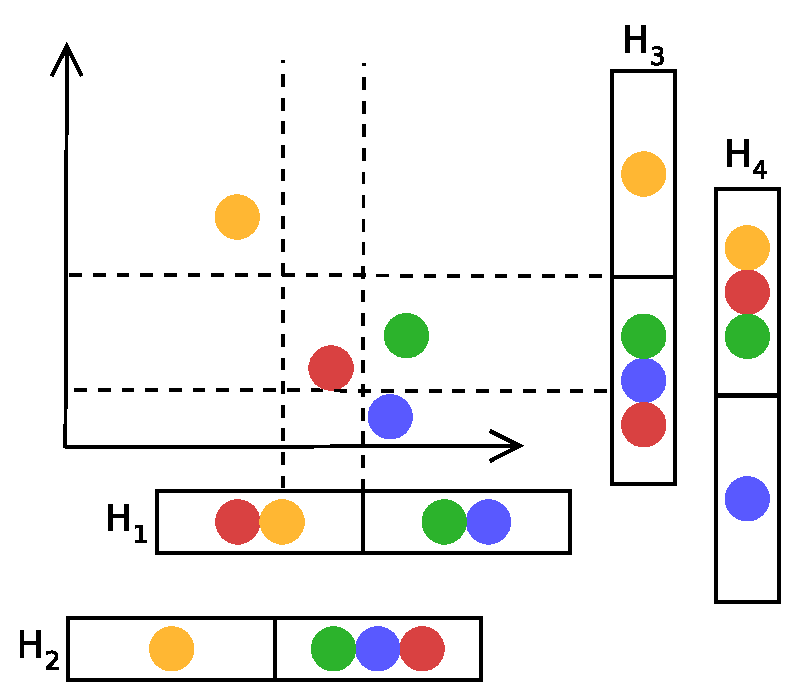
\includegraphics[width=.6\textwidth]{figs/multiLSHClustering}}
    \caption{Example of an orthogonal LSH on $\mathbb{R}^2$ Data}\label{lshclust}
\end{figure}

\section{Cardinality Shift Clustering}
Previous work on graphics processing unit (GPU) accelerated $cr$-NN \cite{carraher} lead to a generous speedup per GPU core for bulk NN search.
One problem that could take advantage of this acceleration to bulk NN search is the LSH accelerated Mean Shift algorithm
of Li \emph{et al} \cite{Li09}.  Although this still remains an interesting use case, a more interesting case was
investigated where the generative nature of decoder functions could be used to optimize interprocess communication in
distributed systems.  In this dissertation, vectors would be assigned to processing nodes using the LSH function, resulting
in better vector locality.  Furthermore this proposed method would use LSH bucket cardinality as a proxy for the
computational and communication inefficient mean shift step shown in Figure \ref{unreferencedFigure}.

\begin{figure}
\[
\overset{\rightarrow}{x}= {{\sum_{x_i\in N_(x)}
{K'({x-x_i})\overset{\rightarrow}{x}}}\over {\sum_{x_i\in N_(x)} {K'({x-x_i)}}
}}
\]
\caption{Mean-Shift Iteration \cite{Li09}}\label{unreferencedFigure}
\end{figure}

This algorithm is referred to as \emph{Cardinality Shift Clustering} (CSC).  The overall iteration of CSC is similar to
the mode finding step in the mean-shift clustering algorithm \cite{comaniciu-02, carreira, meanshift} with a
focus on scalability and low compute node interdependency.  To get better vector-node locality and minimize
communication overhead a two step course-grain and fine-grain shift is considered.

\subsection{Fine-Grain Iteration}

The fine-grain iteration is similar to mean-shift clustering update step except that it occurs on a finite set of
vectors contained within the bounds of a the partition of the well known Leech Lattice.  Due to this lattice's fixed
dimensionality, conversion between vectors of $\mathbb{R}^d$ and $\mathbb{R}^{24}$ must be performed by random
projection and the pseudo-inverse(or $\epsilon$-suitable inverse) of the projection \cite{bingham}.  Furthermore, this
clustering occurs on a per-compute node basis (Figure \ref{csc}, region \textbf{II}) and each compute node is assigned a
subset of lattice regions (Figure \ref{csc}, region \textbf{I}).  The lattice region IDs are generative and can be
assigned either by truncating the ID mod the number of available compute nodes or some other more advanced load
balancing technique.%% based on the number of vectors per compute node.

Using techniques from Andoni \cite{Andoni} and an addition from Carraher \cite{carraher2}, computation of the function
$N(\cdot)$ of near neighbors for a given point can be performed in nearly optimal $\Theta(n^\rho)$-time.  For a Leech
lattice hash function where $d \leq24$, $\rho \approx 0.2671 $ \cite{Andoni}, while linear search requires $\Theta(d
n)$-operations.  This gives an internal clustering complexity of $\Theta(k n^{1+\rho})$ where $k$ is the maximum
neighborhood size.  By adding the random projection aspects to this iteration, it is believed we will achieve some
tempering to the error surface across multiple projections which may help avoid some local minima of the density modes
by smoothing out point discontinuities.  Furthermore, the sigma value for an Gaussian, $N(\mu,\sigma)$ distribution in
the random projection may allow us to control tempering.

\subsection{Course Grain Iteration}

Due to the $\Theta(n^2)$ complexity of mean-shift clustering, we attempt to mitigate vector to vector communication
scalability by replacing it with a lattice-region to lattice-region course communication step.  All lattice-regions
contain a finite set of vectors.  In CSC we use the cardinality of the sets as weighted components for generating the
course-grain shift vectors, again using the standard kernel mean shift algorithm (Figure \ref{csc}, region
\textbf{III}).  The shift vectors are then broadcast to all computing nodes in the system.

\begin{figure}
    \centerline{\includegraphics[width=.8\textwidth]{figs/csc}}
\caption{Cardinality Shift Clustering}{\textbf{I.} Initial lattice assignment, \textbf{II.} Fine Grain Iteration,
  \textbf{III.} Course Grain Iteration, \textbf{IV.} Updated Positions}\label{csc}
\end{figure}

\subsection{Update Step}
Per compute node, the update step consists of updating all vectors current positions by applying the results of the
course-grain mean-shift vectors within a lattice region for a random projection (Figure \ref{csc}, region \textbf{IV}).
After this, we invert our random projection matrix and apply it to all the vectors giving us a set of (number of random
projections) vectors for each vector in our original $\mathbb{R}^d$ space.  We then average the vectors various random
projections to attain an $d$ dimensional representation that is near the actual result of a full mean-shift clustering
iteration for that vector.  Once the representations of the shifted vectors are averaged in $\mathbb{R}^d$, we again
project the vectors down to 24-dimensional space.  The assumption here is that the global shift will have altered the
lattice-regions for vectors near the borders of a region.  The vectors that have new lattice-region assignments first
check the current compute node for the new lattice-region assignment(a mod lattice ID can easily be tested here).  If
they are not contained in the current compute node, the vector must be sent to the compute node containing its new
lattice-region assignment.  The amount of transfer needed is hopefully minimal and point-to-point.

\subsection{Stopping Condition}

The number of lattice-region assignments should naturally decrease as vectors are pulled toward higher density
lattice-regions.  By counting the number of inter-compute node vector communications (the number of vectors whose
lattice-region assignments have changed), we can get an estimate of the overall entropy remaining in the system on a per
step basis.  As with other machine learning algorithms, the entropy will likely decrease with an inverse
power-distribution.  Suitable stopping conditions are well studied and have been defined for distributions based on
derivative and statistical analysis.

While this method may still have some use as a communication optimization technique for more robust clustering
algorithms such as distributed mean-shift and filtration algorithms for topological data analysis, its complexity may be
unneeded.  The first step of CSC alone turns out to be a sufficient process for general data clustering.  We will
describe the setup of this technique in the following section.

\section{Big Bucket Search}

In the initial development of CSC came a simple test application.  In the test application, a test set
$S=\{S_1,...S_c\}$ of clusters where $S_j = \{x_{j,1},...,x_{j,(n/c)}\}$ and $x_{ij}\in \mathbb{R}^{24}$ were generated
from $C$ Gaussian distributions with $\mu=0,\sigma=\frac{1}{\sqrt{24}} $.  The vectors from the $C$ clusters were
processed using the Lookup-DB generation step of Andoni's \cite{Andoni} Leech Lattice based $cr$-NN algorithm. The full
DB was then scanned through to identify the largest $\epsilon C$ buckets, corresponding to a representative hash ID.
For low variance, the largest buckets corresponded directly to the nearest points of the generated centroids.  This
simple test demonstrated a basic principle of the \textsf{RPHash} algorithm: locating low variance Gaussian Centroid.  As shown
in Figure \ref{bbvar} this basic algorithm works for low-variance Gaussian data, some modifications are needed for
clustering real world data.

\begin{figure}
  \centerline{\includegraphics[width=.8\textwidth]{figs/PRvaryClusters}}
  \caption{PR ``Big Bucket'' Count}{Precision Recall For ``Big Bucket'' and Projected K-Means As a Function Inter-Cluster Variance }\label{bbvar}
\end{figure}

In signal data, a similar process making use of windowing and kernel functions to estimate kernel density is the
Parzen's kernel density estimator \cite{parzen-62}.  Kernel density estimation and clustering are related through the similar concepts of
classes and clusters. While clusters are often defined by the data, classes can be defined by a set of constraints,
both of which can be resolved to the other.  Thus, Parzen's offers a solution to clustering, however dynamic programming
solutions such as this are restricted to 1-dimensional data.

Due to our goal of providing a general clustering solution to dimensions beyond what Parzen's is applicable to, we must
extend the kernel windowing method to arbitrary space partitioning.  Immediately, one could apply a metric partitioning
scheme such as $\mathbb{D}_n$ to the data space, and keep track of the largest partitions.  In fact this is the
principle concept behind many density scan based methods.  These methods are efficient for the lower dimensional regimes
but tend to break down as $d$ increases beyond 10-18 dimensions.  This result is similar to the efficiency breakdown of
k-d tree solutions to $k$NN, and is often regarded as an effect of the curse of dimensionality (\emph{COD})--- distance
metric loosing its specificity.  We again adopt another technique from approximate $k$NN, and apply an ensemble of
projections to high dimensional data.
%And like $k$NN solutions to this problem, we shall adopt the LSH solution for thos problem and use sets of LSH
%functions to probabilistically converge on the lower bound of an ensemble of approximate solutions.
These observation along with various modifications, are the basis for the \textsf{RPHash} Algorithm whose description and
analysis constitute the remainder of this work.

%% the meat of your thesis is generally composed in these next three chapters
%% (overview, detailed work, analysis).  the breakdown is common across many
%% theses.

%% the (overview) chapter should give a high level overview of your thesis
%% topic.  there should have figures/illustrations and a high level discussion
%% of the key ideas of your work.  technically it should expand the discussion
%% of your work that you opened in the introduction.

%% the next chapter (detailed work) should explain all the nitty gritty details
%% of each part of your work.  the intro should describe each part that should
%% be followed by sections detailing each part.

%% finally the (analysis) chapter should detail the performance analysis and
%% performance results that you have performed.

%% now back to this overview chapter.

%% start with an introductory paragraph, what does this chapter cover?  if you
%% did not provide a plan of study in the intro chapter, then you will proabably
%% want to outline your research plan here.

\chapter{Implementation}\label{secrphash}

In this section we will describe the two main variants of the \textsf{RPHash} algorithm.  First we discuss the original
\textsf{2-Pass RPHash} algorithm designed for distributed processing on platforms such as Hadoop MapReduce.  Next we
discuss the \textsf{streamingRPHash} variant for streaming data designed for platforms such as Spark.

\section{Implementation Overview}

\textsf{RPHash} is a distributed algorithm for dense region and micro-cluster identification suitable as a precursor to
more robust clustering algorithms ($k$-Means, LDA, Mean Shift) or as a standalone approximate clustering algorithm.  In
the (\textsf{RPHash}) algorithm, both approximate and randomized techniques are employed to provide a stochastic element
to our clustering algorithm.  To combat the curse of dimensionality (COD), \textsf{RPHash} performs multi-probe, random
projection with Gaussian blurring of high dimensional vectors to the unique partitions of the Leech Lattice
($\Lambda_{24}$) \cite{Andoni}.

\subsection{Overview of the RPHash algorithm} 

The basic intuition of \textsf{RPHash} is to combine multi-probe random projection with discrete space quantization.
Following this intuition, near-neighbor vectors are often projected to the same partition of the space quantizer, which
is regarded as a hash collision in LSH parlance.  As an extension, multi-probe projection ensures that regions of high
density in the original vector space are projected probabilistically more often to the same partitions that correspond
to density modes in the original data.  In other words, partitions with high collision rates are good candidates for
cluster centroids.  To follow common parameterized $k$-means methods, the top $k$ densest regions will be selected.

According to the \emph{JL} lemma, the sub-projections will conserve the pairwise distances in the projected space for
points with $\epsilon$-distortion in which the size of the dataset is proportional to the logarithm of the number of
dimensions in the randomly projected subspace.  In addition to compressing a dataset to a computationally more feasible
subspace for performing space quantization, random projection can also make \emph{eccentric} cluster more spherical
\cite{Dasgupta2000,vempala}.

Discrete space quantizers play a central role in the \textsf{RPHash} algorithm.  The sequential implementation of the
\textsf{RPHash} algorithm will rely on the efficient Leech lattice decoder of Vardy, Sun, Be'ery, and Amrani
\cite{Vardy95,Sun,Be'ery,Amrani} used as a space quantizer.  The lattice decoder implementation relies on the
decomposition of the binary $(24,22,8)$ extended Golay Code into 4 partitions of the $(6,3,4)$ quaternary hexacode and
its relation to the Leech Lattice as a type B lattice construction.  This decomposition and relation to the Golay Code
provides a real worse case decoding complexity well below the asymptotically exponential bound for trellis decoders as
the dimension $d$ increases \cite{Tarokh1}.  The Leech lattice is a unique lattice in 24 dimensions that is the
densest lattice packing of hyper-spheres in 24 dimensional space \cite{leech,SPLAG}.  While the Leech lattice has many
exceptional properties, of particular importance to \textsf{RPHash} is that it provides the densest regular lattice
packing possible in 24 dimensions.  It was shown to be nearly optimal among even theoretical non-regular packings
\cite{Cohn} and more recently proven to be the densest packing achievable in $\mathbb{R}^{24}$ \cite{cohn2016}.  The 24
dimensional subspace partitioned by the Leech Lattice is small enough to exhibit the spherical clustering benefit of
random projection.  Low distortion random embeddings are also feasible for very large dataset ($n = \Omega(c^{24})$) to
lower dimensions (shown in \cite{bartal}), however for projective clustering at much lower embeddings, these embeddings
risk exhibiting the the occultation problem of \cite{Urruty2007}.  Furthermore, the decoding of the Leech lattice is a
well studied subject with a constant worse case decoding complexity of 331 operations \cite{Vardy95}.

Space quantizers have hard margin boundaries and will only correctly decode points that are within the error correcting
radius of its partitions.  This is an an issue found in approximate nearest neighbor search \cite{panigrahy,Andoni} and
is overcome in a manner similar to Panigrahy \cite{panigrahy} --- by performing multiple random projections of a vector
and then applying the appropriate locality sensitive to provide a set of hash IDs.  Using multiple random projections of
a vector allows the high dimensional vector to be represented as `fuzzy' regions that are probabilistically dependent on
the higher dimensional counterpart.  From Panigrahy \cite{panigrahy}, the requirement of ($\Theta(log(n))$) random
projection probes is given to achieve c-approximate hash collisions for the bounded radius, r-near vectors.  Random
projection probing adds a $\Theta(log(n))$-complexity coefficient to the clustering algorithm.  The top $k$ cardinality
set of lattice hash ID vector subsets represent regions of high density.

Projected clustering of representative cluster centroids will not in general be correlated with other projections of
data into projected cluster centroids.  To recover data from the projection step, we must map projected vectors back to
their original un-projected data space counterparts. The original data space vectors can then used to compute centroids
corresponding to the clusters in the projected space.  Figure \ref{lowtohigh} shows an example of this process for 3
projection probes of $\mathbb{R}^{3}\rightarrow \mathbb{R}^2 \rightarrow \mathbb{R}^3$.  Any off-line clustering
algorithm can be performed to resolve the overestimate of $k$ the number of desired clusters, effectively merging the
$k\times \text{number of projections}$ representations of centroids in the original data space.

An outline of the steps in the main steps of the \textsf{RPHash} algorithm (Algorithm \ref{2passrp}) is given below.  One
way that the \textsf{RPHash} algorithm achieves scalability is through the region assignment.  Clustering region
assignments are performed by decoding vector points into partitions of the Leech Lattice.

In most cases the problem space will not be exactly 24 dimensional.  The Johnson-Lindenstrauss (\emph{JL}) lemma and
subsequently, random projection provides a solution to this problem and provides additional benefits (See Section \ref{rpprelim}).
\emph{JL} states that for an arbitrary set of n points in m dimensional space, a projection exists onto a d-dimensional
subspace such that all points are linearly separable with $\epsilon$-distortion following $d \propto {\Omega({\frac{
      log(n) } {\epsilon^2 log 1/\epsilon} })}$.  Although many options for projections exists, a simple and sufficient
method for high dimensions is to form the projection matrix $r_{ij}\in\textbf{R}$ is $m\times d$ as follows:
\[
    r_{ij}= 
\begin{cases}
    +1, & \text{with probability } {\frac{1}{6}}\\
     0, & \text{with probability } {\frac{2}{3}}\\
    -1, & \text{with probability } {\frac{1}{6}}\\
\end{cases}\text{\ \ \ \ \cite{Achlioptas01}}
\]
Although the Leech lattices partitions provide optimal sphere packing in 24 dimensions for regular lattices, (an
unrelated version of the curse of dimensionality) the overall density of the lattice is sparse at $ 0.001930 $.  To
overcome this, \textsf{RPHash} ``blurs'' the projected data by apply shifts to projected vectors to more fully cover the
$\mathbb{R}^{24}$ subspace and performing multiple probes of the Leech Lattice partitions in addition to the vector
$v_{24}$ : $v_{24} = \{ v_{24}, v_{24}+N(0,1)_{24}... \}$ .  The approximation of a random projection is computationally efficient for large datasets, and unlike a truly Gaussian
projection matrix, yields a semi-positive definite projection matrix, that is useful in showing the convergence of
\textsf{RPHash}.

\subsection{Blurring}

\begin{figure*}
  \centerline{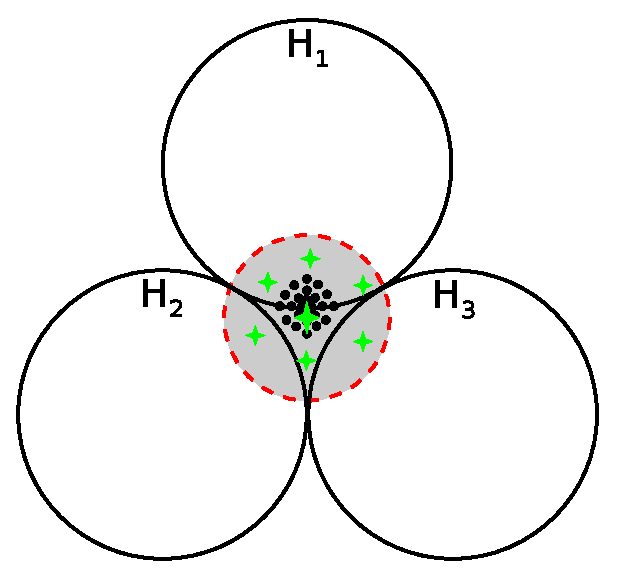
\includegraphics[width=.5\textwidth]{figs/blurring}}
  \caption{Gaussian Blurring to Fill Sparse Lattices.}\label{blurring}
\end{figure*}

Another way to overcome the hard-margins region assignments induced by a discrete lattice is to generate random points
in an $r/2$ radius around the projected vector.  This perturbation about the projected vector results in an approximate
probability density region around the data point.  In order to achieve an approximate radius probing in all dimensions,
we add a Gaussian vector having elements $\{n_1, n_2, ..., n_d\}\in R$, where $\|R\|\approx r$ and is composed of
elements $n \in N(0,r)$.

\subsection{Multi-Projection Re-Association}\label{occultationSection}

Re-association with the original vectors is used to recover the final centroids as shown in Figure \ref{lowtohigh}.
However, we must now resolve the common case where low dimensional representations of re-associated vectors are
unrelated to those of other projections.  A simple solution found in \cite{braverman} and in other streaming algorithms
is to merge the over-estimated centroid set in an off-line step such as weighted $k$-means.  The off-line step merges
the $k\times \text{number of projections}$ representations of candidate centroids but in the original dimensional
embedding.

\begin{figure}
    \centerline{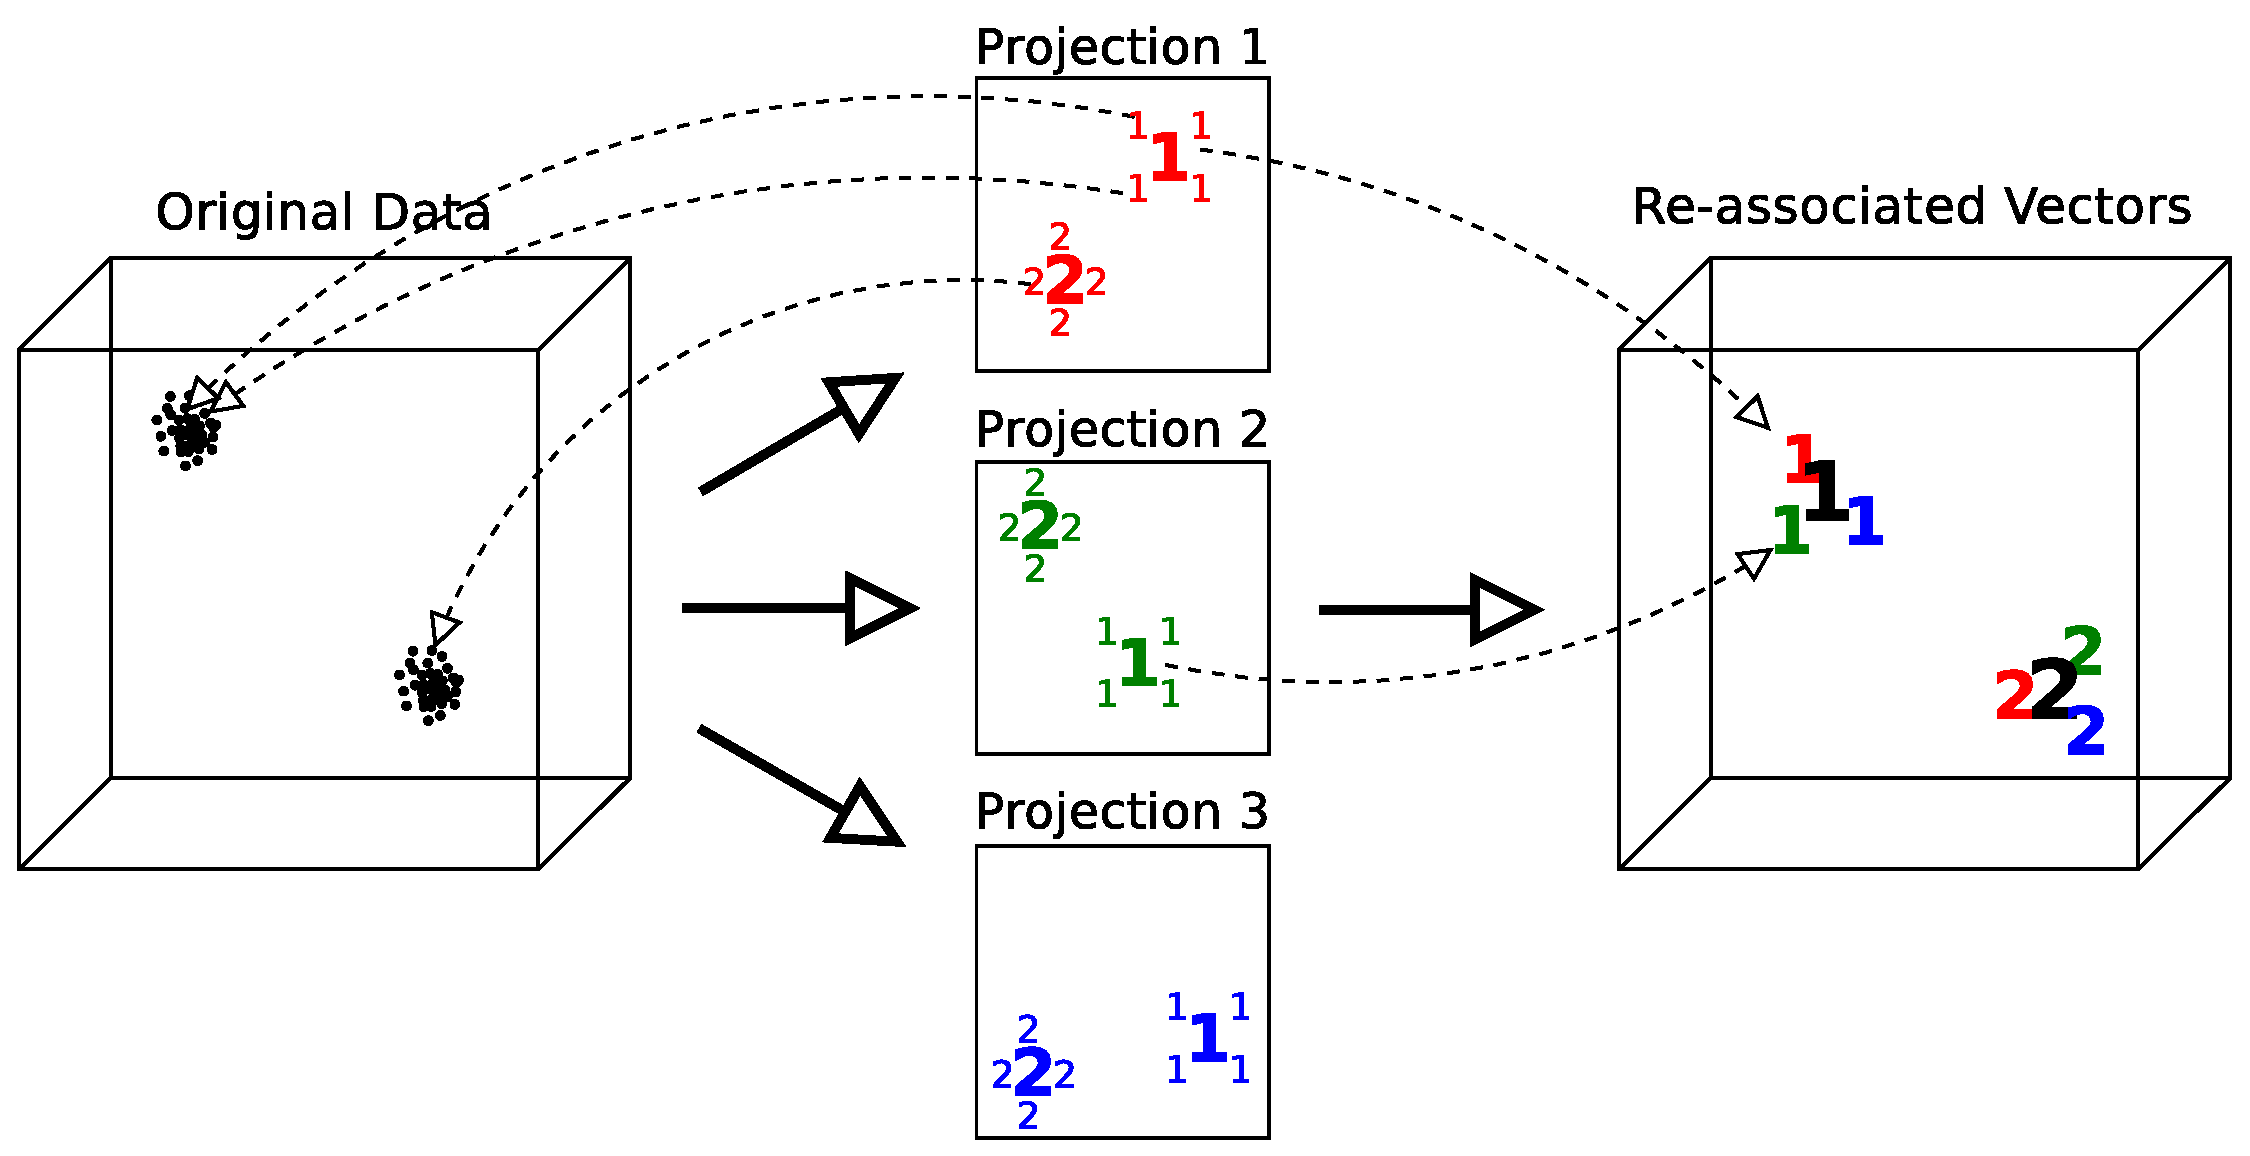
\includegraphics[width=.8\textwidth]{figs/LowToHigh}}
    \caption{Multiple projections $\mathbb{R}^{3}\rightarrow \mathbb{R}^2 \rightarrow \mathbb{R}^3$}\label{lowtohigh}
\end{figure}

A problem known as occultation arises when disjoint clusters in a $d$-dimensional space have non-disjoint projections on
lower-dimensional subspaces of $\mathbb{R}^d$.  Specifically, the probability of a $u$-occultation for the
$d$-dimensional space projected to 1-dimensional subspace is: $pr(u) = 1-{\frac{2}{\pi}} arcos({\frac{r_1+r_2}{d-c}})$,
where $r_1, r_2$ are radii of the respective clusters, and $d-c$ is the distance between them \cite{Urruty2007}.  The
method employed in \cite{Urruty2007} is to repeat the projection until a non-occulting projection is found.  The rate of
convergence for finding a non-occulting projection is given as:

$$\underset {d\rightarrow \infty}{lim}1-\bigg({\frac{2(r_1+r_2)} {\pi \|d-c\|}}\bigg)^d = 1$$ \label{occultation}

\noindent
which is exponential in $d$.  Recognized in \cite{Urruty2007}, this bound is slightly more favorable for an orthogonal
projection than the convergence rate of multiple single projections, as the distinct random projections are not always
linearly independent.  For certain decoders like the Leech Decoder and Spherical LSH, the required 24 and 32-dimensional 
projection is nearly orthogonal when the projection matrix is constructed of Gaussian random variables \cite{vempala}.


\RestyleAlgo{boxruled}
%%\begin{figure}[h]
%% \caption*{Data}
%%  $K$ - number of clusters\\
%%  $X=\{x_1,...,x_n\}$, $x_k \in \mathbb{R}^m$ - data vectors\\
%%  $ C$- a $k$-HH counter\\
%%  $\mathbb{H}$ - LSH Function\\
%%  $\mathbb{P} = \{p_1,...p_n\}$ - set of projection matrices\\
%%  $L=\{\{\varnothing\}...\}$\\
%%  $M = \{C,[0,...0]\}$\\
%%\end{figure}
%%\RestyleAlgo{boxruled}

\begin{algorithm}
\caption{ 2-Pass \textsf{RPHash} Algorithm\label{2passrp}}
\KwData{\ \\
  $K$ - number of clusters\\
  $X=\{x_1,...,x_n\}$, $x_k \in \mathbb{R}^m$ - data vectors\\
  $ C$- a $k$-HH counter\\
  $\mathbb{H}$ - LSH Function\\
  $\mathbb{P} = \{p_1,...p_n\}$ - set of projection matrices\\
  $L=\{\{\varnothing\}...\}$\\
  $M = \{C,[0,...0]\}$\\}

\ForAll{$x_k \in X$} 
{
  \ForAll{$p_i \in \mathbb{P}$} 
  {
    $\tilde{x_k}\leftarrow \sqrt{\frac{m}{d}}p_i^{\intercal}x_k $\\
    $t = \mathbb{H}(\tilde{x_k})$\\
    $L[k][i] = t$\\
    $C$.add($t$)\\
  }
}
\ForAll{$x_k \in X$}
{
  \ForAll{$c_i \in C$.top($K$)}
  {
    \If{$L[k] \cap M[i][0] \neq 0$}
    {
	$\Delta = M[k]-x_k$\\
	$M[k]=M[k]+\Delta/count$\\
	$L[k]$.add($M[i][0]$)\\
    }
  }
}
 \KwResult{$M$ }
\end{algorithm}

\begin{figure}
    \centerline{\includegraphics[width=.8\textwidth]{figs/rphashoverview}}
    \caption{Streaming \textsf{RPHash} Diagram}\label{rphash}
\end{figure}

In addition to Achlioptas efficient random projection method for databases, a further reduction in the number of
operation required for random subspace projection called the Fast Johnson-Lindenstrauss Transform (FJLT)
\cite{ailon2006,Dasgupta,ailon2013} is currently an active area of research.  FJLT, and similar nearly optimal
projection methods, utilize the local-global duality (Heisenberg Principle) of the Discrete Fourier Transform to
precondition the projection matrix resulting in a nearly optimal number of steps to compute an $\epsilon$-distortion
random projection \cite{ailon2006,Dasgupta,ailon2013}.  A sub-linear bound on the number of operations required for the
dominant projection operation may further improve \textsf{RPHash}'s overall runtime complexity.  However it only becomes
beneficial when the vector dimensionality $d$ is very large.  For many clustering problems, this level of dimensionality is 
uncommon.

%Centroids are computed as the means of the subsets of data vectors prior to
%projection, in each region.

%\subsection{Clustering on Streaming Data and Approximate $k$-Heavy Hitters}

%To perform RPHash on a streaming dataset, the itemset counter must be bounded and able to quickly
%respond to itemset support queries. Formally, the \textbf{$k$-Heavy Hitters}(\emph{$k$-HH}) problem
%is the problem of identifying the $k$ most frequent items in a dataset. It can trivially
%be solved using a histogram with $\theta(n)$ space.  In the case of streams, distributed
%and big data, the space requirements are potentially infinite making the histogram
%approach infeasible.  In \cite{alon1996} the related distinct counting problem for
%streams, is shown to require $\theta(n)$ in the worst case.  As with many cases involving
%unbounded memory requirements, approximate approaches have been proposed such as
%\cite{Karp,Morris,Manku}.  A thorough survey of approximate distinct item counting and
%algorithms can be found in \cite{Cormode} where counting algorithms are partitioned in to
%two categories: Count based and sketch based.
%\begin{figure}
%    \centerline{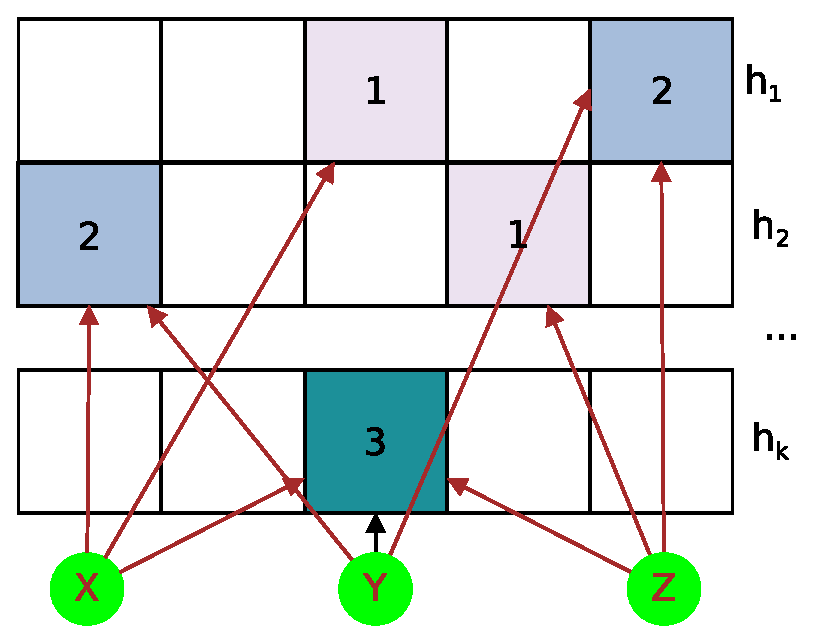
\includegraphics[width=.35\textwidth]{figs/countmin}}
%    \caption{Count-Min Sketch Algorithm}\label{countmin}
%\end{figure}
%One of the earliest streaming solutions for the approximate $k$-HH algorithms is the
%Count-min Sketch algorithm \cite{Cormode2}. Figure \ref{countmin} shows the primary data
%structure and action of the Count-min Sketch Algorithm for 3 elements $(X,Y,Z)$ and $k$
%hash functions.  Count-Min Sketch can be used to solve the approximate $k$-HH problem with
%only the additional of a priority queue using $\theta({1\over \epsilon} log {1 \over
%  \delta})$-space with error $(1-\epsilon)f$ where $f$ is the minimum frequency $m \over
%k$ to be consider frequent.

%Below we give the streaming version of the RPHash Algorithm. 

\subsection{Overview of \textsf{streamingRPHash}}

\textsf{streamingRPHash} is a stream clustering variant of the original 2-Phase \textsf{RPHash} algorithm of \cite{carraher-15}
which employs both approximate and randomized techniques to solve the $k$-means clustering problem.  To combat the curse
of dimensionality, \textsf{streamingRPHash} performs multi-probe, random projection with Gaussian blurring on high
dimensional data vectors \cite{Andoni}.

The general idea of \textsf{streamingRPHash} is motivated by a particular bad-case result in LSH based Nearest Neighbor
(LSH-NN) search where a single bucket contains an unprecedented number of candidate nearest neighbors.  This is a
problem in LSH-NN as the bucket then has to be linearly scanned for the optimal solution.  However, these degenerate
buckets can also be viewed as locally dense regions or density modes in the data.  Histograms offer a familiar 1-d
analog of our clustering solution.  A further advance of this considers not just the points within an arbitrary
histogram boundary, but relaxes the boundaries with a kernel based window function to smooth the overall population
density estimation.  A staple in kernel density estimation, the Parzen's window is a key motivation of the
\textsf{streamingRPHash} algorithm.

Due to the goal of providing an approximate solution to $\mathbb{R}^d$ for $d\gg1$, we must extend the windowing and
estimation techniques of Parzen's window to high dimensional space.  We could immediately apply the d-dimensional
hypercube partitioning and then count partition memberships.  But this method would suffer from many complexities
arising from the curse of dimensionality.  Similar to the issues encountered with k-d Tree NN \cite{marimont}, it will
also be computationally prohibitive and restricted by memory limitations.  \textsf{streamingRPHash} offers to mitigate
these issues by optimizing the approximate solution instead of the exact.

\textsf{streamingRPHash}, being motivated in part by LSH-NN, uses locality sensitive hash functions to partition the
data space evenly.  After both accuracy and time complexity tests, the 32-orthoplex spherical hash function was found to
be optimal across a wide range of datasets and system configurations.

An outline of the steps in the \textsf{streamingRPHash} algorithm are discussed below and summarized in Algorithm
\ref{streamingRPHashAlg}.  Some of the aspects of its function in regards to randomness and approximation are
highlighted here.  First, we discuss the generative nature of its region assignment.  Dense regions are identified by decoding data vectors
using a set of LSH functions.  In general the problem space will not match the locality sensitive hashing subspace.  The
previously described Johnson-Lindenstrauss (\emph{JL}) lemma offers a solution to this problem at the cost of a matrix
vector product.  Although \emph{JL}-lemma requires an $m\times d$ matrix of Gaussian random variables be formed,
\cite{Achlioptas01} suggests an approximate method to form the random projection matrix whose elements
$r_{ij}\in\textbf{R}$ have values from $\{1, 0, -1\}$ with probabilities $\{\frac{1}{6}, \frac{2}{3}, \frac{1}{6}\}$
respectively.  A further computational reduction is then achieved by treating the matrix-vector product as a linear scan
over the non-zero elements of the projection matrix, allowing us to effectively skip $\frac{2}{3}$ of the projection
computation, with the remaining $\frac{1}{3}$ operations consisting only of scalar additions.  Following this
computation, a scaling factor of ${\frac{1}{\sqrt{n}}}$ is also needed to preserve approximate distances between
projected vectors.

The subspace spanned by the 32-orthoplex is well below the requirements suggested by the \emph{JL}-bound for individual
vector discrepancy.  Fortunately, the effectiveness of projected $k$-means has been demonstrated successfully for
projections well below the \emph{JL}-bound (and well below $d = 32$) \cite{bartal,bingham}.  However, internal tests
show precision-recall performance drops as projection space dimensionality decreases.  To boost the overall data
retention of our clustering, we opt to perform multiple projections on original data vectors, followed by a
reconstruction step.  Similarly, a `blurring' step is used to increase the overall hash collision rate for nearby
vectors.  \textsf{streamingRPHash} `blurs' the projected data by applying shifts to projected vectors which help to
overcome the hard margins of the LSH decoder.

\section{\textsf{streamingRPHash} Algorithm} 

\textsf{streamingRPHash} follows the same structure as the original \textsf{RPHash} algorithm such as multiple random subspace
projections and their Re-Associations, Gaussian Blurring and LSH Functions.  However, the difference is in the way in
which \textsf{streamingRPHash} identifies and updates frequent density modes.  Due to the streaming data model's requirements
that an incoming data stream cannot be randomly accessed, or completely stored, we can only store a sketch of the
incoming data.  Furthermore, \textsf{streamingRPHash} cannot store the entire dataset, so the set of candidate centroids must be
bounded.  Fortunately, the Count-Min Sketch and its $k$-HH implementation fulfill both of these requirements.
The sequential version of the \textsf{streamingRPHash} algorithm is given in Algorithm \ref{streamingRPHashAlg}.

\begin{algorithm}
\RestyleAlgo{boxruled}
\KwData{\ \\
  $k$ - number of clusters\\
  $X=\{x_1,...,x_n\}$, $x_i \in \mathbb{R}^m$ - data vectors\\
  $M$- lsh\_key $\rightarrow$ centroid map \\
  $C$- cm-sketch data structure \\
  $T$- CM-Sketch based $\epsilon k$ bounded priority queue\\
    $R= \{r_1,...,r_{\log_2d}\}$, $r_i \in \mathbb{R}^d$ - Gaussian blurring vectors\\
  $\mathbb{H}(\cdot)$ - LSH Function\\
  $\mathbb{P} = \{p_1,...p_n\}$ - set of $n, m \times d $ projection matrices w/ \emph{JL} property\\}
\RestyleAlgo{boxruled}

\caption{\textsf{streamingRPHash} Algorithm\label{streamingRPHashAlg}}
\DontPrintSemicolon
\ForAll{$x \in X$} 
{
  \ForAll{$p \in \mathbb{P}$} 
  {
    $\tilde{x}:= \sqrt{\frac{m}{d}}p^{\intercal}x$ \tcp*{Random Projection}
    \ForAll{$r \in R$} 
      {
      $t := \mathbb{H}(\tilde{x}+r)$ \tcp*{LSH Hashing}
      $C$.add$(t)$\\
      \eIf{$t\in M$.keys}
      {
	$M[t].wadd(x)$  \tcp*{Weighted add}
      }
      {
	 $M[t]=$new centroid($x$,C.count(t))\\
	 $T$.insert$(M[t])$\\
      }
      M.remove(T.pop())  \tcp*{remove least}
    }
  }
}
\KwResult{OfflineWeightedClusterer($M$.items)}
\end{algorithm}

%% According to the \emph{JL} lemma, the sub-projections will conserve the pairwise
%% distances in the projected space for points with $\epsilon$-distortion in which the
%% size of the dataset is proportional to the logarithm of the number of dimensions in the
%% randomly projected subspace.  In addition to compressing a dataset to a computationally
%% more feasible subspace for performing space quantization, random projection can also
%% make \emph{eccentric} cluster more spherical \cite{Dasgupta2000,vempala}.

%The lattice decoder implementation relies on the decomposition of the binary $(24,22,8)$
%extended Golay Code into 4 partitions of the $(6,3,4)$ quaternary hexacode and its
%relation to the Leech Lattice as a type B lattice construction.  This decomposition and
%relation to the Golay Code provides a real worse case decoding complexity well below the
%asymptotically exponential bound for trellis decoders as the dimension $d$ increases
%\cite{Tarokh1,Tarokh2}.  The Leech lattice is a unique lattice in 24 dimensional space
%with many exceptional properties, however, of importance to \textsf{streamingRPHash} is
%that it is the densest regular lattice possible in 24 dimensions and nearly optimal among
%theoretical non-regular packings \cite{Cohn}.  The 24 dimensional subspace partitioned by
%the Leech Lattice is small enough to exhibit the spherical clustering benefit of random
%projection.  Low distortion random embeddings are also feasible for very large dataset
%($n = \Omega(c^{24})$) objects while avoiding the occultation phenomena
%\cite{Urruty2007}.  Furthermore, the decoding of the Leech lattice is a well studied
%subject, with a constant worse case decoding complexity of 331 operations \cite{Vardy95}.
%In addition to the Leech Lattice, other space quantizers exist with even better cr-NN
%performance for special types of spherically distributed data and the cosine distance.  A
%partitioning scheme of \cite{SLSH} uses the hypersphere surface partitioning of inscribed
%regular polytopes.  Although a variety of n-dimension regular polytope constructions
%exist, we choose the n-orthoplex for its simplicity, and relatively low number of
%partition regions ($2d$, compared to hypercube and simplex).  Furthermore, random
%rotations of the hypercube are used to generalize the partitioning, and on projected
%data, are already present in the projection matrix.

%Centroids are computed as the means of the subsets of data vectors prior to projection,
%in each region.  The approximation of a random projection matrix is not only
%computationally more efficient to generate, it also requires $frac{2}{3}$ fewer
%operations during the projection process., and unlike a projection matrix formed from
%truly Gaussian random variables, has an even better probability of yielding a positive
%semi-definite projection matrix at lower dimensions.

\section{$k$-HH}{Streaming Data and Approximate $k$-Heavy Hitters}

To apply \textsf{streamingRPHash} to data streams, the candidate centroid set must be bounded and able to quickly
respond to most frequent itemset queries.  Formally, the $k$-Heavy Hitters (\emph{$k$-HH}) problem is the problem of
identifying the $k$ most frequent items in a dataset \cite{cormode}.  It can trivially be solved using a histogram with
$\theta(n)$ space.  In the case of data streams, space requirements are potentially unbounded, making the histogram
approach infeasible.  In \cite{alon1996}, the related distinct counting problem for streams is shown to require
$\theta(n)$ space in the worst case.  As with many cases involving unbounded memory requirements, approximate approaches
have been proposed such as \cite{karp-03,morris-78,Manku}.  A thorough survey of approximate distinct item counting can
be found in \cite{cormode3} where counting algorithms are divided into two categories: \emph{count based} and
\emph{sketch based}.

One of the earliest streaming solutions for the approximate \emph{$k$-HH} algorithms is the Count-Min Sketch data
structure \cite{cormode2}.  Figure \ref{countmin} shows the primary data structure for 3 elements $(X,Y,Z)$ and $k$ hash
functions.  Count-Min sketch can be used to solve the approximate \emph{$k$-HH} problem with only the addition of a
priority queue using $\theta({1\over \epsilon} log {1 \over \delta})$ space with error $(1-\epsilon)f$, where $f$ is the
minimum frequency $m \over k$ to be considered frequent.

%\RestyleAlgo{boxruled}
%\begin{figure}[h]
% \caption*{Data}
%  $K$ - number of clusters\\
%  $X=\{x_1,...,x_n\}$, $x_k \in \mathbb{R}^m$ - data vectors\\
%  $ C$- a $k$-HH counter\\
%  $\mathbb{H}$ - LSH Function\\
%  $\mathbb{P} = \{p_1,...p_n\}$ - set of projection matrices\\
%  $L=\{\{\varnothing\}...\}$\\
%  $M = \{C,[0,...0]\}$\\
%  $r = \{r_0,...,r_{24}\}$ - random blur vector $\in \mathbb{R}^{24}$ \\
%\end{figure}
%\RestyleAlgo{boxruled}

%\begin{algorithm}
%\caption{Streaming Algorithm\label{streamingRPHashAlg}}
%\ForAll{$x_k \in X$} 
%{
%  \ForAll{$p_i \in \mathbb{P}$} 
%  {
%    \For{$b \in {{1}\over{D(\Lambda)}}$} 
%      {
%      $\tilde{x_k}\leftarrow \sqrt{\frac{m}{d}}p_i^{\intercal}x_k $\\
%      $t = \mathbb{H}(\tilde{x_k}+r)$\\
%      $tmp \rightarrow C$.top($K$).get($[t,x_k,0]$)\\
%      \eIf{tmp $\neq \varnothing$}
%      {
%	  $\Delta\leftarrow tmp[1]-x_k$\\
%	  $tmp[2]\leftarrow tmp[2]+1$\\
%	  $tmp[1]\leftarrow tmp[1] + \Delta/tmp[2]$\\
%      }
%      {
%	  $C$.add($[t,x_k,1]$)\\
%      }
%    }
%  }
%}
%\KwResult{$C$.top($K$)}
%\end{algorithm}

While the code base for \textsf{streamingRPHash} contains implementations for several LSH methods (including $E_8$,
Leech, and Spherical), our experimental studies show that the best overall performance is achieved with Spherical.
Hence the experiments in this dissertation report results with the spherical 32-orthoplex decoder of \cite{SLSH}.  The
spherical orthoplex decoding consists of a projection to 32$d$ space followed by a vector normalization step in order to
have the vector lie on the surface of a hypersphere.  Next, a random rotation is applied to the 64 basis vectors of the
32-orthoplex.  The basis vector nearest to the projected vector is then used as the vector's representative, and the
corresponding bits resulting from the natural ordering of basis vectors are used to define a $log_2(64)$ partial
decoding.  Subsequently, two similar additional hashings are applied to generate a total 18 bits of entropy.

%\RestyleAlgo{boxruled}
%\begin{algorithm}
%\caption{Streaming Algorithm\label{streamingRPHashAlg}}
%\ForAll{$x_k \in X$} 
%{
%  \ForAll{$p_i \in \mathbb{P}$} 
%  {
%    \For{$b \in {{1}\over{D(\Lambda)}}$} 
%      {
%      $\tilde{x_k}\leftarrow \sqrt{\frac{m}{d}}p_i^{\intercal}x_k $\\
%      $t = \mathbb{H}(\tilde{x_k})$\\
%      $tmp \rightarrow C$.top($K$).get($[t,x_k,0]$)\\
%      \eIf{tmp $\neq \varnothing$}
%      {
%	  $\Delta\leftarrow tmp[1]-x_k$\\
%	  $tmp[2]\leftarrow tmp[2]+1$\\
%	  $tmp[1]\leftarrow tmp[1] + \Delta/tmp[2]$\\
%      }
%      {
%	  $C$.add($[t,x_k,1]$)\\
%      }
%    }
%  }
%}
%\KwResult{$C$.top($K$)}
%\end{algorithm}

\section{Data Security}{Data Security: At no added cost}\label{security}

Recent United States government initiatives pushing for the large scale availability of data resources have made vast
quantities of de-identified health information available to the public.  These resources however have prompted advances
in attacks on de-identification of whole genome sequence data.  Such attacks have been used to associate, thought to be,
anonymous medical records with specific individuals \cite{deident}.  Similar de-anonymization attacks
\cite{deanon1,deanon2} along with a presidential commission (privacy and progress in WGS) have prompted a need for
better data security of medical records data.  The \textsf{RPHash} algorithm provides an intrinsic solution to this
problem in both the distribution of data among servers as well as during the communication steps required by the
algorithm.

While attempting to mitigate communication restrictions, \textsf{RPHash} intrinsically provides some security in the data
it exchanges.  Previous attempts at securing data in distributed systems required additional cryptographic steps
\cite{Lindell2000}.  Namely, the randomly projected centroid IDs, and the aggregation of only the $k$-largest cardinality
vector sets.  Non-distributed data clustering requires the entire dataset to reside on the processing system and
distributed methods often require communication of full data records between nodes.

In the subspace projection step of \textsf{RPHash}, nearly-orthogonal random projection is utilized as a destructive
operation, providing vector anonymity.  As a consequence of projecting the real data vectors to a random subspace via a
near, but not completely orthogonal matrix, destructive data loss occurs providing a cryptographic ``trapdoor''
function.  The data loss is an intrinsic part of the \textsf{RPHash} clustering algorithm that has little adverse effect
on its model generation and subsequent recall accuracy.  Given the likelihood that \textsf{RPHash} is applied to a dataset where
the number of vectors $n$ is much greater than the desired $k$ centroids, recovering an individual's private information
would require knowledge of $\frac{n}{k}$ (on average) records in the representative centroid.

\section{Software Implementation Details}

%% LEE: not really necessary and since it's just one paragraph, it's not a proper paragraph.  alternatively you could
%% expand it to multiple sentences and document the repos where everything lies.

%% RPHash and Variants of RPHash are provided in a variety of languages (Go, Python, and Java), however the primary
%% testing and performance analysis is performed on the Java variant.

%% LEE: is the abstaction from the abstract object \texttt{AbstractClusterer} or something else??  also, is it an
%% absract function or an abstract class??  please cleanup and check the names/capitalization of everything in the next
%% paragraph.  i tend to set references to code names in typewriter font.

\textsf{RPHash} and Variants of \textsf{RPHash} are provided in a variety of languages (Go, Python, and Java), however the primary
testing and development is done on the Java variant.  All software development and collaboration was
tracked using the git version control system and is made available on-line: 
\begin{itemize}
\item \url{https://github.com/wilseypa/rphash-java}
\item \url{https://github.com/wilseypa/rphash-spark}
\item \url{https://github.com/wilseypa/rphash-golang}
\item \url{https://github.com/leecarraher/PyRecRPHash}
\end{itemize}

The \textsf{RPHash} test frameworks is designed in \texttt{java} following an object-oriented approach.  Additional
performance metrics and algorithms for comparison are provided by various Matlab packages.
Common functional units with the similar functions are designed as implementations of general abstract classes (i.e 
\texttt{ArrayList} implements \texttt{List} functions)
Examples of abstract functional units that are described in more detail are \texttt{AbstractProjector},
\texttt{AbstractClusterer} , \texttt{AbstractDecoder}, and \texttt{AbstractCounter}.  The methods contained in each interface
pertain to their function within the \textsf{RPHash} \texttt{java} Framework.

The abstract class of all \textsf{RPHash} variants, which includes other clusterers for comparison is the \texttt{AbstractClusterer} class.
For algorithms specific to streaming datasets, a further abstraction of the \texttt{AbstactCluster} method is provided, \texttt{StreamingClusterer}
which amends the abstract clusterer with function prototypes for adding vectors in a stream and invoking the off-line process.  Implementing
clusterers in this framework allows us to easily design tests that are applicable to all \textsf{RPHash} variants and other clustering algorithms.

For implementation of the offline clustering and post processing clustering steps, multiple standard clustering
algorithms were implemented. These methods all implement the \texttt{AbstractClusterer} interface.  
In particular the following offline algorithms are included in the code base: Hartigan and
Wong $k$-Means \cite{Hartigan}, agglomerative clustering with single, complete average, and wards method link strategies,
Mean-Shift \cite{comaniciu-02}, Maximum Likelihood \cite{Hathaway}, DBScan \cite{dbscan}, $k$-Means++ \cite{arthur-07}, Braverman
\emph{et al} Streaming $k$-Means \cite{braverman} , Ailon \emph{et al} Streaming $k$-Means \cite{streamkmeans}, as well as a
dummy clusterer that simply samples the dataset.  All clustering methods can be wrapped in a multi-reseeding method that
optimizes within-cluster sum of squared error.

Multiple LSH algorithms were implemented for testing and comparison as implementations of the \texttt{AbstractDecoder} class. Decoders include 
the P-Stable-Distribution Decoder \cite{datar-04},
Spherical LSH Decoder \cite{SLSH}, Leech Decoder \cite{Andoni06,Amrani}, $E_8$ Decoder \cite{SPLAG}, the classic Dihedral Group Decoder\cite{SPLAG}, 
Origin Hamming Decoder \cite{indyk-98}, Binary Golay Decoder \cite{Amrani}, and or proposed Depth Probing Decoder.  All Decoders are composable into
multi-level decoders, through implementation of the multi-decoder wrapper.

\texttt{AbstractProjectors} consist of the DB-Friendly random projection method of \cite{Achlioptas01}, a the Gaussian variate based
projection \cite{vempala}, a bitwise DB-Friendly random projection method, the Fast
Johnson-Lindenstauss Transform \cite{ailon2006}, and the classic Principle Component projection.  

A set of counting and sketching
algorithms are also implemented in the \textsf{RPHash} test framework and are implementations of the \texttt{AbstractCounter} class.  
The included counting algorithms are: the Count-Min sketch \cite{cormode},
and its $k$-Heavy Hitter implementation \cite{cormode2}, Lossy counting \cite{morris-78} and a hash table based exact counter.  The
Count-Min implementation is adapted to also support vector sums and decay rates for streaming data in which clusters are regarded as
temporal structures.

For testing \textsf{RPHash}, a framework of statistical performance metrics and data generators and readers is provided.  The
generators consist mainly of Gaussian cluster generators, that can be sparse, heteroscedastic, and full or streaming.
All data readers implement a simple matrix format that supports both binary and ASCII data with uncompressed and LZ
compressed data.


\include{05.5adaptivelsh}

\chapter{Performance Analysis}\label{performance}

\textsf{RPHash} performance is tested against a selection of standard and state-of-the-art algorithms for
clustering at rest and streaming data.  The goal of our performance analysis is to provide
comparable clustering performance to standard and state-of-the-art algorithms, while showcasing
\textsf{RPHash}'s processing speed compared to other algorithms.  Due to the ill-posed nature of the
clustering problem, we provide evaluation over a set of clustering metrics in an attempt to capture
the multifaceted nature of what 'good' clustering is.

Due to the dependence between \textsf{RPHash} clustering and timing performance with \textsf{RPHash} components
configuration, we first perform an evaluation of component dependence and performance.  We then
choose the optimal configuration, based on speed, data set stability, and clustering performance, as
a baseline configuration for all subsequent \textsf{RPHash} experiments.

Our clustering comparison approach consists of sets of experiments where our clustering method is
compared to various common clustering methods.  The compared clustering methods vary by which \textsf{RPHash}
variant we are evaluating and its intended data access structure.  For our two pass algorithm, we
consider other algorithms that require a finite number of passes over the data, with sub polynomial
memory growth complexity.  Likewise, for streaming data, we compare our streaming algorithm with
other streaming clustering algorithms that have sub polynomial processing complexity, and sub linear
memory growth.  Therefore, the performance analysis discussion of the three \textsf{RPHash} algorithms will
be given in three parts.  Each section will define the comparison algorithms, and the corresponding
data source setting, as well as any other pertinent experiment specifics.

The remainder of this chapter is organized as follows.  First we describe our experimental model,
data sources, test structure, metrics, and comparison algorithms.  Next we provide the parameter
exploration study, to establish our baseline configuration.  The third and fourth section comprise
the main performance results for the two pass \textsf{RPHash} algorithm.  The following section shows results
specific to the \textsf{streamingRPHash} algorithm, and streaming data.  Followed by an evaluation
of the Tree-Walk RPHash \textsf{TWRP} Algorithm.  Lastly we give an overview of the $k$-anonymity security
performance of random vector projection in \textsf{RPHash}.

%% 1. description of the test models and synthetic generation tool and setup thereof
%% 2. the parameter exploration of RPHash (because i assume you'll then do most of you testing with only a few of the
%%    best configurations
%% 3. tests with real data
%% 4. tests with synthetic data for (an some organized order: noise, scalability (of parallelism), scalability on total
%%    vectors, scalabilty on dimensions
%% 5. streamingRPHash test results
%% 6. adaptive LSH based RPHash (if you intend to show these separately.
%% 7. TRWP results

\section{Metrics and Data Sources}

The \textsf{RPHash} framework provides a comprehensive experimental framework consisting of evaluation metrics
and data generation procedures.  Both real world and synthetic data sources are made available in
the testing framework.  The general test setup consists of data generation or ingest, into a static
memory resident array.  The vectors in the array are then randomized, to remove sample sequence
order dependence and clustering is performed, on the data.  The results of the clustering procedure
are then evaluated against applicable clustering metrics.  Due to the randomized nature of \textsf{RPHash}
and many clustering algorithms, all experiments are performed 6 times to establish an average
performance and variance over the applicable metrics.  The system provisioned for experimentation
was stable, and as such outliers were not removed.  The details of the various aspect of our
experimental set up follow.

\subsection{Real World Data}

\textsf{RPHash} is a general clustering algorithm intended for a range of high dimensional clustering
problems.  We designed experiments around a variety of real world datasets.  To assess the
clustering performance of \textsf{RPHash}, a set of expert labeled, real world data sets used throughout the
our performance experiments is summarized in Table \ref{realworld}.  Labeled datasets are useful
for computing external metrics on clustering performance, however the labeling requirement is often
infeasible for very large datasets.  As a result, we have included a common dataset for this
purpose, based on the Word2Vec transformation of semantic data \cite{word2vec}.  As well as a
dataset to test anonymization, the MIMIC II dataset \cite{MIMICII}.

Table \ref{realworld} gives and overview of the features found in these labeled datasets and will be
referenced throughout the remainder of this chapter. The two most common datasets featured in our
tests are the human activity and location based datasets.  The first dataset of these activity
datasets is the \emph{Human Activity Recognition Using Smartphones} \cite{har}.  It has 10,299
records (the first 10,000 are used in this study), and 561 attributes representing time and
frequency domain variables.  The dataset contains six clusters which denote the six activities
(WALKING, WALKING\_UPSTAIRS, WALKING\_DOWNSTAIRS, SITTING, STANDING, LAYING) performed by each
person. Next we have the \emph{Indoor Localization} dataset based on device WiFi location.
(\url{https://archive.ics.uci.edu/ml/datasets/UJIIndoorLoc}) \cite{UJII}.  It is a multi-building
multi-floor indoor localization database to test Indoor Positioning System that rely on WLAN/WiFi
fingerprint.  The dataset has a total of 21,048 vectors.  This study uses first 21,000 vectors each
having 520 attributes which represent WiFi fingerprints composed of 520 intensity values detected by
Wireless Access Points.  Building ID is used as the target variable which has three possible values.
Three citation and link datasets are included: WebKB (Wisconsin) Dataset \cite{sen-08}, Cora Dataset
\cite{sen-08}, and CiteSeer Dataset \cite{sen-08}.  These datasets consist of the sparse citation
graphs of text corpus.  In each, documents are organized into a set of sub-corpus clusters.
CNAE-9 \cite{cnae} contains natural language data represented by a sparse term-document matrix.  The
Arrhythmia \cite{guvenir-xx} contains dense signal measurements of ECG data grouped into arrhythmia
and regular heart rhythm.

\begin{table*}
\centering
\begin{tabular}{|l|r|r|r|l|}
\hline
\rowcolor[HTML]{FFCE93} 
\textbf{Data Set} & \textbf{Num of}   & \textbf{Num of}   & \textbf{Num of} & \textbf{Type of} \\
\rowcolor[HTML]{FFCE93}
                  & \textbf{Clusters} & \textbf{Features} & \textbf{Vectors} & \textbf{Data} \\ \hline
Arrhythmia \cite{guvenir-xx}     & 16 &  279 &   452 & Real   \\
CNAE-9 \cite{ciarelli-xx}        &  9 &  856 &  1080 & Binary \\
Cora \cite{sen-08}               &  7 & 1433 &  2708 & Binary \\
Gisette \cite{guyon-04}          &  2 & 5000 &  7000 & Real   \\
Human Activity \cite{anguita-13} &  6 &  561 & 10299 & Real   \\
UJIIndoorLoc \cite{sospedra-14}  &  3 &  520 & 21000 & Real   \\
WebKB \cite{sen-08}              &  5 & 1703 &   265 & Binary \\ \hline
\end{tabular}
\caption{Real-World Data Sets.}\label{realworld}
\end{table*}

In addition to our standard labeled datasets, we also include some large unlabeled datasets.  The
first dataset utilizes the popular word2vec \cite{word2vec} space representations of topic vectors.
The dataset Google Word2Vec News dataset \cite{googlenews} is a very large publicly available
dataset built from articles in the Google news corpus.  It contains 300k topics represented as 300
word2vec attributes.  Our next large, unlabeled dataset is the medical dataset MIMIC II
\cite{MIMICII} biometric dataset.  We pre-process this dataset, prior to clustering by taking
generating signatures of the biometric markers ``RESP", ``ABP", ``ECG II" and ``PLETH".  The
signatures were created by taking the 64 most prevalent frequencies as identified via power spectral
density estimation of the signals. The dataset consists of 100,000 patient time based signals, and
is over 4 TeraBytes in total size.  Due to the rather large size, we sampled 38 full signal
observations from the 100,000 observations.

\subsection{Data Generators}\label{synth_data}

In addition to real world data, synthetic data generators are a major part of our test framework.
While real world datasets provide a realistic view of clustering performance, they are not very
useful in providing scalability and variability results over ranges of values.  We have implemented
both streaming and static data sources generators in the \textsf{RPHash} testing framework.

Our general vector stream consists of a user defined set of cluster centroids consisting of uniform
variates in the range $(-1,1)$.  The centroids however are not present in the data set, and merely
establish a ground truth mean around which synthetic vectors are generated.  Test vectors are
generated with equal probability of choosing any of the $k$ ground truth centroids and adding a
vector of dimensionally scaled Normal variates.  While this data source is well suited for
evaluating timing performance, the predictable structure of the data, is not very realistic and may
favors certain clustering methods over others.  To overcome these limitation, we provide a set of
configuration variables.

First, we must accept that equi-probable cluster membership is unlikely.  In many machine learning
problems, learning unlikely classes is more important than evenly partitioning data, such would be
the case in cancer screening, and Internet anomaly detection.  To provide this, we allow for a
non-equi-probable cluster centroid selection for the generation set.  Next we consider the
possibility for non-univariate data.  In real world data sets, clusters often have varying size and
shape.  While we maintain a requirement of generating ellipsoidal clusters, our test framework can
generate clusters with variable variance, by replacing the normal variate constraint, with a
Gaussian variate with variance chosen uniformly in the range $(0,1]/d$.  Another important aspect
  of real world data, not present in the described framework, is noise.  Again we provide this
  aspect, through a configurable noise percentage parameter.

In addition to the static data generation, we also provide a streaming data generator.  All
configuration parameters of the static data generation are available in the streaming version.  The
only difference is that vectors are generated one at a time, and are not stored.  This prevents us
from performing some clustering metrics, but it allows us to simulate the important unbounded nature
of streaming data sources.

A generator in the R programming language was also developed to access various R language based
streaming clustering algorithms.  The generator uses a similar technique as \textsf{DSD\_Gaussian}
function from the `stream' package to generate vectors from a random cluster in a continuous data
stream.

\subsection{Evaluation Metrics}\label{evalmetrics}

The clustering problem is an ill-posed machine learning problem.  While the $k$-Means problem
description establishes inter-cluster variance as the optimization metric, it may not be well suited
for many real world problems in which noise is present, or cluster shape is erratic.  For this reason
we provide a selection of clustering metrics that describe the 'goodness' of clustering both
internally and externally.

Internal metrics are metrics that can be computed directly from the data with no known ground truth,
while external metrics require cluster class labels, to compute. First we describe our internal cluster
metrics.  The most common internal metric for clustering,
established by the $k$-Means problem, is the within-cluster sum of squared errors (WCSSE).  This
metric establishes a value of inter-cluster vector similarity.  Formally, the WCSSE is:
$$
\text{WCSSE}(C) = {\overset{k}{\underset{i=1}{\sum}}} {\underset{x\in C}{\sum}}
||x-\mu_i||^2
$$
where $\mu$ is the mean value of each vector.  WCSSE is a useful metric for evaluating clustering
in which all of the vectors being clustered, are close to the mean of the cluster (compact).

Another internally calculable metric, similar to WCSSE, and the goal of $k$-means clustering is
the Silhouette Index.  Silhouette Index is less susceptible to the potential problems that WCSSE
might encounter if true clusters, are not compact.  Silhouette Index evaluates the ratio of
inter-cluster co-similarity to the nearest intra-cluster dissimilarity.  Silhouette Index includes the
WCSSE, but attempts to remove the impact of wide clusters, by taking the ratio of true WCSSE with
the false WCSSE of the nearest cluster centroid for a sample.

The Dunn Index (DI) is an internal clustering metric similar to the Silhouette Index and WCSSE.  DI
takes a blended approach toward cluster evaluation that favors tightly packed clusters that are far
from other nearby clusters.  The Dunn index is a ratio of the greatest inter-cluster distance between
two vectors in a cluster over the intra-cluster distance between the two closest clusters.

Both of these internal clustering metrics rely on a 'useful' (see \ref{rpprelim}) distance metric.
However, we are concerned more with high dimensional clustering problems in which the distance
metric may not be very useful.  For these types of problems, we rely on having some expert labeled
ground truth.  For the case of synthetic sets, this can be the centroid generator's centroids.  For
real world datasets, this is often expert labeled data.  Cluster purity is a clustering metric that
takes a supervised machine learning approach to evaluating cluster membership.  Cluster purity
measures the amount of correctly labeled clusters for a given partitioning.  More specifically it is
the sum of counts of correctly classified vectors in each cluster.
$$
\text{Purity}(C) = {{1}\over{N}}{\underset{c\in C}{\sum}} \underset{x\in X}{max} |c \cap x_j |
$$

A direct shortcoming of all of the above metrics is that they do not directly penalize
misclassification.  The Rand Index (RI) overcomes this shortcoming by establishing a ratio of
true-positive co-occurrence, false-positive co-occurrence, true-negative co-occurrence and
false-negative co-occurrence.  The ratio can be expressed without the false-positive and
false-negative values, by scaling it over the binomial coefficient of all possible pairs
$\binom{n}{2}$.  This ratio results in very small values for large datasets, so in practice, the
Adjusted Rand Index (ARI) is often used.  ARI scales the final ratio by the maximum ARI from the
mean ARI.  Formally, this computation is:
$$
\text{ARI}(C) = {{RI(C) - \mathbb{E}(RI(C))} \over {max(RI(C)) - \mathbb{E}(_RI(C))}}\\
$$

Variation of Information (VI) is another performance metric considered.  VI is an external metric
that measures the degree of correspondence between the clustering labeling and the ground truth
labeling.  It is similar to mutual information between two random variables.

Finally, timing and memory usage metrics are also included in performance tests.  Timing is
evaluated as the time delta between the start of vector processing, and the final centroid
generation.  Setup time, such as VM initialization or R startup, was not included in the timing
delta.  Timing is provided by the system clock, for the given machine, and averaged over six
experiments.

\subsection{Comparison Algorithm Details}

To evaluate \textsf{RPHash} Performance on static datasets we provide comparative performance data with the
following common clustering algorithms:
\begin{itemize}
 \item \textbf{$k$-Means:} It is implemented with 'kmeans' in R \cite{Hartigan}.\label{clusteralgos} 
 \item \textbf{Four methods of Agglomerative Hierarchical clustering:} Single Linkage, Complete
   Linkage, Average Linkage and Ward's minimum variance method.  At each stage distances between
   clusters are recomputed by the Lance-Williams dissimilarity update formula according to the
   particular clustering method being used.  Ward's (1963) clustering criterion, where the
   dissimilarities are squared before cluster updating, is used in the implementation of Ward's
   method (Murtagh and Legendre 2014).  All of these agglomerative clustering methods are implemented
   with 'hclust' in R.
\item \textbf{Self-organizing Tree Algorithm (SOTA):} It is implemented with 'sota' (Package
  'clValid') in R \cite{Herrero}.
\item \textbf{$k$-Means++} is implemented as the Hartigan and Wong \cite{Hartigan} implementation of
  $k$-Means, with random initial seeding based on the furthest from a vector metric defined in
  \cite{arthur-07}.  The version used in this comparison comes from the Apache Math library
  (\url{http://commons.apache.org/proper/commons-math/}).
\end{itemize}

For the streaming version of \textsf{RPHash}, we also include a selection of streaming clustering algorithms
for comparison.  In particular we provide comparative performance results to the following
algorithms: 

\label{streamingalgos}
\begin{itemize}
 \item \textbf{Streaming $k$-Means:} clustering algorithm for streams based on facility location
   problem \cite{braverman}.  Implementation from S-Space \cite{sspace}.
 \item \textbf{Damped Sliding Window:} \cite{zhu} window length $=100$.
 \item \textbf{DStream:} \cite{dstream} The size of grid cells is set at 0.8.
 \item \textbf{Biased Reservoir Sampling:} \cite{ccaggarwal} With a window length $=100$. 
\end{itemize}

\noindent
These algorithms are chosen because of their importance and availability (except for streaming
$k$-means) in the R statistical computing framework.  All of these algorithms follow the
conventional two-stage (on-line/off-line) approach for data stream clustering.  The weighted
$k$-means implementation of Hartigan and Wong (with $nstart = 25$ for algorithms implemented in R)
is used in the off-line stage.

\section{Parameter Exploration}\label{optimalconf}

In order to find the optimal configuration of \textsf{RPHash} over various synthetic and real world datasets,
we performed an exhaustive test of all of the various \textsf{RPHash} configurations, then used Partial Least
Squares (\emph{PLS}) regression to evaluate the configuration variable importance.  This analysis
helps to further assess the correlation and relative effect of the tunable metrics of
\textsf{RPHash} on clustering performance and runtime.

\subsection{Effects of \textsf{RPHash} Parameters and Performance Correlation}

\begin{table*}
\centering
\begin{tabular}{|c|c|c|c|c|}
\hline
\rowcolor[HTML]{D1FF99} 
\textbf{\emph{LSH} Algorithm} & \textbf{Projected Dimension(s)} & \textbf{\# Projections} & \textbf{\# Blurrings} & \textbf{Offline Clustering} \\ \hline
$E_8$                         & 8              & & & \\ \cline{1-2}
Multi-$E_8$                   & 8, 16, 24, 32  & & & \\ \cline{1-2}
Leech                         & 24             & & & \\ \cline{1-2}
Multi-Leech                   & 24, 48, 72, 96 & & & \\ \cline{1-2}
\emph{L\'{e}vy} $p$-stable    &                & & & \\ \cline{1-1}
\emph{Cauchy} $p$-stable      &                & & & \\ \cline{1-1}
\emph{Gaussian} $p$-stable    &                & & & \\ \cline{1-1}
Spherical                     & \multirow{-4}{*}{8, 16, 24, ..., 80} & \multirow{-8}{*}{1, 2, 3, ..., 8}  & \multirow{-8}{*}{1, 2, 3, 4} & \multirow{-8}{*}{\begin{tabular}[c]{@{}c@{}}$k$-means\\Single Linkage\\ Complete Linkage\\ Average Linkage\end{tabular}} \\ \hline
\end{tabular}
\caption{Input Parameters to \textsf{RPHash}.}\label{parameterSpace}
\end{table*}

To identify an optimal configuration for \textsf{RPHash}, we examine the impact of a large number of
possible combinations of input parameters on the performance of the algorithm (Table
\ref{parameterSpace}).  The number of random projections is varied from 1 to 8.  The amount of
Gaussian blurring shifts applied to projected vectors is changed from 1 through 4.  Over-estimated
centroids at the end of phase-2 in \textsf{RPHash} are resolved in the `off-line' step using one of
the four standard clustering algorithms: $k$-means \cite{Hartigan} and three strategies of
hierarchical agglomerative clustering (single, complete or average linkage).  Locality-sensitive
hashing methods implemented in \textsf{RPHash} are $E_8$, Leech, Spherical, and three types of
\emph{LSH} algorithms based on $p$-stable (\emph{L\'{e}vy, Cauchy and Gaussian}) distributions.
During the random projection step, high-dimensional data vectors are projected to a lower
dimensional subspace, and this reduced dimensionality is sometimes restricted by the particular
\emph{LSH} algorithm used in the subsequent step.  For $E_8$ and Leech Lattice decoders, the reduced
dimensions are 8 and 24 respectively.  But to have a wide range of `projection distances', multiple
$E_8$ and Leech Lattice decoders are combined to construct Multi-$E_8$ and Multi-Leech decoders
respectively.  For Multi-$E_8$, the reduced dimensionality is varied in steps of 8 from 8 to 32
(\textit{i.e.,} reduced dimensionality = 8, 16, 24, or 32).  The same for Multi-Leech is varied in
steps of 24 (\emph{i.e.,} reduced dimensionality = 24, 48, 72, or 96).  We get a wider range of
`projection distances' for Spherical and $p$-stable \emph{LSH}s where the reduced dimensionality is
varied in multiples of 8 from 8 to 80.  The Combination of all of these input parameters produces
6400 possible configurations for \textsf{RPHash}.  Each of the configurations is then tested on
seven real-world labeled data sets which are detailed in Table \ref{realworld}.  Every attribute of
the real-valued data sets is normalized using the standard score or $z$-score method.  In a labeled
data set, the `correct' or ground-truth partitioning is known \emph{a priori}.  As such, the
clustering accuracy of \textsf{RPHash} is evaluated using ARI and Cluster Purity (Section
\ref{evalmetrics}).  Memory and Runtime performance are presented as average runtime for each
algorithm (`user time' in R) and elapsed system time in Java on a computer with an Intel(R) Core(TM)
i7-4770 CPU with 4 cores @ 3.40GHz supporting 8 hardware threads and 32 GB memory.  The results of
these tests, along with the results of $k$-means for reference, are presented Table
\ref{localWinners}.

\begin{table*}
\centering
\resizebox{\columnwidth}{!}{%
\begin{tabular}{|l|l|c|c|c|c|c|c|c|c|}
\hline
\rowcolor[HTML]{FFFFC7} 
\textbf{Data Set} & \textbf{Configuration} & \multicolumn{4}{|c|}{\textbf{\textsf{RPHash}}} & \multicolumn{4}{|c|}{\textbf{$k$-means}} \\
\rowcolor[HTML]{FFFFC7} 
 & & \textbf{ARI} & \textbf{Purity} & \textbf{Runtime} & \textbf{Memory} & \multicolumn{1}{|c}{\textbf{ARI}} & \textbf{Purity} & \textbf{Runtime} & \textbf{Memory} \\  \hline
Arrhythmia
& Multi-$E_8$/24/1/2/Complete Linkage  & 0.2710 & 0.5885 & 0.1277 & 0.1420 & 0.0811 & 0.6069 & 0.5287 & 16.4333 \\
CNAE-9
 & Multi-Leech/72/5/2/$k$-means        & 0.3424 & 0.5707 & 0.7917 & 0.8312 & 0.2798 & 0.5312 & 2.7120 & 165.1167 \\
Cora
 & Multi-Leech/96/3/3/Complete Linkage & 0.1065 & 0.3988 & 2.6022 & 0.6660 & 0.1158 & 0.4271 & 52.410 & 227.9833 \\
Gisette
& Spherical/16/2/3/$k$-means           & 0.5675 & 0.6218 & 1.7769 & 0.4530 & 0.4610 & 0.6002 & 24.746 & 1485.0667 \\
UJIIndoorLoc
 & Spherical/8/8/2/$k$-means           & 0.6608 & 0.8268 & 1.3840 & 0.2780 & 0.6954 & 0.7750 & 23.821 & 2850.6500 \\
WebKB
 & Spherical/16/5/1/$k$-means          & 0.4210 & 0.7396 & 0.1117 & 0.9015 & 0.4403 & 0.7528 & 0.8087 &   50.1500 \\ \hline
\end{tabular}
}
\caption{Best Configurations on Individual Data Sets (\textsf{Configuration:} LSH Algorithm/Reduced
  Dimension/Number of Projections/Number of Gaussian Blurring/Offline
  Clustering).}\label{localWinners}
\end{table*}

\emph{PLS} Regression, is a latent variable method that identifies the direction in the predictor
variable space that explains the greatest variance in the response variable space \cite{Wold-2001}.
Although it provides a linear regression model in the projected space, this analysis is only
concerned with the response variance optimizing coefficients referred to in Wold \cite{Wold-2001} as
the Variable Importance for the Projection (\emph{VIP}).

In the experiment the sum over all 7 datasets given in Table \ref{realworld} for ARI, Purity, and
runtime were used as response variables for the 6400 configuration metrics for \textsf{RPHash}
described in Figure \ref{compareOtherAlgo}.  Categorical data was initially modeled following the
Partial least squares Discriminant Analysis permutation of standard \emph{PLS} regression, however
no algorithm for \emph{PLS} converged.  \emph{PLS} did, however, converge when categorical data was
encoded as a simple linear progression.  The results for this categorical data encoding are shown in
Figure \ref{PLSreg}.  Intuitively runtime responses should be predictable, as the number of
projections increased, as will the runtime.  This is corroborated in the plot.  It can be concluded
from an algorithm optimization standpoint that the best clustering performance versus runtime would
be to increase the blur factor.  Both categorical configuration parameters tend to explain some
variance, and the previous analysis suggests that the off-line step of $k$-means and \emph{LSH}
algorithms $E_8$ and Leech tend to consistently perform well.

\begin{figure*}
  \centerline{\includegraphics[width=.8\textwidth]{figs/correlation}}
  \caption{VIP analysis PLS regression results for 6400 configurations of \textsf{RPHash} on 7
    datasets.}\label{PLSreg}
\end{figure*}

\section{RPHash Performance}

Our first performance analysis section validates the performance of \textsf{RPHash} over a set of Real world
datasets followed by an analysis on synthetic datasets to validate the scalability of \textsf{RPHash}.  In
addition we give a detailed overview of clustering performance for various LSH functions available
for \textsf{RPHash} including our new Adaptive LSH.

\subsection{Experimental Approach}\label{experiments}
To assure \textsf{RPHash}'s accuracy and performance, tests for similarity to the standard clustering
algorithms, on various real and synthetic datasets are performed.  The experimental approach for
testing \textsf{RPHash} will address several major areas of \textsf{RPHash}'s utility, namely: (i)
Synthetic Algorithm Accuracy, (ii) Real World Data Set Accuracy, and (iii) Overall Scalability.

A required analysis of any $k$-means algorithm is its ability to correctly cluster expert labeled
data.  It is imperative that \textsf{RPHash} perform comparable to the standard clustering algorithms
in regard to external clustering accuracy metrics before timing and memory metrics are considered.
To evaluate the real world performance of \textsf{RPHash} with the optimal Leech based configuration
(Section \ref{optimalconf}), we clustered seven different datasets and compared the results to those
produced by six other well established clustering algorithms.  The R implementations used for the
six other clustering algorithms are listed in Section \ref{clusteralgos}.  In this test, we excluded
$k$-means$++$ due to it not offering significantly better results than standard $k$-means.

For each of the seven datasets, ground-truth partitions are known \emph{a priori}.  The ground-truth
labels are compared with labels produced by each clustering algorithm to compute the values of three
different external measures of clustering validation metrics are provided, \emph{Adjusted Rand
  Index} (ARI) and \emph{Cluster Purity} (see Section \ref{evalmetrics} for details).

The results are given in Table \ref{compareOtherAlgo} for ARI, Purity, Runtime, and Memory consumption.
Memory and Runtime performance are presented are averaged for each algorithm (`user time' in R) and
elapsed system time in Java, running on a computer configured with an Intel(R) Core(TM) i7-4770 CPU
with 4 cores @ 3.40GHz supporting 8 hardware threads and 32 GB memory. In these data sets we see that
\textsf{RPHash} performs, on average below standard $k$-means and similar to Ward's Method agglomerative. \textsf{RPHash} performs
better than the other linkage agglomerative clustering methods, and SOTA. \textsf{RPHash} outperforms
all other methods in regard to processing time and memory requirement by a large margin.  \textsf{RPHash} also
demonstrates a significant scalability advantage over the other methods.

\subsection{Performance Comparison}

\begin{table*}
\centering
\resizebox{\columnwidth}{!}{%
\begin{tabular}{|c|c|c|c|c|c|c|c|c|}
\hline
\rowcolor[HTML]{FFFFC7} 
\textbf{Data Set} & \textbf{Measures} & \cellcolor[HTML]{D1FF99}\textbf{\textsf{RPHash}} &
  \textbf{$k$-means} \cite{Hartigan} & \textbf{Single} & \textbf{Complete} & \textbf{Average} &
  \textbf{Ward's} & \textbf{SOTA} \cite{Herrero} \\ 
\rowcolor[HTML]{FFFFC7}
& & & & \textbf{Linkage} & \textbf{Linkage} & \textbf{Linkage} & \textbf{Method} \cite{Murtagh} &  \\ \hline
 & ARI     & 0.0697 &     0.0811 &    0.0461 &    0.0963 &    0.0546 &    0.0889 &    0.0981 \\
 & Purity  & 0.6058 &     0.6069 &    0.5730 &    0.5885 &    0.5752 &    0.5951 &    0.6062 \\
 & Runtime & 0.2709 &     0.5287 &    0.1680 &    0.1640 &    0.1680 &    0.1680 &    3.4440 \\
\multirow{-4}{*}{Arrhythmia}
 & Memory  & 0.7070 &    16.4333 &    3.4000 &    3.4000 &    3.4000 &    3.4000 &   21.3000 \\ \hline
 & ARI     & 0.2788 &     0.2798 &    0.0000 &    0.0000 &    0.0000 &    0.3547 &    0.1730 \\
 & Purity  & 0.4873 &     0.5312 &    0.1185 &    0.1204 &    0.1185 &    0.5722 &    0.3657 \\
 & Runtime & 0.3932 &     2.7120 &    4.3360 &    4.3400 &    4.3400 &    4.3440 &    3.7080 \\
\multirow{-4}{*}{CNAE-9}
 & Memory  & 1.1370 &   165.1167 &   24.2000 &   24.2000 &   24.2000 &   24.1000 &  134.2000 \\ \hline
 & ARI     & 0.0915 &     0.1158 &    0.0001 &    0.0120 &    0.0002 &    0.0930 &    0.0647 \\
 & Purity  & 0.3858 &     0.4271 &    0.3039 &    0.3335 &    0.3039 &    0.4597 &    0.3342 \\
 & Runtime & 0.8290 &    52.4100 &   71.9200 &   71.9600 &   71.9400 &   71.9720 &   11.7120 \\
\multirow{-4}{*}{Cora}
 & Memory  & 1.4590 &   227.9833 &  100.7000 &  100.7000 &  100.7000 &  100.7000 &  265.4000 \\ \hline
 & ARI     & 0.1282 &     0.0615 &    0.0000 &    0.0000 &    0.0000 &    0.0018 &    0.1147 \\
 & Purity  & 0.6720 &     0.6241 &    0.5001 &    0.5003 &    0.5001 &    0.5216 &    0.6694 \\
 & Runtime & 2.7363 &   423.7660 & 2280.4320 & 2280.4640 & 2280.0800 & 2280.5480 &   46.8120 \\
\multirow{-4}{*}{Gisette}
 & Memory  & 1.4300 &  2138.3833 &  829.3000 &  829.3000 &  829.3000 &  829.3000 & 2097.5000 \\ \hline
 & ARI     & 0.3348 &     0.4610 &    0.0000 &    0.3270 &    0.3321 &    0.4909 &    0.3143 \\
 & Purity  & 0.4631 &     0.6002 &    0.1890 &    0.3770 &    0.3588 &    0.6597 &    0.3966 \\
 & Runtime & 1.8774 &    24.7460 &  413.8800 &  414.3320 &  414.0960 &  414.4480 &   14.2440 \\
\multirow{-4}{*}{HAR}
 & Memory  & 0.5157 &  1485.0667 & 1259.0000 & 1214.9000 & 1214.8000 & 1214.9000 &  946.2000 \\ \hline
 & ARI     & 0.5043 &     0.6954 &    0.0001 &    0.0001 &    0.0001 &    0.6021 &    0.3351 \\
 & Purity  & 0.7105 &     0.7750 &    0.4635 &    0.4635 &    0.4635 &    0.7732 &    0.6918 \\
 & Runtime & 2.6363 &    23.8213 & 1093.9440 & 1094.7000 & 1094.8200 & 1095.5360 &   16.1880 \\
\multirow{-4}{*}{UJIIndoorLoc}
  & Memory  & 0.2460 & 2850.6500 & 5132.4000 & 5049.0000 & 5049.0000 & 5049.0000 & 2227.0000 \\ \hline
  & ARI     & 0.3205 &    0.4403 &    0.0066 &    0.0404 &    0.0066 &    0.3276 &    0.3906 \\
  & Purity  & 0.7063 &    0.7528 &    0.4755 &    0.5283 &    0.4755 &    0.7094 &    0.7019 \\
  & Runtime & 0.1648 &    0.8087 &    0.3760 &    0.3760 &    0.3760 &    0.3760 &    2.5400 \\
\multirow{-4}{*}{WebKB}
 & Memory  & 1.2000 &    50.1500 &    6.3000 &    6.4000 &    6.3000 &    6.3000 &   44.1000 \\ \hline
\end{tabular}
}
\caption{Comparison of Optimal Configuration of \textsf{RPHash} with Other Algorithms on Real World
  Datasets}\label{compareOtherAlgo}  
\end{table*}

\subsection{Adaptive LSH}

An extension to our initial \textsf{RPHash} work was the addition of the adaptive LSH decoder.  While this
decoder was not optimal, it is still an interesting result of this work.  In this experiment we
generated a synthetic dataset consisting of 10 Gaussian cluster uniformly distributed in 1000
dimensional space.  We then vary the inter-cluster variance of the clusters from 0 to 2.  The results
are shown in Figure \ref{twrpvothers}.  The blue line is the ground truth WCSSE, while the dashed
lines are Two-Pass \textsf{RPHash} with Leech Lattice Decoder, Two-Pass \textsf{RPHash} with the spherical (32,2,1)
decoder, and Two-Pass \textsf{RPHash} with Adaptive LSH.  This figure confirms the main results of our optimal
configuration experiment, while suggesting that Adaptive LSH may not be the best solution to the
space utilization problem discussed in Section \ref{adaptivespace}

\begin{figure}
     \centering
     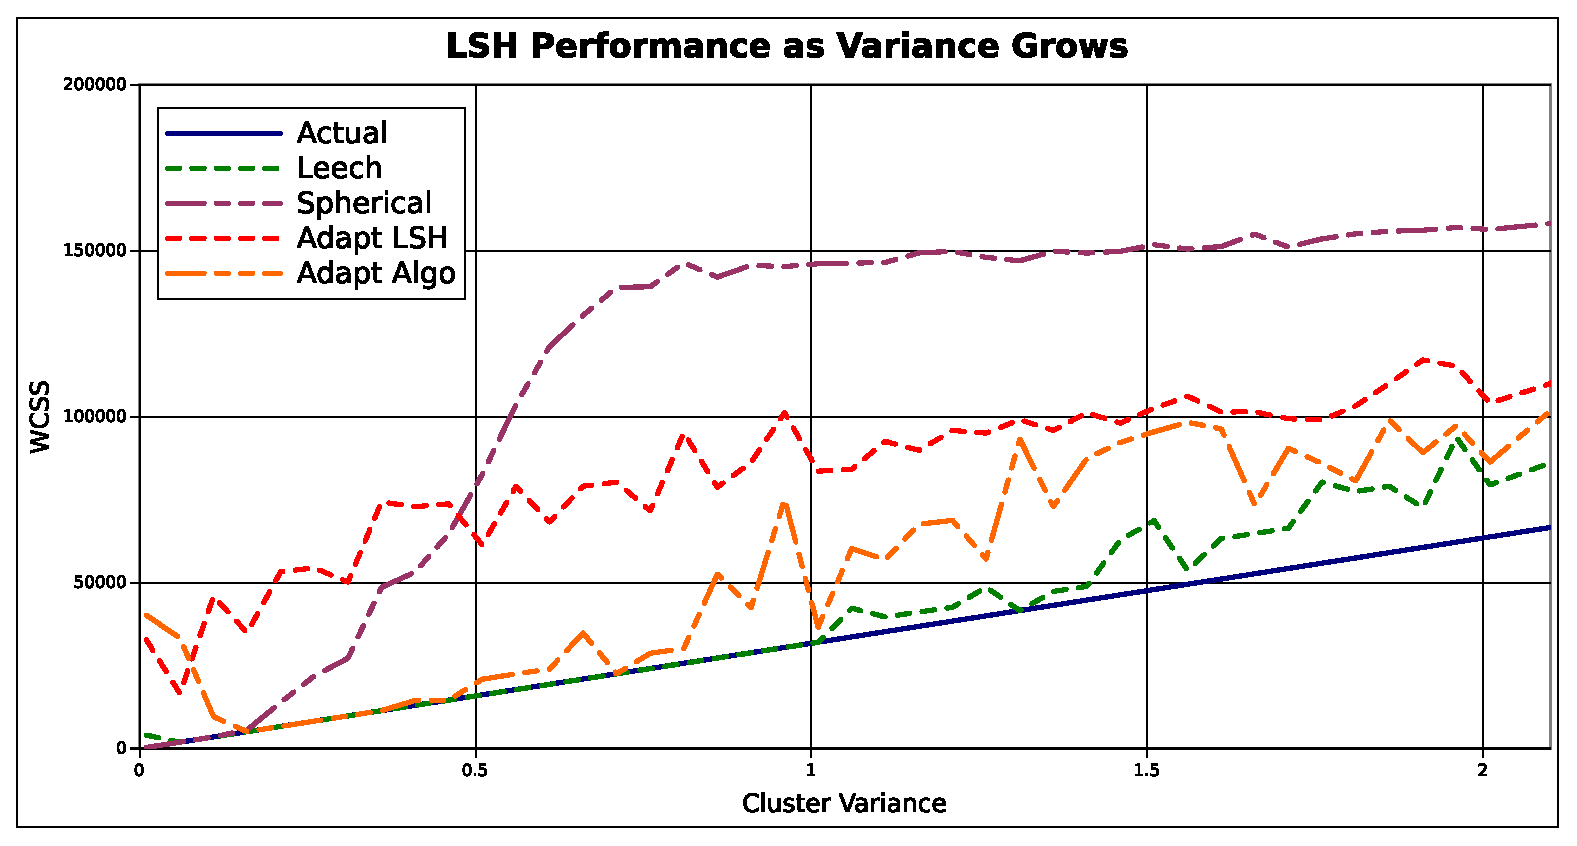
\includegraphics[width=.7\linewidth]{figs/clustervarianceVsDecoders} 
      \caption{Decoders Comparison on Varying Cluster Variance\label{twrpvothers}}
\end{figure}

\section{Streaming RPHash}

In this section, we evaluate the performance of \textsf{streamingRPHash} and compare it against
several other stream clustering algorithms, namely: Streaming $k$-means \cite{braverman}
implementation from S-Space \cite{sspace}, Damped Sliding Window \cite{zhu}, DStream \cite{dstream}
and Biased Reservoir Sampling \cite{ccaggarwal} (described in Section \ref{streamingalgos}).

\textsf{streamingRPHash} uses the optimal configuration described in Section \ref{optimalconf}.  We
apply the stream clustering algorithms on both real-world and synthetic data streams and evaluate
their clustering results based on various external, internal and entropy based clustering validation
measures.  Runtime and memory usage of all algorithms are also captured on a computer having Intel
Xeon X5675 CPU with 6 cores @ 3.07GHz supporting 12 hardware threads.  The operating system is
Debian `stretch' (x86\_64), running on 28 GB memory.  In addition, we assess the impact of noise on
stream clustering algorithms by injecting noise points in synthetic data streams.  Finally, we
perform a preliminary comparison of parallelization of \textsf{streamingRPHash} against streaming
$k$-means.  The results are described in the following subsections.

\subsection{Real-World Datasets}

\begin{figure*}
  \centerline{\includegraphics[width=.9\textwidth]{figs/har_all_measures}}
  \caption{Clustering Smartphone Sensor Data Comparison}{Clustering Results from Smartphone Sensor Data (abbreviations:
    RPH $\rightarrow$ \textsf{streamingRPHash},
    K-M $\rightarrow$ Streaming $k$-means,
    S-W $\rightarrow$ Damped Sliding Window,
    DSt $\rightarrow$ DStream,
    R-S $\rightarrow$ Biased Reservoir Sampling, and
    Base $\rightarrow$ Base Value}\label{human-measures}
\end{figure*}

\begin{figure*}
  \centerline{\includegraphics[width=.9\textwidth]{figs/ujii_all_measures}}
  \caption{Clustering Results from WiFi Location Data}{Clustering Results from WiFi Location Data (abbreviations:
    RPH $\rightarrow$ \textsf{streamingRPHash},
    K-M $\rightarrow$ Streaming $k$-means,
    S-W $\rightarrow$ Damped Sliding Window,
    DSt $\rightarrow$ DStream,
    R-S $\rightarrow$ Biased Reservoir Sampling, and
    Base $\rightarrow$ Base Value}\label{indoor-measures}
\end{figure*}

The algorithms are set up to report clustering results in batches of 500 points.  Performance
results for the \emph{HAR} dataset are shown in Figure \ref{human-measures}.  The plots are
organized into two side-by-side graphs.  The left graph shows the computed values at each 500 points
interval and the right graph is a box and whisker plot that shows the median and quartiles of all of
the sample points for each algorithm.  The results show that \textsf{streamingRPHash} performs on
par with the other algorithms.  The runtime performance is better than most and on par with
streaming $k$-means.  The memory usage is slightly worse than streaming $k$-means, but both are
significantly better (less than half) than the other algorithms studied.

The second dataset is the \emph{UJIIndoorLoc Data Set}\cite{UJII}.  Results from this dataset
are shown in Figure \ref{indoor-measures}.  The plots have the same format as with the previous
study.  Again, the clustering accuracy of \textsf{streamingRPHash} is on par with the other
algorithms while streaming $k$-means is the fastest and has a considerably smaller memory footprint.

\subsection{Scalability Study}

We study the dimensional scalability of stream clustering algorithms by evaluating their clustering
results as the dimensionality of data streams increases.  The purpose of this study is to assess and
compare the accuracy, runtime, and memory usage of \textsf{streamingRPHash} to those of other stream
clustering algorithms with increasing dimensionality.  Labeled data streams of 20,000 points and 10
randomly placed clusters with random multivariate Gaussian distributions are generated using the R
generator (as described in Section \ref{synth_data}).

The dimensionality of data streams, which increases in a sequence from 100 to 5767, follows two
polynomial sequences of the form $d_n = 1.5d_{n-1}$.  The first sequence starts from $d_0 = 100$ and
the second one from $d_0 = 125$.  We do not inject noise points or outliers in these data streams as
we inspect the impact of noise in the next section.  The clustering validation measures are computed
in batches of 1000 points and are plotted against dimensions of data streams.  For ease and clarity
of viewing the WCSSE plot, its values are scaled by diving by the number of dimensions.

Figures \ref{scalability-measures} and \ref{scalability-perf} show the performance results from this
scalability study.  The colored lines in each of these plots represent the mean value and shaded
regions around the lines represent the variance of a measure over all the batches of data points.
The shaded regions on the plots for DStream are wide and clearly visible as its measures have
significantly higher variances than those of other algorithms. In regard to clustering performance, \textsf{streamingRPHash}
performs optimally on all metrics with only one slight variation at 633 dimensions.  This performance
is on par with the other window and sampling streaming clustering algorithms, and outperforms
both DStream and streaming $k$-means.  The Runtime and memory requirements show a different story 
for Reservoir Sampling and Sliding window. Both of these algorithms require significantly more
processing time and space, with significantly worse growth complexity.  This plot shows a major strength
of \textsf{streamingRPHash}, in that it achieves near optimal clustering in linear processing time similar
to streaming $k$-means.

\begin{figure*}
  \centerline{\includegraphics[width=1.1\textwidth]{figs/measure_scale}}
 \caption{Scaling Comparisons External and Internal Measures}{External and Internal Measures from Scaling the Number of Attributes (abbreviations: 
    RPH $\rightarrow$ \textsf{streamingRPHash},
    K-M $\rightarrow$ Streaming $k$-means,
    S-W $\rightarrow$ Damped Sliding Window,
    DSt $\rightarrow$ DStream,
    R-S $\rightarrow$ Biased Reservoir Sampling, and
    Base $\rightarrow$ Base Value}\label{scalability-measures}
\end{figure*}

\begin{figure*}
  \centerline{\includegraphics[width=.9\textwidth]{figs/runtimeGraphs}}
  \caption{Runtime and Memory usage from Scaling}{Runtime and Memory usage from Scaling the Number of Attributes (abbreviations:
    RPH $\rightarrow$ \textsf{streamingRPHash},
    K-M $\rightarrow$ Streaming $k$-means,
    S-W $\rightarrow$ Damped Sliding Window,
    DSt $\rightarrow$ DStream,
    R-S $\rightarrow$ Biased Reservoir Sampling, and
    Base $\rightarrow$ Base Value}\label{scalability-perf}
\end{figure*}

\subsection{Impact of Noise}\label{noise}

\begin{figure*}
  \centerline{\includegraphics[width=1.1\textwidth]{figs/d759_noise}}
  \caption{Injecting Noise into the Data Source.}\label{noise-measures}
\end{figure*}

In this subsection, we assess the clustering results of \textsf{streamingRPHash} in the presence of
random noise in data streams.  We compare the clustering accuracy of \textsf{streamingRPHash} to
those of four other stream clustering algorithms while gradually increasing the percentage of noise
in a data stream.  We arbitrarily choose a dimension = 759 from those used for the scalability study
and generate several data streams with increasing amount of noise.  The percentage of random noise
is increased in an arbitrary sequence.  All of these noisy data streams are generated using the R
stream generator, where each data stream has 20,000 points and 10 randomly placed clusters with
random multivariate Gaussian distributions.  Noise points are assigned labels according to their
nearest cluster centroids.  We use the same clustering validation measures, same batch size (1000
points) and similar plots as with the scalability study.  The results are shown in Figure
\ref{noise-measures}.  The only difference here is that the horizontal axes represent percentage of
noise in data streams. In these figures we see that \textsf{streamingRPHash} performs optimally
in regard to the other algorithms and even baseline for WCSSE and Silhouette, as noise is injected. 
It performs mediocre in the two external metrics ARI and cluster Purity, besting streaming $k$-means 
and DStream.

\section{Tree-Walk RPHash Performance}

In this section we explore the clustering performance of the Tree-Walk RPHash variant (\textsf{TWRP}).  The
\textsf{TWRP} variant of \textsf{RPHash} is what we would consider our best of breed \textsf{RPHash} algorithm.  \textsf{TWRP} uses
information about the data distribution to build adaptive LSH functions, and also more thoroughly
explores the relationships between clusters and encapsulated clusters.  We first compare \textsf{TWRP} to
various other clustering algorithms on real world data, then we explore the scalability, and noise
robustness of \textsf{TWRP}.

\subsection{Real World Data} 
	
The largest and most stable dataset that we've explored so far is the \emph{Human Activity Recognition} dataset \cite{har} dataset.  
The attributes of this dataset are available in Table
\ref{realworld}.  We compare \textsf{TWRP} to standard \textsf{RPHash} as well as our usual set of standard clustering
algorithms, consisting various Agglomerative methods, standard $k$-means, and SOTA.  The results can
be found in Table \ref{perftimetable}.  We captured the runtime (in Secs) performance for all of the
algorithms and results were obtained on a computer with an Intel Core(TM) i7-4770 CPU with 4 cores @
3.40 GHz and 32 GB memory.  Among the compared algorithms \textsf{TWRP} improves upon the performance of standard
\textsf{RPHash} and performs on par with $k$-means and Ward's linkage agglomerative clustering.  The main
benefit however is in its timing results. \textsf{TWRP} is 100x faster than $k$-means, and 2000x faster
than Ward's linkage agglomerative clustering.

\begin{center}
 \begin{table*}
  \centering
\begin{tabular}{|c|c|c|c|c|}\hline
\cellcolor[gray]{0.9}\textbf{Algorithm}	&\cellcolor[gray]{0.9}\textbf{ARI}	&\cellcolor[gray]{0.9}\textbf{Purity} &\cellcolor[gray]{0.9}\textbf{WCSSE} &\cellcolor[gray]{0.9}\textbf{Time} \\ \hline
\cellcolor[gray]{0.9}\textbf{Kmeans}		&0.461  &0.6   &182168.7&24.746\\\hline
\cellcolor[gray]{0.9}\textbf{Single Link}  		&0      &0.189 &556519.1&413.88\\\hline
\cellcolor[gray]{0.9}\textbf{Complete Link}  		&0.327  &0.377 &222044.4&414.33\\\hline
\cellcolor[gray]{0.9}\textbf{Average Link}  		&0.332  &0.359 &236142.8&414.1\\\hline
\cellcolor[gray]{0.9}\textbf{Ward's}		&0.491  &0.66  &191441.1&414.45\\\hline
\cellcolor[gray]{0.9}\textbf{SOTA}  		&0.314  &0.397 &210490.1&14.244\\\hline
\cellcolor[gray]{0.9}\textbf{RPHash}		&0.363  &0.508 &210628.6&0.4838\\\hline
\cellcolor[gray]{0.9}\textbf{TWRP}	&0.449	&0.609 &194688.7&0.2617\\\hline
\end{tabular}
\caption{Clustering Performance and Timing}\label{perftimetable}
\end{table*}
\end{center} 

\subsubsection{Synthetic Data}

In this experiment we generated datasets with successive dimensionality in $\mathbb{R}^{100}$ to
$\mathbb{R}^{7000}$ space.  Each dataset consists of 10000 vectors equi-probable chosen from a set of
10 univariate Gaussian clusters.  Figures \ref{perfdim1},\ref{perfdim2},\ref{perfdim3} give the
clustering performance of \textsf{TWRP} compared to other clustering algorithms for the metrics, ARI , Purity
and WCSSE on the generated datasets.  \textsf{TWRP} performs optimally for all dimensions, equaling the agglomerative
methods.  It is also stable, compared to standard \textsf{RPHash} and $k$-means.


\begin{figure*}
    \centering
    \includegraphics[width=1\linewidth]{figs/ari_synthetic_2} 
    \caption{ARI Synthetic} \label{perfdim1}
\end{figure*}
\begin{figure*}
    \centering
    \includegraphics[width=1\linewidth]{figs/purity_synthetic_2} 
    \caption{Purity Synthetic} \label{perfdim2}
\end{figure*}
\begin{figure*}
    \centering
    \includegraphics[width=1\linewidth]{figs/wcsse_synthetic_2} 
    \caption{WCSSE Synthetic}\label{perfdim3} 
\end{figure*}

\subsubsection{Noise Stability}

An important test of a clustering algorithm's versatility is its robustness to noise.  In general,
real world data will contain at least some level of noise due to systematic errors in measurement.
In this experiment we will generate datasets with varying amount of noise. We chose a dimensionality
of 1000 dimension and inject noise varying from 5 percent to 50 percent of the overall dataset size
in increments of 5 percent.  The noise vectors generated were assigned the label of the closest
cluster center.  The results of the noise injection tests are plotted in Figures
\ref{noiseacc1},\ref{noiseacc2},\ref{noiseacc3}, with ARI, Purity, and WCSSE being tracked
respectively.

\begin{figure*}
    \centering
    \includegraphics[width=1\linewidth]{figs/ari_noise_2} 
    \caption{ARI Noise}\label{noiseacc1} 
\end{figure*}
\begin{figure*}
    \centering
    \includegraphics[width=1\linewidth]{figs/purity_noise_2} 
    \caption{Purity Noise}\label{noiseacc2} 
\end{figure*}
\begin{figure*}
    \centering
    \includegraphics[width=1\linewidth]{figs/wcsse_noise_2} 
    \caption{WCSSE Noise}\label{noiseacc3} 
\end{figure*}

We observe that until the noise percentage reaches 40 the accuracy of both the \textsf{RPhash} algorithms
are far better than the other six standard algorithms. Thereafter as the noise grows beyond 50
percent and the signal to noise ratio is very low, all the algorithms tend to perform poorly.

\subsubsection{Scalability}

Table \ref{scalability} summarizes the timing results on synthetic datasets.  The data sets were
generated using the R data generator discussed in Section \ref{synth_data} to generate 10000 vectors from $k=10$
univariate clusters, with varying dimensionality.  Results for all clustering algorithm timings were
obtained on a computer with Intel(R) Xeon(R) E5-2670 @ 2.6 GHz with 16 cores and 64 GB RAM.  While
Table \ref{scalability} gives a detailed measure of the scalability for all comparison clustering
algorithms, Figure \ref{twrp_scale} shows difference between the \textsf{RPHash} algorithms and only the two
faster comparison clustering methods.  This is due to the agglomerative methods being so much slower
that they would skew the output plot making it useless for comparison.  In this experiment we see again
that the scalability of the \textsf{RPHash} algorithms far exceeds the other compared methods.  While SOTA and $k$-means
achieve, what appears to be linear complexity growth, the \textsf{RPHash} methods, appear constant in comparison.  This 
of course is not true and they share a similar linear complexity with  SOTA and $k$-means. We 
can verify this in the scalability Table \ref{scalability}, but should note that the difference in processing time, 
between \textsf{RPHash} algorithms, SOTA, and $k$-means is significant.

\begin{center}
 \begin{table*}
 \centering
\begin{tabular}{|c|c|c|c|l|l|}\hline
\cellcolor[gray]{0.9}\textbf{Dimension}&\cellcolor[gray]{0.9}\textbf{KMeans}&\cellcolor[gray]{0.9}\textbf{AverageLinkage}&\cellcolor[gray]{0.9}\textbf{SOTA}&\cellcolor[gray]{0.9}\textbf{RPHash}&\cellcolor[gray]{0.9}\textbf{TWRP}\\

\cellcolor[gray]{0.9}&\cellcolor[gray]{0.9}&\cellcolor[gray]{0.9}\textbf{Link}&\cellcolor[gray]{0.9}
\cellcolor[gray]{0.9}&\cellcolor[gray]{0.9}\textbf{Leech}&\cellcolor[gray]{0.9}\\\hline 

\cellcolor[gray]{0.9}\textbf{100}&3.9656&47.46&13.758&0.4890&0.1638\\\hline
\cellcolor[gray]{0.9}\textbf{300}&13.3796&194.121&23.797&0.4782&0.1638\\\hline
\cellcolor[gray]{0.9}\textbf{500}&32.92&454.777&36.046&0.5594&0.3005\\\hline
\cellcolor[gray]{0.9}\textbf{700}&77.7298&672.759&48.963&0.6174&0.3642\\\hline
\cellcolor[gray]{0.9}\textbf{900}&117.3675&929.6&61.759&0.7052&0.4078\\\hline
\cellcolor[gray]{0.9}\textbf{1000}&142.2341&1064.178&68.86&0.7206&0.4318\\\hline
\cellcolor[gray]{0.9}\textbf{1500}&237.0007&1789.142&96.795&0.8233&0.5392\\\hline
\cellcolor[gray]{0.9}\textbf{2000}&366.0743&2450.813&127.972&0.8796&0.6548\\\hline
\cellcolor[gray]{0.9}\textbf{2500}&431.5876&3108.654&155.968&0.9997&0.8050\\\hline
\cellcolor[gray]{0.9}\textbf{3000}&542.0223&3771.886&185.23&1.1122&0.8917\\\hline
\cellcolor[gray]{0.9}\textbf{3500}&631.8423&4435.349&220.562&1.2421&1.0229\\\hline
\cellcolor[gray]{0.9}\textbf{4000}&741.915&5080.802&248.669&1.3157&1.1498\\\hline
\cellcolor[gray]{0.9}\textbf{4500}&811.3911&5725.061&274.983&1.3986&1.2873\\\hline
\cellcolor[gray]{0.9}\textbf{5000}&909.223&6362.574&301.314&1.5095&1.4128\\\hline
\cellcolor[gray]{0.9}\textbf{5500}&975.2703&7006.91&324.314&1.5977&1.5392\\\hline
\cellcolor[gray]{0.9}\textbf{6000}&1076.882&7645.155&359.911&1.6805&1.6157\\\hline
\cellcolor[gray]{0.9}\textbf{6500}&1187.6062&8278.964&400.767&1.7933&1.7266\\\hline
\end{tabular}
\caption{Scalability Study.}\label{scalability}
\end{table*}
\end{center}

\begin{figure*}
    \centering
    \includegraphics[width=.8\linewidth]{figs/Scalability_Synthetic} 
    \caption{SCALABILITY Synthetic}\label{twrp_scale}
\end{figure*}

\subsection{Tree Walk RPHash (\textsf{TWRP}) Results on Word2Vec Data}

In this section we used the GoogleNews \cite{googlenews} Word2Vec dataset to compare the clustering
and timing performance of \textsf{TWRP} with $k$-means++.  Word2Vec data is particularly interesting, because
it often contains very large, high dimensional, and dense, data vectors that often occupy lower
dimensional embeddings.  However, due to the size of the observations, it is unlikely that a ground
truth will be available.  Observation can verify certain subjective aspects of the data clustering,
such as two similar words or concepts being labeled in the same cluster, but an overall labeling is
usually unavailable.  For this experiment, we rely on the WCSSE only to act as a performance metric.
We could theoretically compute other external metrics, such as Silhouette and Dunn Index however
given the size of the GoogleNews data set, it is computationally infeasible.  In addition, we do not
have a defined number of clusters.  Figure \ref{w2vwcss} gives the WCSSE for a sequence of possible
values of $k$ for \textsf{TWRP} and $k$-means++.  Likewise, Figure \ref{w2vratio} gives the ratio of the
$k$-means++ WCSSE and \textsf{TWRP} WCSSE.  Under the assumption that $k$-means++ finds nearly the optimal
WCSSE, we can regard \textsf{TWRP} as an $\epsilon$-error equivalent.  As \textsf{TWRP} appears to be outperformed in
regard to WCSSE, by $k$-means++, it is important to focus on some of its advantages, namely its
speed.  Figure \ref{w2vproctime} gives a comparison of the two algorithms in regard to processing
time.  As, is clear in other runtime performance tests, the TWRP algorithm scales linearly with the
data size, and overall requires far less computation than $k$-means, and similar algorithms.

\begin{figure}[t]
        \centering
        \includegraphics[width=.75\textwidth]{figs/w2vratio_wcss.pdf}
	\caption{WCSSE KMeans++ to \textsf{TWRP} Ratio}\label{w2vratio}
\end{figure}
\begin{figure}[t] 
        \centering
        \includegraphics[width=.85\textwidth]{figs/w2vwcss.pdf}
	\caption{WCSSE Comparison Results}\label{w2vwcss}
\end{figure}
\begin{figure}[t]
        \centering
	\includegraphics[width=.85\linewidth]{figs/w2vtime.pdf}
	\caption{Processing Time Comparison}\label{w2vproctime}
\end{figure}


\section{RPHash Parallelism}

\textsf{RPHash} was designed with the intent of being naively parallelizable.  As with many parallel
adaptations of well-known machine learning algorithms, the influence of Amdahl's Law appears during
parallelization efforts due to unavoidable sequential bottlenecks as the number of processing nodes
increases.

In this section we compare the three proposed variants of \textsf{RPHash} in regard to parallel speedup.  Our
testing was done on an 8-core Intel Xeon CPU with 4 threads per core, for a total of 32 sequential
threads.  The parallelism was implemented similar to our target platforms of map-reduce and spark
streaming interface.

\subsubsection{Standard RPHash}

The standard \textsf{RPHash} algorithm parallel implementation consists of an equal partitioning of vectors
to processing units.  In the map phase, each processing unit applied the per vector process to their
respective subset of vectors in parallel.  The threads then performed a log reduction sum of the
counts of hash collisions in the thread's respective subset of vectors. The result of the first
phase is a set of the densest hash bucket, IDs.  The second phase then proceeds byt redistributing
the data vectors to processing nodes, and accumulating a centroid for vectors that produce hashes
that collide with the dense set of hash bucket IDs. These centroids are then reduced through a
weighted sum log reduction of the centroids.

\subsubsection{TWRP}

The tree walk variant consists of a similar equal partitioning of vectors among processing nodes as
the standard \textsf{RPHash} variant.  Similarly, each node accumulates a separate MinCount data
structure.  Once all vectors have been processed, the MinCount structures are merged, for all
indices.  The result is the complete MinCount structure, from which the tree based, off-line step of
\textsf{TWRP} proceeds sequentially. In our tests, we only tested the sequential off-line step, however,
various parallel depth first search methods could be employed to improve performance and parallel
speedup.

\subsubsection{Streaming RPHash}

The \textsf{streamingRPHash} variant is discussed last because it differs the most from the previous
algorithms.  Namely, the \textsf{streamingRPHash} algorithm has a different data access structure.
\textsf{streamingRPHash} receives vectors one after another, and updates a Count-Min sketch.  To parallelize
the streaming version we process the projections and hashing of vectors in parallel, but must use a
thread safe priority queue, for updating frequent centroids.  While thread safety tends to inject
sequential bottlenecks in otherwise parallel code, the bottleneck is often reduced, by the low
probability of colliding hashes for frequent and infrequent vectors.  For highly clusterable data
the ratio of frequent and infrequent vectors is low.  While for real world vectors with a high
degree of noise, the ratio is much higher, resulting in better parallelism.

\subsection{Parallel Speedup Results}

Figure \ref{minskispeedup} shows the parallel speedup as a function of processing cores for the 3
\textsf{RPHash} variant algorithms proposed.  The data source consists $n= 10^7$ vectors in
$\mathbb{R}^{1000}$ uniformly distributed among 10 Gaussian distributed clusters, and 1 uniformly
distributed 'noise' cluster.  The experiment consisted of generating the vectors and storing them in
main memory, then iteratively increasing the number of processing units for each of the three
described \textsf{RPHash} algorithms.  The results of these tests show that the standard \textsf{RPHash} has the
greatest potential for distributed scalability, followed by \textsf{TWRP}, then \textsf{streamingRPHash}.
All of the speedup curves show characteristic diminishing returns of Amdahl's Law curves.

\begin{figure}
  \centerline{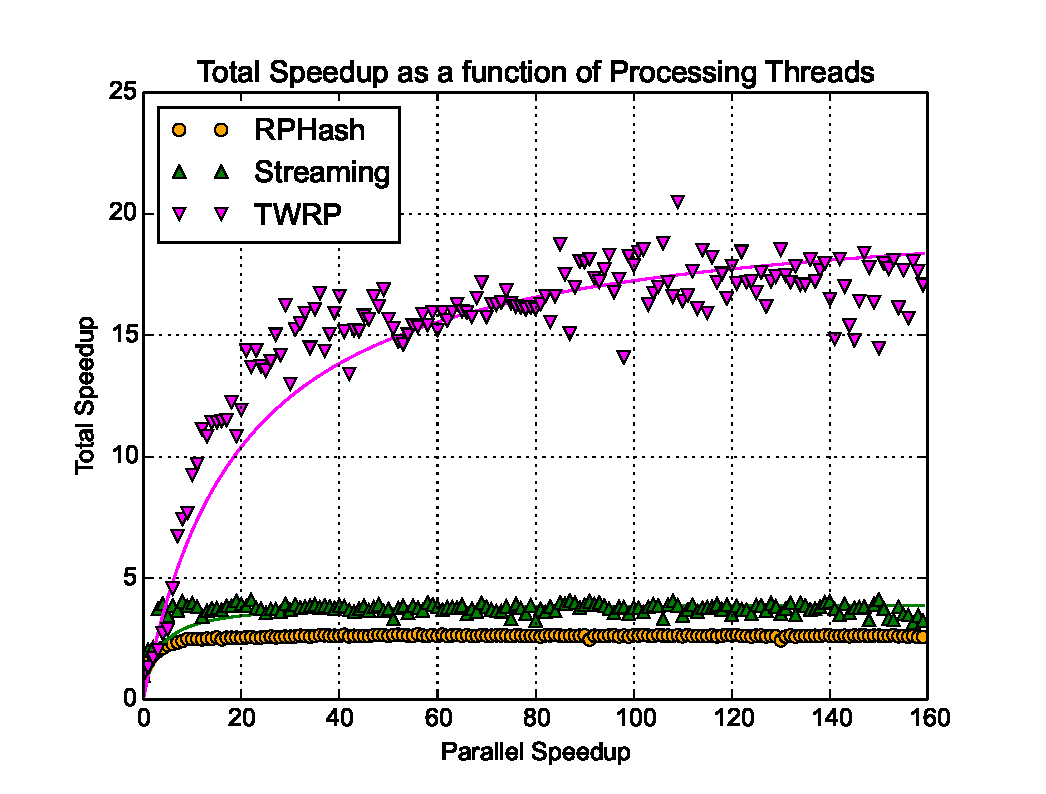
\includegraphics[width=.8\textwidth]{figs/minskispeedup}}
  \caption{Speedup Comparison between RPHash Algorithms}\label{minskispeedup}
\end{figure}

\section{Security Performance}

Due to the inability to anticipate all possible cryptographic attacks on de-anonimization, a
qualitative measure of data obfuscation is developed for comparing a fully qualified vector $v\in
\mathbb{V}^d$ with its corresponding projected vectors $v'\in \mathbb{V}^d$.  This metric referred to
as $k$-anonymity allows us to evaluate the probability of de-anonymization of a vector.

$v'$ is the inverse projection of $u\in \mathbb{V}^s$ that results from the random projection of
$v$.  Destructive data obfuscation occurs if the distance between $v'$ and $v$ is greater than the
distance between $v$ and some other vector $\hat{v}\in \mathbb{V}^d$.  The inverse projection matrix
$R_{d\rightarrow s}^{-1}$ will be used to map $u$ back to $v$'s original subspace.  The two
equations below describe the projection of $v$ to $u$ and the theoretical inverse of the projection
from $u$ to $v'$ under the matrix transform $R_{d\rightarrow s}$ where $d>s$.

$$ u = \sqrt{{\frac{n}{k}}}R_{d\rightarrow s}^Tv $$
$$ v' = \sqrt{{\frac{k}{n}}}u^T R_{d\rightarrow s}^{-1} $$

The above inversion is theoretical however due to the orthogonal projection $R_{d\rightarrow s}$
being non-square and not invertible.  Therefore, for a projection matrix $R_{d\rightarrow s}$ the
least squares solution $\hat{R}_{d\rightarrow s}^{-1}$ will serves as the optimal inverse of the
projection.  Even in the not strictly orthogonal random projection case (as in Achlioptas
\cite{Achlioptas01} and \textsf{RPHash}) the least-squares solution will result in an over-determined
system of equations.  Which implies that any pseudo-inverse projection of a vector in $V^s$ to $V^d$
will result in unrecoverable data loss for non-trivial cases (\emph{i.e.},
$<$\textbf{0}$>$,$<$\textbf{1}$>$).  The goal in testing the security of \textsf{RPHash} is to show
that the data loss is sufficient to make it impossible for an attacker to re-associate the projected
vectors.  A formal definition of the requirement for destructive data obfuscation follows:

$$
s(v,v') = ||v,v'||_{2} 
$$

$$
\forall\{v,v'\} \in V , \exists {\hat{v}} \in V : s(v,v')>s(\hat{v},v) \text{ where }
\hat{v}\neq v ~ \textrm{or} 
$$

$$
Pr(NN((v\cdot R)\cdot \hat{R}^{-1},V)=v)\lesssim {1\over{||V||}}
$$

Due to the often sensitive nature of medical data, we give a real world example based on the MIMIC
II \cite{MIMICII} data set.  Figure \ref{projrecov} shows the $k$-anonymity curve for vector
recoverability demonstrating the effectiveness of random projection for providing vector
anonimization.  The overall bi-clustering in full and reduced dimensions showed little to no
degradation over full and reduced subspaces down to 10 dimensions.  This is further corroborated on
additional data in Bingham \cite{bingham}.  Following the above definition of destructive data
obfuscation, we constructed a test on the MIMIC II data.  The Moore-Penrose inverse generated from
the reciprocal of the singular value decomposition diagonal matrix is generated from the projection
matrix and used as the least squares inverse projection to remap the projected vectors to their
original subspace.  The nearest neighbor method was then used to query the original set of vectors
to see if a vector can be re-associated with itself.  In the results it is clear that as
dimensionality increases, the probability of re-association converges to random coincidence of a
Bernoulli trial $((1-(1/n))^n) \approx .363$.  The successful re-associate rate follows an inverse
power-law like distribution.

\begin{figure}
\centering
 \includegraphics[width=.7\textwidth]{figs/recovery}
  \caption{Probability of Vector Re-association for MIMIC II BioMetric Signatures}\label{projrecov}
\end{figure}

In regard to security performance, it is fairly clear that data becomes unrecoverable when the
difference between the original data embedding and the projected space exceeds 75 dimensions.  Given
that \textsf{RPHash}'s native clustering space is 24 dimensions, this case occurs for a wide variety of high
dimensional datasets, namely those that exceed 99 dimensions.

\chapter[Theory]{Algorithmic Complexity and Theory}\label{theory}
In this section we analyze the performance of the proposed variants of \textsf{RPHash} in regard to their asymptotic complexity.
Although adversarialy crafted datasets can be NP-Hard for iterative update methods like Hartigan and Wong's $k$-Means
algorithm \cite{Vattani}, they often fair much better in practice. In common practice $k$-Means tends to be described 
as having $\Theta(n\log\log(n))$-complexity, or sometimes simply $\Theta(n)$. While this fact is useful in terms of
scalability, the effects of constant factors can vary widely in practice in regard to processing time. For this
reason we prefer the results presented in Chapter \ref{experiments} for exact timing results. None-the-less we provide
a complexity analysis for \textsf{RPHash}, and in all cases find them to be linear, and predictable.

\section{RPHash Complexity}
In the experimental section we empirically show that \textsf{RPHash} has linear complexity. However in this section
we take a more theoretical approach to proving this claim. Namely we show that \textsf{RPHash} has asymptotic complexity,
that is linear to the input size. 

\subsection{Algorithmic Complexity}
The simplest form of \textsf{RPHash}, the two pass approach. This approach has a rather simple complexity derivation.  The
algorithm passes once over all vectors, performing a projection and a hash.  The dimensionality of
the projections $m$ depends on the number of input vectors $n$ and not on the dimension of the
vectors $d$.  From JL-Lemma, we set this dependence as $m=\Theta(\log(n))$, where the problem input
space is $N=nd$.  Projection requires $\Theta(\log(N/d)N/3)$ steps, with generally small constant
factors using the db-friendly projection of \cite{Achlioptas01}.  When $\log(N/d)$ is near $c^3$,$c$
is constant and projection is linear.  Hashing on the projected vectors is performed
in constant time for certain lattices (\emph{e.g.,} $\Lambda_{24}, E_8$), or using $m=\log(d)$, 
$\Theta(2\log(d))$-time.  Updating the counters in the first phase is performed in constant time,
through a hash-table, or count sketch.  Thus, the overall complexity of phase one is
$\Theta(\log(N/d)N/3 + C ) = \Theta{N}$.

The second pass of 2-pass \textsf{RPHash} consists of the same process as the first pass to project and look
up vectors and their respective hash ids.  However in the second phase we also compute the centroids
for dense hash buckets.  The worse case complexity of the update process is $\Theta(nd)$ or
$\Theta(N)$ assuming all vectors are contained in a dense cluster.  The overall complexity of the
second pass is $\Theta(N+N) = \Theta(N)$.  Examining both phases, we have an overall complexity of
$\Theta(\log(N/d)N/3 + C ) + \Theta(N) + \Theta(N) = \Theta(N)$ which when $\log(N/d)\approx 3$, is
effectively linear.

\section{Streaming RPHash Complexity}
In this section we discuss the compute and memory complexities of the streaming variant of \textsf{RPHash}
(\textsf{streamingRPHash}.  One of the principal goals for a streaming algorithm, and basic
requirements, is that the computational complexity is at least sub polynomial and the Storage
complexity is sub-linear. We prove both of these claims in the following two sections.

\subsection{Computation Complexity}
One of the earliest streaming solutions for the approximate \emph{$k$-HH} algorithms is the
Count-Min sketch data structure \cite{cormode2}.
Count-Min sketch can be used to solve the approximate \emph{$k$-HH} problem with only the addition
of a priority queue using $\Theta({1\over \epsilon} \log {1 \over \delta})$ space with error
$(1-\epsilon)f$, where $f$ is the minimum frequency $m \over k$ to be considered frequent.  The
complexity of \textsf{streamingRPHash} is:
$$\Theta \bigg( NP\bigg(  {{Md}\over{3}} +\log(d)\big(\log(k)+d+2d^2\big)\bigg ) \bigg)$$
when using $P$ database friendly projections from $M$ to $d$, SLSH decoding complexity ($2d^2$), a
balanced priority tree (with $\Theta(\log(k))$ insertion and constant time removal), and a blurring
factor $\log(d)$.  The projection step ${{Md}\over{3}}$ tends to dominate when $M>>d$.  If we remove
the constant factor, constant number of projection $P$ and subspace $d$, we have complexity of
$\Theta(NM)$ , leaving only the input and thus, the algorithm is linear in $n$.
 
\subsection{Storage Complexity}
Streaming algorithms are potentially unbounded in size. While the limit is finite, it does 
impose an additional storage requirement on our algorithm. In particular, our algorithm must
grow sub-linear, otherwise the stream is no different than reading a large data set into memory.

Using the Count-Min sketch to store the approximate hash counts gives us a bound on storage
complexity that is a product of the stream size and desired error rate.  
Cormode \cite{cormode2} shows that the storage complexity of the Count-Min Sketch with error tolerance
$\epsilon$, where $\epsilon = 1-\delta$ is $\Theta( B ln({{1}\over{\delta}}))$, where $B$ is the number of
independent objects that need to be counted.
If then use a bounded $k$HH-Tree of size $klog(k)$ to maintain the $klog(k)$ densest
vector centroids, we come to a total space requirement of 
$$\Theta((d k log(k))ln({{1}\over{\delta}}))$$
If we assume $k\approx \log\log(n)$. We get a final complexity of
$$\Theta(d \log\log(n/d) \log\log\log(n/d)) =\Theta(d\log\log(n)) $$
 
\section{TWRP Complexity}
The complexity of \textsf{TWRP} is similar to that of \textsf{streamingRPHash}.  More precisely, consider its
complexity from the perspective of a per vector complexity, with an on-line and off-line step.  For
each vector \textsf{TWRP}  must compute the projection, and update the sketch.  Projection using the db
friendly approach of Achlioptas \cite{Achlioptas01} can be performed in $\Theta(dm/3)$ operations
where $d$ is the original dimensionality, $m$ is the projection sub-dimension and
$m=\Theta(\log(n))$ where $n$ is the total number of input vectors.  Assuming $n$ is large, but not
infinite, the projection step is $\Theta(d\log(C))$, where $C$ is a constant related to $log(n)$ by the JL 
lemma.  From the complexity analysis of Count-Min Sketch for \textsf{streamingRPHash}, we have an additional 
complexity factor of $\Theta(ln({{1}\over{\delta}}))$.  Following this, the time to update all levels of the hash are
consequently the tree depth and dimensionality of the projected subspace.  Leading to an overall per
object complexity of $\Theta( d m^2 ln({{n}\over{\delta}}) )$.  The Count-Min Sketch update factor
is effectively constant for a reasonable chosen $\delta=.01$.  Furthermore, following
Johnson-Lindenstrauss's bound on sub-dimension representations, reasonably $m =
\Theta({{\log(d)}\over {\epsilon}}) $, resulting in a complexity of $\Theta(
m d\log(C)\log(C))=\Theta(m d \log^2(C))$ .

The off-line step consists of the min-cut tree exploration.  The exploration follows a depth first
search tree-traversal for candidate clusters, which has a worse case complexity when exploring all
non-leaf nodes of $\Theta( 2^{d-1})$.

\subsection{Storage Complexity}\label{twrperror}
The count-min tree is generally never explored in its entirety. Instead only nodes corresponding to
dense hash regions are traversed.  Furthermore if we store the counts approximately in the Count-Min 
sketch, the storage requirement can be further reduced.  Therefore
if we only traverse dense clusters, using a Count-Min Sketch, we get the standard $k$-Heavy-Hitter formulation.
This formulation has storage complexity $\Theta( ln({n\over \delta}))$ for n items, and a desired error 
$\delta = 1-\varepsilon$.  
Although the Count-Min Sketch size is parametric in the desired error bound, for 
acceptable error rates, we must store a sketch of centroids that is at least $\Theta( m ln({n\over \delta}))$.
This will violate the streaming data requirement when $\delta > n \mathbb{e}^{-n/m}$.
However, we can use the tree structure to our advantage, to correct errors after the fact.

\subsubsection{Count-Min Tree Error}

Interestingly, this leads to a boost in the general Count-Min Sketch error, because we can
recover errors using adjacent parent and sibling nodes in the induced space cut tree. In other words, 
by exploring neighboring tree nodes, we can confirm or refute the approximate count of a node. This
is particularly useful for the possible occurrence of a short LSH ID, colliding with a much longer
ID. Which would result in a false branch. To illustrate this, we can consider the case where we
have two sibling nodes, with approximate cardinality, 5 and 100. The parent node cardinality should
be near or exactly 105, otherwise we can suspect a collision error in the larger node. Using 
the triangle inequality, we can confirm or refute the approximate counts within this hierarchy of nodes.
Furthermore, if the parent and sibling counts do not fully satisfy the triangle inequality requirement,
we can query the counts of their parent and child nodes to find additional support, and correct approximate 
count errors.

For count min-sketch alone, we choose the number of sketches to be $ln({n\over \delta})$\cite{cormode2}. 
However using tree count adjacency we can reduce the count error to $\sqrt{\delta}$ and set the number of sketches
$\Theta({e \over \varepsilon})$. Resulting in a total storage requirement of 
$\Theta(m{e \over \varepsilon}ln({{nlog(d)}\over{(\sqrt{\delta)}}}))$.
 
\section[RP Speedup]{DB Friendly Random Projection Speed Up}

From \cite{Achlioptas01} we know that a set of vectors can be projected into a lower dimensional
embedding $\Re^d$ where $d \propto {\Omega({{ \log(n) }\over {\epsilon^2 \log 1/\epsilon} })}$ with
low $\epsilon$-distortion if projected using a matrix formed as:

$$r_{ij}= \sqrt{3}
\begin{cases}
+1,  \text{with probability } {1 \over 6}\\
0,  \text{with probability } {2 \over 3}\\
-1,  \text{with probability } {1 \over 6}\\
\end{cases}
$$
where: \\
$n$ - number of vectors\\
       $m$ - vector dimensionality\\
       $k$ - projected space dimensionality\\

\noindent
The above result allows us to avoid the computationally expensive task of matrix orthogonalization.
This point is due to the high probability of randomly generated vectors being nearly orthogonal as $n$
increases.  Furthermore, the above result suggests we can avoid the costly generation of the normal
variate, as the above suffices to give a nearly normal distribution about the point in the projected
subspace.  Computing and multiplying still naively requires $nmk$ operations.  Below we will show
how to get this down to $\log({3\over2})nmk$ operations.  A trick, since multiplying by \(0\) is has
no effect on the row vector sums, is to select $n\over 3$ of the indices from a given vector, and
multiplies them by $+1/-1$ evenly (thus our $1\over6$ probability).  Random selection however
requires us to either store collisions and re-select indices until they do not collide.  The odds of
a perfect non-colliding intersection are tremendously low due to the birthday problem (yields
$\approx {{2} \over{3 n}} $).  So we need to account for intersections.  The amount of intersection
however is bounded.  To assess this bound we use Riemann Sums and Union Bound Estimate simultaneously
to obtain the integral:

$${\int ^{n\over3}_0 {1\over{n-x} }dx}= ln({3\over2}),$$


\noindent
For the selections $$\underset{x\to\infty}{lim}({1\over n}+{1\over {n-2}}...+{1\over{n-n/3}})$$
By changing our range from 0 to \(1\over3\), to $ln({3\over2})$, we now generate our selections and
compensate for the intersections.  The evenness of $+1/-1$ assures that even though we are
generating more indices, the generated distribution will still be symmetric about 0.  Although we can
similarly calculate the probability of the additional selections colliding with the selected
${2\over3} - ln({3\over2})$, the recursion converges quickly and the effects are negligible.  An experiment
was performed for a set of uniform random vectors $x\in X $ where $d=5000$. In the experiment we compared shuffling 
a full list and selecting the first $n/3$ indices, to our proposed selection of $n\ln({3\over2})$ from the full 
range of indices one after another. In this experiment we get the following deviation between $p_1$- db-friendly 
projection and $p_2$ - sequential random selection projection.
$$\|p_1^{\intercal}X - p_2^{\intercal}X\|=.00001$$. 

\chapter{Conclusions}\label{conclusions}

All variants of \textsf{RPHash} share a number of similar performance advantages over other traditional
methods while also suffering similar drawbacks.  Subsequent attempts to mitigate these drawbacks
resulted in the various version of \textsf{RPHash} and configurations.  In this section we discuss those
common attributes as well as a breakdown of the variant specific attributes and how they compare to
other clustering algorithms.

\section{Clustering Performance}

In this section we discuss how \textsf{RPHash} clustering performance compares to classic and state-of-the art
clustering algorithms.  While the primary goal of clustering is ill-posed, performing well on an
ensemble of clustering metrics is generally regarded as an overall useful measure of clustering
performance.

\subsection{RPHash}

Table \ref{compareOtherAlgo} gives an exhaustive comparison of the standard \textsf{RPHash} algorithm to
various other common clustering methods.  In this section we focus only on the listed clustering
performance.  Regarding clustering performance, we report measures for \emph{adjusted rand index}
and \emph{cluster purity}.  \textsf{RPHash}'s performance is highly dependent upon the dataset being
clustered.  In general it performs better than most of the agglomerative methods for all datasets.
The exception for agglomerative methods is the Ward's Linkage, which performs better in some of the
chosen datasets.  This performance often echoes that of $k$-means performance, on the same
datasets.  While $k$-means tends to outperform \textsf{RPHash} in regard to overall performance, none of the
performances are better by a significantly large margin.  SOTA seems to perform most similarly to
\textsf{RPHash}, with similar ARI and Purities for all datasets.  The overall goal however is not that \textsf{RPHash}
outperforms other metrics in terms of clustering performance, rather that it is comparable, with the
an advantage in processing speed.  We investigate this further in Section \ref{rptiming}.

Table \ref{localWinners} gives more detailed performance for an optimized configuration of \textsf{RPHash}
against $k$-Means.  As before, \textsf{RPHash} and $k$-Means alternate between best performance, with only
minor deviations between the two.  The reconfigurability of \textsf{RPHash} is important in this case because
it can be optimized for the particular dataset, while $k$-means is less flexible in configuration.

\subsection{Streaming RPHash}

The performance of \textsf{streamingRPHash} is shown in Figure \ref{indoor-measures} and
Figure \ref{human-measures} as a function of streamed batches of data.  On both datasets
\textsf{streamingRPHash} tends to find a good local minima for the Within-Cluster Sum of Squared
Error metrics.  However, \textsf{streamingRPHash} tends to suffer on some external metrics such as
the adjusted rand index, and internal metrics that tend to favor cluster separability, such as Dunn
Index and Silhouette Index.  Further analysis of these results show a bias in
\textsf{streamingRPHash} that suggests it favors solutions to the facility location problem over the
more general clustering problem.  This may be exacerbated by the fact that \textsf{streamingRPHash}
does not specifically label noise or outlier vectors, which can result in poorer values pertaining
to Silhouette Index and Dunn Index.  This is mainly due to noise clusters skewing the inter/intra
-cluster distance ratio.

The performance of \textsf{streamingRPHash} on synthetic datasets with varying dimensions is shown in
Figure \ref{scalability-measures}.  For synthetic datasets \textsf{streamingRPHash} does quite well,
matching the optimal performance of the best stream clustering algorithms. In all cases it
outperforms Streaming $k$-Means and Damped Sliding Window.

The scalability of \textsf{streamingRPHash} for Runtime and memory is shown in Figure
\ref{scalability-perf}.  As expected the resource requirements of \textsf{streamingRPHash} and
streaming $k$-means are substantially lower than those of other tested algorithms.  This advantage
becomes increasingly significant as the dimensionality of the input vectors grows.  Although
streaming $k$-means maintains a consistently better bound on both memory and processing time, the
overall growth complexity is similar, which suggests optimizations to \textsf{streamingRPHash} could
put it in reach or streaming $k$-means' performance.

The noise study demonstrates an addition benefit of \textsf{streamingRPHash}.  As expected, a
gradual decrease in clustering accuracy of all algorithms is observed as the amount of noise
increases in the data stream.  However, there are some interesting patterns in clustering results
produced by \textsf{streamingRPHash}.  Its clustering accuracy clearly exceeds that of other
algorithms in the presence of 2\% noise.  As the amount of noise begins to increase in the data
stream, Damped Sliding Window and Biased Reservoir Sampling seem to produce better clustering in
terms of external measures.  However, even with the increasing noise, \textsf{streamingRPHash}
continues to give the best clustering results in terms of internal measures.  In particular, its
WCSSE values remain the lowest, and sometimes lower than baseline values, even in the presence of
noise as high as 60\% and 75\%.  This can be explained if we look into how labels are assigned to
random noise points at the time of data stream generation.  As mentioned before, each noise point is
assigned to a cluster whose centroid is the closest to that noise point.  Thus, a noise point, which
is assigned to a cluster $i$, may actually be closer to the boundary of another cluster $j$.
Therefore, it is possible that a clustering algorithm places a noise point in a \emph{more
  appropriate} cluster than the data stream generator does.  In other words, the clustering
algorithm may be able to find better centroids to incorporate noise points, thus producing more
compact clusters than ground-truth partitions.  In this case, the clustering algorithm will produce
better values of internal measures than the baseline values.  On the other hand, since external
measures try to capture the agreement between ground-truth partitions and clusters detected by an
algorithm, the values of external measures will clearly remain low.  This is why
\textsf{streamingRPHash}, when applied on noisy data streams, performs much better in terms of
internal measures.  The apparent decrease in values of external measures is merely due to the
disagreement with ground-truth labels of noise points.

To summarize our findings from the scalability study: we discover a major strength of
\textsf{streamingRPHash} and conclude that the algorithm is capable of producing perfect clustering
when the data stream consists of a mixture of Gaussian distributions without any noise.  For real
world, and data containing a significant amount of noise, it may be useful to augment
\textsf{streamingRPHash} with the ability to label observations as noise.

\subsection{Tree Walk RPHash}

On real world and synthetic datasets, the Tree-walk RPHash algorithm tends to perform better than
the standard \textsf{RPHash} and \textsf{streamingRPHash} algorithms.  In contrast the Adaptive LSH algorithm
in both the Streaming and Standard \textsf{RPHash} algorithm has a slightly mixed result.

In Figure \ref{twrpvothers} we see that standard \textsf{RPHash} and the Leech decoder outperforms the
adaptive LSH algorithm and the \textsf{TWRP} algorithm.  While this result is in opposition of our claim that
the \textsf{TWRP} is best among \textsf{RPHash} variants, it is important to note that the experiment was performed on
a highly synthetic dataset with no noise, and tightly clusterable data.  The test in fact is very
similar to the results in Figure \ref{bbvar} where the Leech Lattice decoder was well suited to
finding tight, uniform clusters scaled between -1 and 1.  It is not until we look at more
realistically generated datasets and robust clustering metrics that we see the advantage of \textsf{TWRP}.
Figures \ref{perfdim1}, \ref{perfdim2}, and \ref{perfdim3} show \textsf{TWRP} performing optimally for all
datasets at all dimensions, while the standard \textsf{RPHash} algorithm and $k$-Means show considerable
variance in Purity, ARI, and WCSSE.  In Figure \ref{w2vwcss} and Figure \ref{w2vratio} we look at the raw
WCSSE scores, and the ratio of WCSSE for \textsf{TWRP} and the $k$-Means++ algorithm on 1000 dimensional,
real world, Word2Vec data.  Overall, \textsf{TWRP} performs within $5.1\%$ of $k$-Means++.  This is significant
if we consider the scalability difference between \textsf{TWRP} and $k$-Means++.  Figure \ref{w2vproctime}
shows these differences, and while $k$-Means++ seems to grow quadratically with the number of
clusters, \textsf{TWRP} remains constant.  This is significant, because \textsf{TWRP} could potentially output any
number of micro-clusters to some, more robust machine learning algorithm, with no change in
processing time requirement.

\section{Noise Resilience}

All variants of the \textsf{RPHash} algorithms are noise robust.  This is primarily due to the density mode
search common in all algorithms, ignoring data that resides outside the partition region.  In Figure
\ref{noise-measures} we show the performance of \textsf{streamingRPHash} in regard to injected noise.  In
regard to WCSSE, \textsf{streamingRPHash}s outperforms all other clustering algorithms on noise resilience.  While among
other performance metrics, it tends to be in the top three.  Standard \textsf{RPHash} and \textsf{TWRP} are compared
in Figures \ref{noiseacc2}, \ref{noiseacc2} and \ref{noiseacc2} on ARI, Purity and WCSSE as a function of
injected noise.  For ARI and Purity, \textsf{TWRP} outperforms standard \textsf{RPHash} and the other comparison
algorithms up until the highest levels of injected noise $>35\%$.  Standard \textsf{RPHash} outperforms \textsf{TWRP}
on WCSSE metrics, but not by a very large margin.

\section{Timing Results}

A principal focus and motivation for this work, is to reduce the time and overall complexity of
current clustering methods.  As expected, \textsf{RPHash} and its variants outperform all other tested
clustering methods on processing speed and asymptotic complexity.  Time results at linear with
smaller constant factors than many other clustering methods.

\subsection{RPHash}\label{rptiming}

In Table \ref{compareOtherAlgo} we see that the standard \textsf{RPHash} algorithm often bests comparable
clustering algorithms by at times orders of magnitude on larger datasets.  Furthermore the growing
deviation between processing times in regard to dataset sizes suggests and overall asymptotic
complexity difference over other tested algorithms, which is verified in the previous sections
runtime analysis.  While agglomerative methods and SOTA tend to require considerably more time to
process than \textsf{RPHash}, $k$-Means is sometimes regarded as a near linear runtime algorithm
($\theta(loglog(n)*n)$).  However in a direct comparison shown in Table \ref{localWinners} we can
see that \textsf{RPHash} outperforms $k$-Means considerably on runtime.  This suggests that while $k$-Means may
have near linear asymptotic complexity, it exhibits considerable constant factor offsets.

\subsection{Streaming RPHash}

Similar to standard \textsf{RPHash}, \textsf{streamingRPHash} performs well on runtime.  While standard
\textsf{RPHash} was not compared against streaming $k$-Means, \textsf{streamingRPHash} was.  Streaming $k$-Means
in Figure \ref{indoor-measures} and Figure \ref{human-measures} outperforms \textsf{streamingRPHash} on
runtime.  However both algorithms exhibit similar scalability, as suggest by Figure
\ref{scalability-perf}.  It is likely that these performance differences could be overcome with
minor implementation optimization.

\subsection{TWRP}

The scalability with respect to dimension of \textsf{TWRP} and standard \textsf{RPHash} is shown in Figure
\ref{twrp_scale}.  In the plot we see that there is no contest between the \textsf{RPHash} algorithms and the
comparison algorithms SOTA and $k$-Means.  While the Table \ref{scalability} shows an even more
dramatic difference between both versions of \textsf{RPHash} and the agglomerative algorithms.  \textsf{TWRP} is
almost 688 and 4795 times faster than $k$-means and agglomerative hierarchical respectively for the
noise datasets having dimensions 10000x6500. We can see the growth of time as the dimension
increases in Figure \ref{twrp_scale} . RPhash and \textsf{TWRP} has almost no growth when compared to the
other algorithms.

Figure \ref{w2vproctime}, Table \ref{scalability} and Table \ref{perftimetable} provide similar evidence
regarding the superiority or \textsf{RPHash} algorithms in general
With the complexity growth of \textsf{RPHash} being nearly linear, with small constant factor offsets.
Therefore we can see that one of the biggest advantages of \textsf{RPHash} is that it achieves such
comparable clustering accuracy with minimal costs of runtime . This makes \textsf{RPHash} suitable for
applications where the dimension or volume of data is very high.

\section{Parallelism}

A primary focus of the \textsf{RPHash} algorithms is to enable naive parallelism through the coordination of
generative mathematical functions and approximate data sketches, instead of costly verbose
interprocess communication.  The results in Figure \ref{minskispeedup} show that our assumptions about
\textsf{RPHash} parallelism, are to some degree, correct.  For data centric algorithms like \textsf{RPHash}, the ratio
of parallel to sequential code, per Amdahl's law, is strongly dictated by the input data size.
However to not bias our parallelism with the input IO of our test machine's memory subsystem, all
parallel experiments were done on in memory datasets, resulting in a limit to the overall amount of
achievable parallelism.  It is our belief that larger datasets may show further advantages for
\textsf{RPHash} in regard to parallel speedup.

Standard \textsf{RPHash} appears to enjoy the greatest advantage in regard to parallel speedup. The results
for \textsf{RPHash} were edited to remove, outlier data points in which memory contention for many nodes,
caused errors as parallelism grew.  This is more an artifact of our chosen method of parallelism,
than that of an intrinsic algorithm design.  Namely, standard \textsf{RPHash} tends to use significantly more
memory per core than our sketch based algorithms.  This Memory requirement presented itself when
scaling to more processing nodes, and caused a memory bottleneck around 15 nodes.  Fifteen nodes
however is a reasonable baseline to establish the predictable parallelism.  For the intended
distributed implementation of \textsf{RPHash} in MapReduce or Spark, it is unlikely these physical memory
restrictions would exist.

Interestingly, \textsf{TWRP} which would presumable be sequentially bound by the off-line Tree walk procedure
and per vector, shared sketch update step, actually parallelizes quite well.  The likely reason for
this is that the off-line step does not contribute significantly to the overall number of
computations required for both on-line and off-line processing steps.  Furthermore, the shared memory
environment of our experimental setup, allows for fast access to the Count-Min Cut Tree structure.
In the distributed setting, this would not be the case.  However, due to the additive nature of the
Count-Min Sketch, completely independent update of the Count-Min sketch would be trivial and would
only require a $\theta(log(N))$ number of steps to reduce the $N$ sketches.

\textsf{streamingRPHash} suffered a poorer than expected speedup performance.
\textsf{streamingRPHash} utilized vector parallelism, in which processing nodes were scheduled by a
master node, to the first available thread.  This naturally results in a sequential bottleneck at
the master node.  However, it additionally stresses cache prediction, in real world CPUs, due to our
greedy vector-to-CPU assignment.  The greedy assignments are strongly influenced by the chosen LSH
algorithm, which in this experiment was the Leech Decoder, which is determined by the randomly
generated data vectors.  This cache pressure along with the sequential bottleneck, make
\textsf{streamingRPHash} a poor candidate for shared memory system parallelization.  However, for
distributed systems in which vectors are fetched from a remote source, the parallelism should only
be bound by the intermittent off-line steps.  In contrast, both \textsf{TWRP} and standard \textsf{RPHash} were able to
partition the problem equally among processing nodes and then work on the sets of vectors
independently.

An alternate hypothesis however, is that our results may be somewhat under represented due to our
test system only having 16 physical cores and 32 threads due to Hyper-Threading, instead of 32
truly independent processing nodes.  Hyper-Threading is a technology that effectively shares the
resources of a single processing pipeline, between two processing workloads, with the assumption
that underutilized processing sub-units will achieve better overall utilization.  This however is not
completely equivalent to two independent processing units.  The saturation of one unit, such as the
Floating Point sub processing unit, could cause a bottleneck.  Furthermore, hyper-threading is also
bound by there only being one physical, memory management unit per core, which could be a source of
further IO saturation.  Another likely candidate for our sub-linear speedup performance could be our
test system's Quick Path Memory controller, resulting in non-uniform memory data access patterns.
Attempts were made to optimize this access pattern through both the Java NUMA flag, and the
operating system `numactl' meta-processing environment.  Both alterations failed to achieve
significantly different results (timing was worse on all tests).  These possibilities further
suggest that a completely independent distributed processing environment may achieve better overall
parallelism.

\section{Overall Conclusion}

The \textsf{RPHash} algorithms combines approximate and randomized methods in a new way to solve
issues of scalability and data security for cluster analysis on distributed data.  The runtime and
clustering performance of our \textsf{RPHash} algorithms are similar to that of the standard $k$-means
clustering algorithm, with the added benefit of being scalable to very large datasets.  This
randomized, clustering algorithm is well suited for ill-posed, combinatorially restrictive problems
such as clustering and partitioning.  This assertion is complemented by a similar inversion
regarding clustering and computing, in which real world problems tend to converge much faster than
adversarially crafted worse-case problems.

The principle assumption in this work is that approximate and exact clustering, are qualitatively
similar due to noise, redundancy, data loss, and the curse of dimensionality.  Furthermore, the
addition of random noise to the clustering dataset resulting from the random subspace projection
requirement, provides some degree of non-deterministic process, so subsequent iterations of the
algorithm could potentially find better results.  Making the process of finding better clustering
results, a matter of available processing time and resources.  Furthermore, the destructive
projection process affords us a certain degree of data privacy while requiring no additional
processing.

\subsection{RPHash Conclusions}

The \textsf{RPHash} algorithm offers a fast highly scalable algorithm for data clustering that shows
potential for distributed computing that can benefit well from addition processing resources, and is
secure.  \textsf{RPHash}'s simple straightforward structure results in a predictable time requirement.  The
processing time predictability is beneficial for time dependent cases where completion time is more
important than minor errors in clustering accuracy.  Overall, \textsf{RPHash} is much faster than other
clustering algorithms.  Some drawbacks of the standard \textsf{RPHash} algorithm, is that the results can be
order dependent, and sometimes unstable.  Multiple runs can fix some of these issues, but the
overall stability may be an outstanding problem, that we suggest \textsf{TWRP} remedies.

\subsection{Streaming RPHash Conclusion}

\textsf{streamingRPHash} Is a fast accurate single pass clustering method for high dimensional data
streams.  The growing number of massive, high dimensional streaming data sources can take advantage
of the benefits of quick, accurate, scalable and distributed processing of \textsf{streamingRPHash}.
We show that our method is faster than most of our comparative streaming clustering algorithms. 
while performance is underwhelming on the HAR dataset, \textsf{streamingRPHash} does quite well on
the UJII dataset.  The deviation in performance between datasets suggests that
\textsf{streamingRPHash} may not be well suited for all datasets.  However, when data is well
behaved, containing predominantly spherical clusters in high dimensional space,
\textsf{streamingRPHash} outperforms all other streaming clustering methods.  This may be a result
of the sub-space projection, being well equipped to capture the overall data variance for these types
of datasets.  Another feature of \textsf{streamingRPHash} is that it is robust to noise,
outperforming all other clustering algorithms on clustering metrics.  These benefits however are
overshadowed by \textsf{streamingRPHash} processing efficiency, scalability and memory usage.
\textsf{streamingRPHash} compares well to Streaming $k$-means in timing and memory usage.  While
shared memory parallelism is below our expectations, the potential for distributed processing, is
positive, and would likely exceed the scalability of streaming $k$-means which incurs a sequential
bottleneck when checking and updating a shared list of nearest cluster centroids.

\subsection{TWRP Conclusions}

In this work we introduced the Tree-Walk Random Projection (\textsf{TWRP}) clustering technique for
clustering large datasets with log-linear processing complexity.  We applied our clustering
technique on real and synthetic data of varying noise levels.  Our method performed comparable to
various other common clustering methods, while improving significantly upon the overall required
processing time.  \textsf{TWRP} improves upon standard \textsf{RPHash} clustering performance and in many cases
performs better than $k$-means and similarly to Ward's Linkage hierarchical agglomerative
clustering.  Importantly, it does so, while achieving a similar processing time requirement and
scalability as standard \textsf{RPHash}.  Furthermore the \textsf{TWRP} algorithm improves upon \textsf{RPHash}'s already
relatively good noise suppression performance.  \textsf{TWRP} also improves upon \textsf{RPHash} by offering more
stable results between runs, that border on deterministic behavior.  Another advantage of \textsf{TWRP} is
that is shows strong potential for shared memory and distributed parallelism.  In addition, \textsf{TWRP} is
also amenable to streaming environments, due to its base structure being the Count-Min Cut-Tree.
The Count-Min Cut-Tree is an error bounded constant memory sketch, that succinctly encodes the
required data structure of the off-line clustering process.

\subsection{Code Repository}
The \textsf{RPHash} Java source code is released under an open source license and is freely
available at \url{github.com/wilseypa/rphash-java}.  Python versions of \textsf{TWRP} are available on-line at
\url{https://github.com/leecarraher/PyRecRPHash}.  Plots and figures are available by request
\url{mailto://leecarraher@gmail.com}

\section{Future Research}\label{further}
In this section we give suggestions for potential future research following the \textsf{RPHash} clustering framework.  We discuss
a further distributed framework for \textsf{streamingRPHash}, and \textsf{RPHash} as a pre-clustering technique for more robust
clustering methods like topological data analysis(TDA).
We also suggest more practical implementation improvements like GPU processing. Lastly we discuss the potential of the 
general Count-Min Cut Tree as a general space partitioning sketch.

\section{Spark Implementation}

\begin{figure}
    \centerline{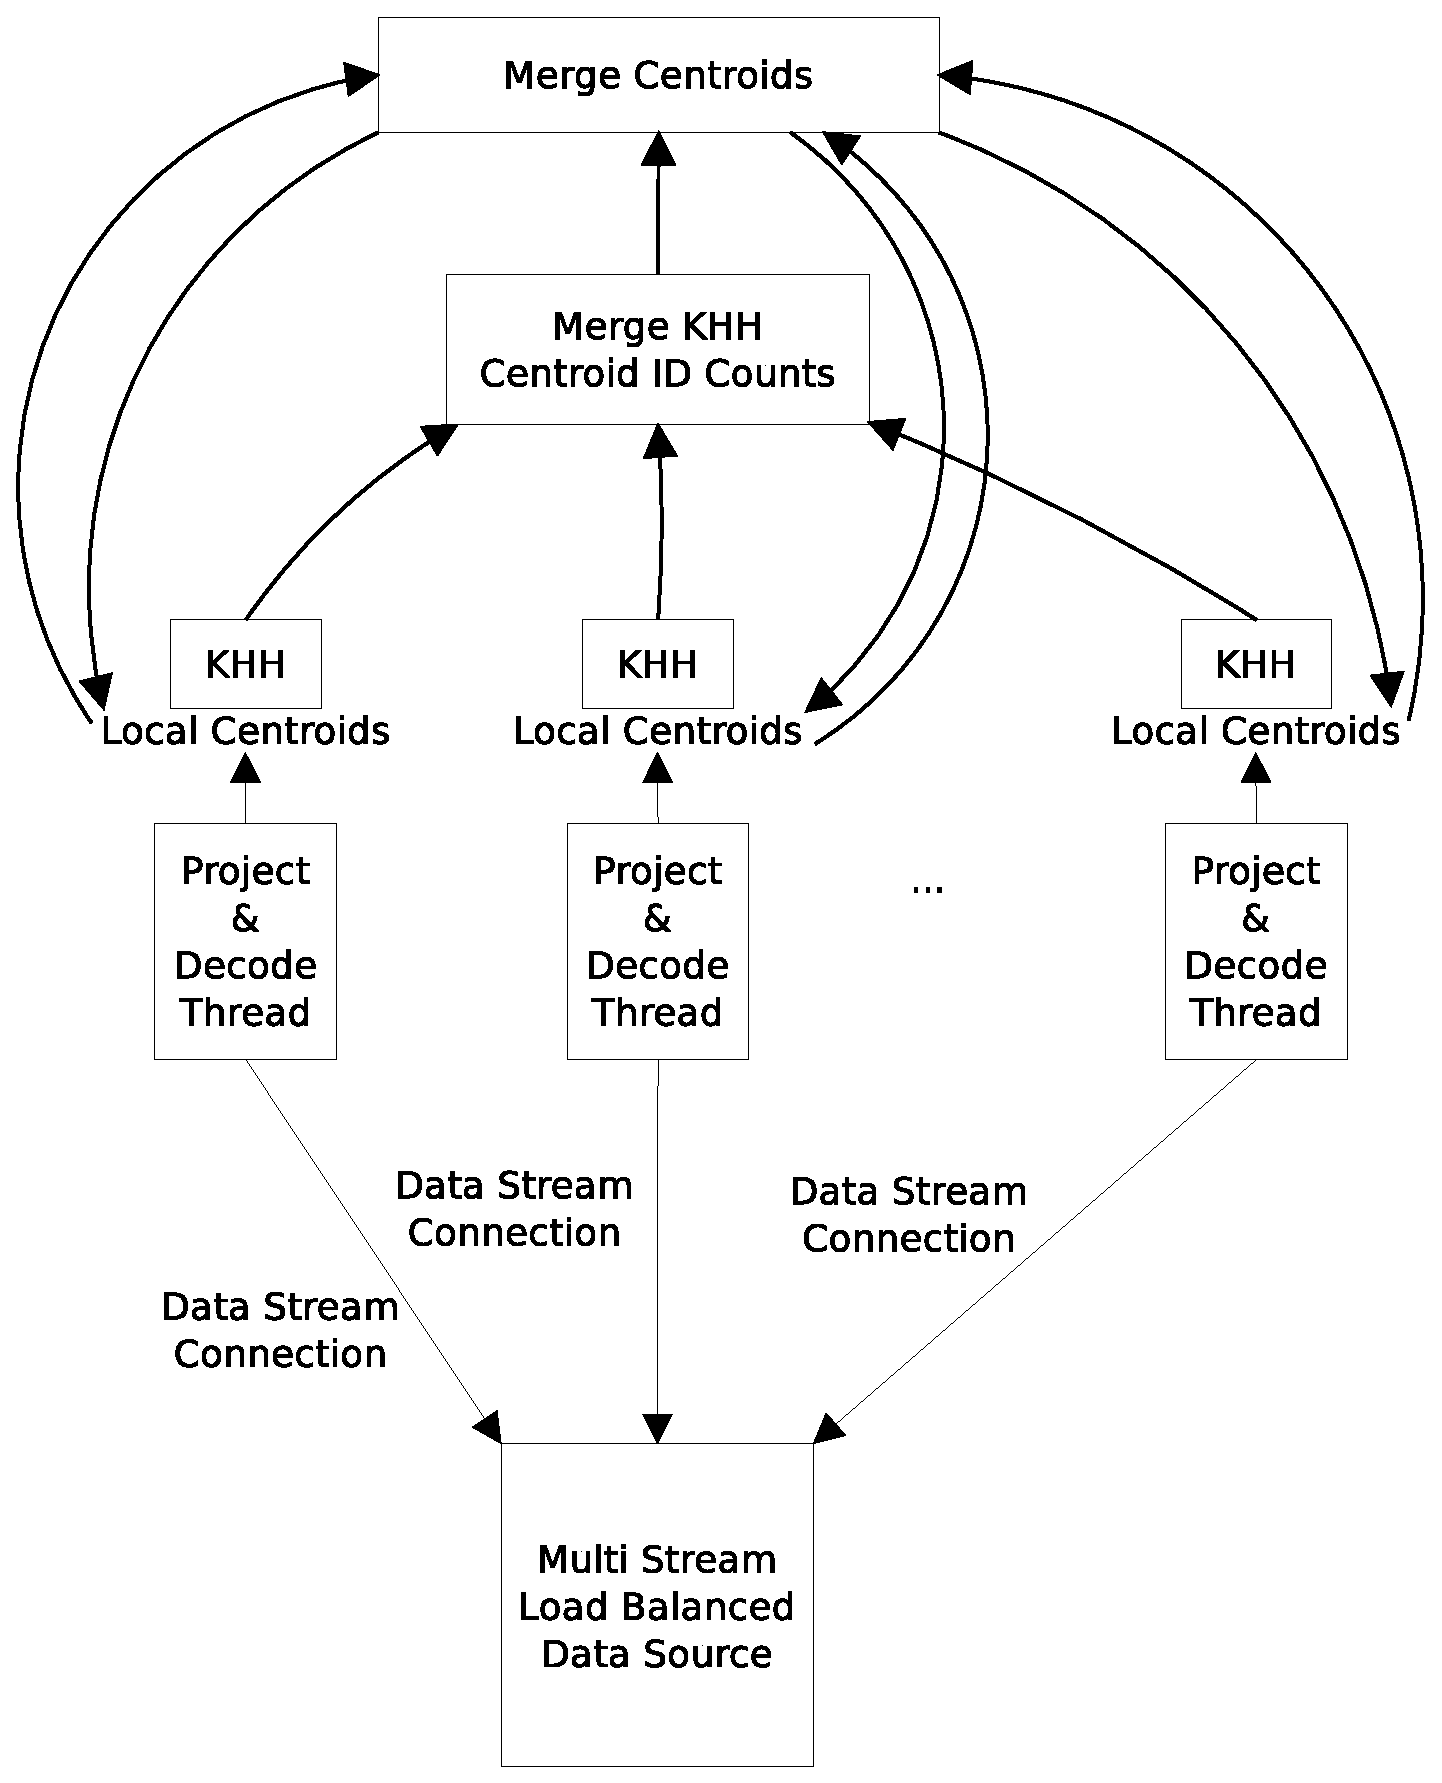
\includegraphics[width=.7\textwidth]{figs/sparkrp}}
    \caption{Spark Streaming RPHash Diagram}\label{sparkrp}
\end{figure}

Spark is a distributed computing framework loosely based on functional parallelism that runs on
Hadoop and other similar frameworks.  Spark is similar in design to MapReduce functional dissection
for parallel algorithms, however, unlike the standard Hadoop MapReduce algorithm, it is geared toward
multi-pass processing common in machine learning algorithms, by leveraging RAM caching of persistent
states between Map and Reduce phases.  Furthermore, Spark allows for streaming interfaces for
parallel processing, capable of extending the \textsf{streamingRPHash} algorithm.  A future direction
for \textsf{streamingRPHash} would be to utilize the input stream methods in spark, to implement 
\textsf{streamingRPHash} as a fully distributed stream based clustering method.  The implementation could read
streams independently from disconnected data streams, building independent data structures, and merging the 
results when requested.  Similar to the \textsf{streamingRPHash} diagram given in Figure \ref{rphash}, we give a 
distributed extension in Figure \ref{sparkrp}. 

\subsection{Topological Data Analysis}

An interesting emerging field in machine learning is topological data analysis(TDA). TDA attempts to
overcome some of the issues inherent with orthogonal metric data embeddings by regarding not just
the data, but the connectivity between the data.  Somewhat similar to manifold learning methods, in
which data is regarded as being embedded in some complex manifold, TDA goes further, by removing the
restriction that a surface be locally differentiable. In this way, surfaces can have holes, and true
discontinuities.

While TDA work is still emerging, there is a significant gap between theoretical understanding and
practical application.  In particular, many TDA algorithms are graph based and therefore,
combinatorially bound.  However, by using the concept of micro-clusters, arbitrarily available through
\textsf{RPHash} clustering, with no computation penalties, one could potentially reduce the complexity of
TDA algorithms, to these representative micro-clusters, followed by subsequent refinements. 

\section{GPU Leech}

Previous work \cite{carraher} on a graphics processing unit (GPU) implementation of the Leech Decoder for LSH could readily be
used to accelerate the \textsf{RPHash} algorithm.  While performance monitoring showed the principal
occupation of \textsf{RPHash} was in the projection step, accelerating just the LSH may only result in a
small speedup.   However, if we were to combine both the projection and a GPU based implementation of
LSH, we may be able to take advantage of GPU memory locality, and achieve considerably high GPU core
occupancy (a principle measure for GPU parallelism).

\subsection{Bounded Error Compressed Cut Tree}


While the results from Tree Walk Random Projection Hash are promising, a more interesting data
structure is defined that may have application beyond cluster analysis. In particular, this structure,
which will be referred to as a \emph{Bounded Error Compressed Cut Tree} has the potential of 
accelerating and making feasible a variety of interesting learning and data space exploration problems. 

We briefly review its structure here.  In \textsf{TWRP} we partitioned a data set by a sequence of orthogonal
vectors corresponding to the origin of each subsequent dimension.  This partitioning results in a 
$d$ length LSH encoding for every vector.  The hashes are then stored as a compressed representation
in the Count-Min Sketch.  As an aside, while we make the restriction that all hyperplanes intersect the origin,
BECC-Trees could also be composed of any set of hyperplanes rotated any number of times.  This
structure which we treat as a vector density oracle for \textsf{TWRP} clustering could be used similarly, for a variety
of other purposed. The basic setup would involve changing either the tree traversals method, or by storing some 
alternative metric in the nodes.  The tree, again never being fully realized, uses the Count-Min Sketch as an
 approximate partitioning oracle.  Therefore any tree based solution to a graph problem in which a
cut oracle would be helpful, could be solved in $1\over \epsilon$ space.

The true power of this structure comes 
of course comes from the parameterization of the Count-Min Sketch, which allows one to set the level of 
acceptable error, for tree based oracle problem.  The Count-Min Sketch constrained to elements in a tree
can compress any exponentially large space partitioning problem, and is certainly worth further investigation.  
Our Bounded error compressed cut trees certainly demonstrate this property for clustering.  In addition, the ability 
of BECC Trees to consume a potentially unbounded data stream, and store only a sketch of its current structure to 
later be scrutinized and reconstruction is potentially applicable to off-line data stream inquiry.  

%The \textsf{streamingRPHash} algorithm combines approximate and randomized methods in a
%new way to solve issues of scalability and data security for cluster analysis of data
%streams.  The runtime and Precision-Recall performance of \textsf{streamingRPHash} is
%similar to that of the standard KMeans clustering algorithm, with the added benefit of
%being applicable to infinite data streams.  This randomized, clustering algorithm is well
%suited for ill-posed, combinatorially restrictive problems such as clustering and
%partitioning.  This assertion is complemented by a similar inversion regarding clustering
%and computing, in which real world problems tend to converge much faster than
%adversarially crafted worse-case problems.

%The principle assumption in this work is that approximate and exact clustering, are
%qualitatively similar due to noise, redundancy, data loss, and the curse of
%dimensionality.  Furthermore, the addition of random noise to the clustering dataset
%resulting from the random subspace projection requirement, provides some degree of
%non-deterministic process, so subsequent iterations of the algorithm could potentially
%find better results.  Making the process of finding better clustering results, a matter of
%available processing time and resources.

%Clustering has long been the standard method used for the analysis of labeled and
%unlabeled data.  Clusterings effects intrinsically identify dissimilar and similar objects
%in a dataset, often unattainable through standard statistical methods.  Single pass, data
%intensive statistical methods are often the primary workhorses for database processing of
%business logic and other domains, while clustering is often overlooked due to issue in its
%scalability.

%Applications such as Micro Array clustering, Protein-Protein interaction clustering,
%medical resource decision making, medical image processing, and clustering of
%epidemiological events all serve to benefit from larger dataset sizes that
%\textsf{streamingRPHash} enables.


\section*{Acknowledgments}

Support for this work was provided in part by the National Science Foundation under grant
ACI--1440420.



%% if you plan to have appendicies uncomment the next two lines.  the \appendix
%% command will alter the \chapter command to format it as an appendix.  pretty
%% easy. 

%%\appendix
%%\chapter{Appendix A}\label{appendixA}



%% these commands tell latex to put the references here.  for the most part you
%% should just leave this stuff alone.

\bibliographystyle{abbrv} \markright{ }
\bibliography{refs}



\end{document}
